%-----------------------------------------------------------------------------------------------%
%
% Oktober 2022
% Template Latex untuk Laporan Kerja Praktek Program Studi Sistem informasi ini
% Dikembangkan oleh Daffa Takratama Savra (daffatakratama13@gmail.com)

% Template ini dikembangkan dari template yang dibuat oleh Inggih Permana (inggihjava@gmail.com).

% Orang yang cerdas adalah orang yang paling banyak mengingat kematian.
%
%-----------------------------------------------------------------------------------------------%

%-----------------------------------------------------------------------------------------------%
% Dilarang mengedit file ini, karena dapat merubah format penulisan
%-----------------------------------------------------------------------------------------------%

\documentclass[12pt, a4paper, onecolumn, oneside, final]{report}
\usepackage{kontrol/uinsuskakerjapraktek}
%-----------------------------------------------------------------------------------------------%
%
% Oktober 2022
% Template Latex untuk Laporan Kerja Praktek Program Studi Sistem informasi ini
% Dikembangkan oleh Daffa Takratama Savra (daffatakratama13@gmail.com)

% Template ini dikembangkan dari template yang dibuat oleh Inggih Permana (inggihjava@gmail.com).

% Orang yang cerdas adalah orang yang paling banyak mengingat kematian.
%
%-----------------------------------------------------------------------------------------------%

%-----------------------------------------------------------------------------------------------%
% Dilarang mengedit file ini, karena dapat merubah format penulisan
%-----------------------------------------------------------------------------------------------%

\var{\fakultas}{Fakultas Sains dan Teknologi}
\var{\fakultasInggris}{Faculty of Science and Technology}

\var{\programStudi}{Program Studi Sistem Informasi}

\var{\gelar}{Sarjana Komputer}

\var{\universitas}{Universitas Islam Negeri Sultan Syarif Kasim Riau}

\var{\kota}{Pekanbaru}

\var{\alamatUniversitas}{Jl. Soebrantas, No. 155, Pekanbaru}

\var{\rektor}{Prof. Dr. Hairunnas, M.Ag}
\var{\dekan}{Dr. Hartono, M.Pd}
\var{\kaprodi}{Eki Saputra, S.Kom., M.Kom}
\var{\kaprodinip}{NIP. 198307162011011008}
\var{\sekretarisprodi}{Siti Monalisa, S.T., M.Kom}

%-----------------------------------------------------------------------------%
% Judul BAB
%-----------------------------------------------------------------------------%
%

\var{\lembarPengesahanInstansi}{LEMBAR PENGESAHAN INSTANSI}
\Var{\lembarPengesahanProdi}{LEMBAR PENGESAHAN PROGRAM STUDI}
\var{\kataPengantar}{KATA PENGANTAR}
\var{\abstrak}{ABSTRAK}
\var{\babSatu}{PENDAHULUAN}
\var{\babDua}{LANDASAN TEORI}
\var{\babTiga}{TUGAS KERJA PRAKTEK}
\var{\babEmpat}{ANALISA DAN HASIL}
\var{\babLima}{PENUTUP}
%-----------------------------------------------------------------------------------------------%
%
% Oktober 2022
% Template Latex untuk Laporan Kerja Praktek Program Studi Sistem informasi ini
% Dikembangkan oleh Daffa Takratama Savra (daffatakratama13@gmail.com)

% Template ini dikembangkan dari template yang dibuat oleh Inggih Permana (inggihjava@gmail.com).

% Orang yang cerdas adalah orang yang paling banyak mengingat kematian.
%
%-----------------------------------------------------------------------------------------------%

\var{\judul}{IMPLEMENTASI SISTEM INFORMASI INVENTARIS LABORATORIUM MENGGUNAKAN \textit{FRAMEWORK} CODEIGNITER 4}
\var{\penulis}{HAFIZ ARYAN SIREGAR}
\var{\nim}{12150310904}
\var{\tahun}{2023}

\var{\pembimbingpertama}{TENGKU KHAIRIL AHSYAR, S.KOM., M.KOM}
\var{\pembimbingpertamanip}{198505202023211020}

\var{\prefiknomorinduksatu}{NIP}
\var{\namaInstansi}{Program Studi Sistem Informasi UIN Suska Riau}
\var{\kotaInstansi}{PEKANBARU}
\var{\pembimbinginstansi}{TENGKU KHAIRIL AHSYAR, S.KOM., M.KOM}
\var{\nippembimbinginstansi}{198505202023211020}

\var{\tanggalPersetujuan}{10 November 2023}

\var{\tanggalSidang}{09 November 2023}

\var{\tipeta}{LAPORAN KERJA PRAKTEK}

\var{\jumlahpembimbing}{SATU}

\var{\bidangta}{DUA}


\begin{document}
\renewcommand{\BBAB}{dan}
\renewcommand{\BBAA}{dan}
\renewcommand{\BOthers}[1]{dkk.\hbox{}}
\renewcommand{\BOthersPeriod}[1]{dkk.\hbox{}}
\renewcommand{\BIn}{Dalam}
\renewcommand{\BPG}{hal.\hbox{}}
\renewcommand{\BPGS}{hal.\hbox{}}

%-----------------------------------------------------------------------------------------------%
%
% Oktober 2022
% Template Latex untuk Laporan Kerja Praktek Program Studi Sistem informasi ini
% Dikembangkan oleh Daffa Takratama Savra (daffatakratama13@gmail.com)

% Template ini dikembangkan dari template yang dibuat oleh Inggih Permana (inggihjava@gmail.com).

% Orang yang cerdas adalah orang yang paling banyak mengingat kematian.
%
%-----------------------------------------------------------------------------------------------%

%-----------------------------------------------------------------------------------------------%
% Dilarang mengedit file ini, karena dapat merubah format penulisan
%-----------------------------------------------------------------------------------------------%

\begin{titlepage}
    \begin{center}
        \fontsize{14pt}{16.8pt}\selectfont\MakeUppercase{\bo{\judul}}\\
        \bfseries(Studi Kasus: \namaInstansi)\\
        \vspace{1.5cm}
        \fontsize{16pt}{19.2pt}\selectfont\MakeUppercase{\bo{\tipeta}}\\
        \vspace{1.5cm}
        \fontsize{11pt}{13.2pt}\selectfont \normalfont{Diajukan Sebagai Salah Satu Syarat}\\
        untuk Memperoleh Gelar \gelar \space\\ \normalfont{pada} \programStudi\\
        \vspace{1.5cm}

        \fontsize{13.5pt}{16.2pt}\selectfont oleh:\\
        \MakeUppercase{\bo{\underline{\penulis}}}\\
        \MakeUppercase{\bo{\nim}}\\


        \vfill
        %\vspace{1.5cm}
        
\includegraphics[width=5.2cm, height=5.2cm]{kontrol/gambar/logouin.png}
        %\vspace{1.5cm}
        \vfill

        \fontsize{13.5pt}{16.2pt}\selectfont\MakeUppercase{\bo{\fakultas}}\\
        \MakeUppercase{\bo{\universitas}}\\
        \MakeUppercase{\bo{\kota}}\\
        \bo{\tahun}\\
    \end{center}
\end{titlepage}

\pagenumbering{roman}

\setcounter{page}{2}
\ifthenelse{\equal{\tipeta}{LAPORAN KERJA PRAKTEK}}{
  \ifthenelse{\equal{\jumlahpembimbing}{SATU}}{

    \addChapter{\lembarPengesahanInstansi}
    %-----------------------------------------------------------------------------------------------%
%
% Oktober 2022
% Template Latex untuk Laporan Kerja Praktek Program Studi Sistem informasi ini
% Dikembangkan oleh Daffa Takratama Savra (daffatakratama13@gmail.com)

% Template ini dikembangkan dari template yang dibuat oleh Inggih Permana (inggihjava@gmail.com).

% Orang yang cerdas adalah orang yang paling banyak mengingat kematian.
%
%-----------------------------------------------------------------------------------------------%

%-----------------------------------------------------------------------------------------------%
% Dilarang mengedit file ini, karena dapat merubah format penulisan
%-----------------------------------------------------------------------------------------------%

\chapter*{\lembarPengesahanInstansi}
\begin{center}
  \fontsize{14pt}{16.8pt}\selectfont
  \MakeUppercase{\bo{\judul}}\\
  \bfseries(STUDI KASUS: \namaInstansi)

  \vspace{1.5cm}
  \MakeUppercase{\bo{\tipeta}}\\
  \vspace{1.5cm}

  \normalfont{\programStudi}\\
  \fakultas\\
  \universitas\\

  \vspace{1.2cm}

  oleh:\\
  \MakeUppercase{\bo{\underline{\penulis}}}\\
  \MakeUppercase{\bo{\nim}}\\
  \vspace{1.5cm}

  \fontsize{12pt}{14.4pt}\selectfont\normalfont Telah diperiksa dan disetujui sebagai Laporan Kerja Praktek\\ di \kota, pada tanggal \tanggalPersetujuan\\
  \vspace{1cm}
  \kota, \tanggalPersetujuan\\
  Pembimbing Instansi\\
  \vspace{1.5cm}
  {\bo{\underline{\pembimbinginstansi}}}\\
  {\bo{NIP. \nippembimbinginstansi}}\\


\end{center}
    \addChapter{\lembarPengesahanProdi}
    %-----------------------------------------------------------------------------------------------%
%
% Oktober 2022
% Template Latex untuk Laporan Kerja Praktek Program Studi Sistem informasi ini
% Dikembangkan oleh Daffa Takratama Savra (daffatakratama13@gmail.com)

% Template ini dikembangkan dari template yang dibuat oleh Inggih Permana (inggihjava@gmail.com).

% Orang yang cerdas adalah orang yang paling banyak mengingat kematian.
%
%-----------------------------------------------------------------------------------------------%

%-----------------------------------------------------------------------------------------------%
% Dilarang mengedit file ini, karena dapat merubah format penulisan
%-----------------------------------------------------------------------------------------------%

\chapter*{\lembarPengesahanProdi}
\begin{center}
    \fontsize{14pt}{16.8pt}\selectfont\MakeUppercase{\bo{\judul}}\\
    \bfseries(STUDI KASUS: \namaInstansi)

    \vspace{1cm}
    \fontsize{14pt}{16.8pt}\selectfont\MakeUppercase{\bo {\tipeta}}\\
    \vspace{1cm}

    \normalfont{oleh:}\\
    \MakeUppercase{\bo{\underline{\penulis}}}\\
    \MakeUppercase{\bo{\nim}}\\
    \vspace{1.2cm}

    \fontsize{12pt}{14.4pt}\selectfont \normalfont{Telah diperiksa dan disetujui sebagai Laporan Kerja Praktek}\\
    \fontsize{12pt}{14.4pt}\selectfont di \kota, pada tanggal \tanggalSidang\\
    \vspace{0.5cm}
    Pembimbing Kerja Praktek
    \vspace{1.5cm}

    {\bo{\underline{\pembimbingpertama}}}\\
    {\bo{NIP. \pembimbingpertamanip}}\\

    \vspace{1.2cm}
    Mengetahui,\\
    Ketua \programStudi\\
    \fakultas\\
    \universitas\\
    \kota, pada \tanggalSidang
    \vspace{1.5cm}

    {\bo{\underline{EKI SAPUTRA, S.KOM., M.KOM}}}\\
    {\bo{{\kaprodinip}}}\\
\end{center}

  }


  \addChapter{\kataPengantar}
  %-----------------------------------------------------------------------------------------------%
%
% % Oktober 2022
% Template Latex untuk Laporan Kerja Praktek Program Studi Sistem informasi ini
% Dikembangkan oleh Daffa Takratama Savra (daffatakratama13@gmail.com)

% Template ini dikembangkan dari template yang dibuat oleh Inggih Permana (inggihjava@gmail.com).

% Orang yang cerdas adalah orang yang paling banyak mengingat kematian.
%-----------------------------------------------------------------------------------------------%

%-----------------------------------------------------------------------------%
\chapter*{\kataPengantar}
%-----------------------------------------------------------------------------%
Pada kesempatan ini penulis mengucapkan puji syukur atas kehadirat Allah SWT, karena dengan Rahmat dan Karunia-Nya penulis dapat menyusun dan menyelesaikan Laporan Kerja Praktek ini yang berjudul “Implementasi Sistem Informasi Inventaris (SITARIS) Menggunakan \textit{Framework} CodeIgniter 4 (Studi kasus : Laboratorium Prodi Sistem Informasi UIN Suska Riau)”. Shalawat dan salam tidak lupa pula penulis ucapkan kepada Rasulullah Muhammad SAW, dengan mengucapkan “Allahumma Sholli Ala Saidina Muhammad, Wa’ala Alihi Saidina Muhammad”.

Penulisan dan penyusunan Laporan Kerja Praktek ini tidak terlepas dengan adanya bantuan dari berbagai pihak, baik yang berupa materi maupun berupa motivasi. Untuk itu pada kesempatan ini penulis mengucapkan banyak terima kasih kepada:

\begin{enumerate}
	\item Bapak \rektor., selaku Rektor \universitas.
	\item Bapak \dekan., selaku Dekan \fakultas.
	\item Bapak \kaprodi., selaku Ketua \programStudi \space
	      \fakultas \space \universitas.
	\item Ibu \sekretarisprodi., Sekretaris dan Koordinator Kerja Praktek \programStudi \space
	      \fakultas \space \universitas
	\item Bapak Tengku Khairil Ahsyar, S.Kom., M.Kom., Dosen Pembimbing Kerja Praktek Sekaligus Kepala Laboratorium Prodi Sistem Informasi yang telah berkenan membimbing dan meluangkan banyak waktu, tenaga dan pikiran guna mengarahkan penulis dalam menyelesaikan Laporan Kerja Praktek ini.
	\item Ibu Mona Fronita, S.Kom., M.Kom., selaku Pembimbing Akademik yang telah memberikan dukungan, arahan, dan masukan kepada penulis dari awal perkuliahan hingga saat ini.
	\item Segenap Dosen dan Karyawan Program Studi Sistem Informasi Fakultas Sains dan Teknologi Universitas Islam Negeri Sultan Syarif Kasim Riau.
	\item Kedua orang tua dan keluarga yang selalu memberikan semangat baik berupa moril maupun materil, motivasi dan doa setiap waktu.
	\item Teman-teman semua, terkhusus sahabat-sahabat Sistem Informasi seluruh angkatan 2021, terima kasih atas bantuan dan motivasi kalian. Tetap semangat, selalu junjung kesabaran, keikhlasan dan kekompakan untuk kita semua

\end{enumerate}

Semoga kebaikan yang telah diberikan kepada penulis mendapat balasan dan diterima oleh Allah SWT, Aamiin. Penulis menyadari bahwa penulisan laporan Kerja Praktek yang telah dibuat ini masih belum sempurna dan masih banyak kekurangan baik dari segi teknis maupun penyusunannya. Oleh karena itu, penulis menerima kritik dan saran yang membangun demi kesempurnaan laporan Kerja Praktek ini. Akhir kata, penulis ucapkan terima kasih.

\vspace*{0.1cm}

\begin{flushright}
	\kota, \tanggalPersetujuan\\
	Penulis,\\
	\vspace{2cm}
	\textbf{\underline{\penulis}\\
		NIM. \nim}

\end{flushright}



  \addChapter{ABSTRAK}
  %-----------------------------------------------------------------------------------------------%
%
% % Oktober 2022
% Template Latex untuk Laporan Kerja Praktek Program Studi Sistem informasi ini
% Dikembangkan oleh Daffa Takratama Savra (daffatakratama13@gmail.com)

% Template ini dikembangkan dari template yang dibuat oleh Inggih Permana (inggihjava@gmail.com).

% Orang yang cerdas adalah orang yang paling banyak mengingat kematian.
%
%-----------------------------------------------------------------------------------------------%
\fontsize{12}{14.4}
\begin{center}\MakeUppercase{\textbf{Abstrak}}\end{center}

\noindent
\fontsize{10pt}{12pt}\selectfont
Program Studi Sistem Informasi di Fakultas Sains dan Teknologi UIN Suska Riau telah lama menjadi pusat fokus dalam bidang Teknologi Informasi. Namun, manajemen inventaris di laboratorium seperti Laboratorium Rekayasa Sistem Informasi, Internet, dan \textit{Software Engineering} masih dilakukan secara manual, mengakibatkan inventaris tidak dikelola secara efisien. Untuk mengatasi masalah ini, SITARIS, sebuah sistem informasi inventaris, diimplementasikan dengan menggunakan \textit{framework} CodeIgniter 4. Kelebihan CodeIgniter dalam ukuran dan efisiensi menjadikannya pilihan utama. Penelitian ini bertujuan untuk mengimplementasikan sistem informasi inventaris yang terkomputerisasi dengan efektif dan efisien di lingkungan Laboratorium Program Studi Sistem Informasi. Melalui penerapan \textit{framework} CodeIgniter 4, pengelolaan barang di laboratorium dapat dipermudah. Manfaatnya termasuk efisiensi pengolahan data, pengelolaan inventaris yang lebih baik, akses cepat ke informasi inventaris, dokumentasi, pengelolaan peminjaman, serta pengambilan keputusan yang lebih baik dalam perawatan dan alokasi pendanaan. Dengan demikian, implementasi SITARIS dengan \textit{framework} CodeIgniter 4 memberikan manfaat signifikan bagi Laboratorium Program Studi Sistem Informasi.\\
\noindent{\textbf{Kata Kunci:} CodeIgniter, Inventaris Laboratorium, MariaDB, PHP, Sistem Informasi} \\

  \addChapter{\emph{ABSTRACT}}
  %-----------------------------------------------------------------------------------------------%
%
% % Oktober 2022
% Template Latex untuk Laporan Kerja Praktek Program Studi Sistem informasi ini
% Dikembangkan oleh Daffa Takratama Savra (daffatakratama13@gmail.com)

% Template ini dikembangkan dari template yang dibuat oleh Inggih Permana (inggihjava@gmail.com).

% Orang yang cerdas adalah orang yang paling banyak mengingat kematian.
%
%-----------------------------------------------------------------------------------------------%
\fontsize{12}{14.4}
\begin{center}\MakeUppercase{\textbf{\emph{Abstract}}}\end{center}

\noindent
\fontsize{10pt}{12pt}\selectfont
\emph{The Information Systems Study Program at the Faculty of Science and Technology of UIN Suska Riau has long been a center of focus in the field of Information Technology. However, inventory management in laboratories such as Information Systems Engineering, Internet, and Software Engineering Laboratories is still done manually, resulting in inefficiency in inventory data management. To solve this problem, SITARIS, an inventory information system, was implemented using the CodeIgniter 4 framework. CodeIgniter's advantages in size and efficiency made it the main choice. This research aims to implement an effective and efficient computerized inventory information system in the Information Systems Laboratory. Through the application of the CodeIgniter 4 framework, the management of goods in the laboratory can be facilitated. The benefits include data processing efficiency, better inventory management, quick access to inventory information, documentation, loan management, as well as better decision-making in maintenance and funding allocation. Thus, the development of SITARIS with the CodeIgniter 4 framework will provide significant benefits to the Information Systems Laboratory.}\\
\noindent{\emph{\textbf{Keywords:} \textit{CodeIgniter, Information System, Laboratory Inventory, MariaDB, PHP}}} \\
}{}

\fontsize{12pt}{14.4pt}\selectfont

\phantomsection
\tableofcontents
\clearpage
\phantomsection
\listoffigures
\clearpage
\phantomsection
\listoftables
\clearpage


\renewcommand{\headrulewidth}{0.0pt}
\fancyhf{}
\fancyhead[L]{}
\fancyhead[C]{}
\fancyhead[R]{}
\fancyfoot[C]{}
\fancyfoot[R]{\thepage}
\renewcommand{\headrulewidth}{0.0pt}
\renewcommand{\footrulewidth}{0.0pt}
\pagestyle{fancy}

\makeatletter
\renewcommand\chapter{\if@openright\cleardoublepage\else\clearpage\fi
  \thispagestyle{empty}%
  \global\@topnum\z@
  \@afterindentfalse
  \secdef\@chapter\@schapter}
\makeatother

\fontsize{12pt}{14.4pt}\selectfont

\pagenumbering{arabic}
%-----------------------------------------------------------------------------------------------%
%
% % Oktober 2022
% Template Latex untuk Laporan Kerja Praktek Program Studi Sistem informasi ini
% Dikembangkan oleh Daffa Takratama Savra (daffatakratama13@gmail.com)

% Template ini dikembangkan dari template yang dibuat oleh Inggih Permana (inggihjava@gmail.com).

% Orang yang cerdas adalah orang yang paling banyak mengingat kematian.
%
%-----------------------------------------------------------------------------------------------%

%-----------------------------------------------------------------------------%
\chapter{\babSatu}
%-----------------------------------------------------------------------------%

%-----------------------------------------------------------------------------%
\section{Latar Belakang}
%-----------------------------------------------------------------------------%
Program Studi (Prodi) Sistem Informasi merupakan salah satu program studi yang berada di Fakultas Sains dan Teknologi UIN Suska Riau. Program Studi Sistem Informasi ini dilengkapi laboratorium yang berfungsi sebagai penunjang pelaksanaan Tridharma Perguruan Tinggi, dalam ranah pendidikan tinggi di Indonesia, konsep Tridharma Perguruan Tinggi mengemukakan bahwa perguruan tinggi memiliki tiga peran pokok, yaitu pendidikan, penelitian, dan pengabdian kepada masyarakat, yang bersama-sama menjadikan mereka sebagai lembaga yang berkontribusi pada pembangunan ilmu pengetahuan, teknologi, dan masyarakat secara holistik. Termasuk praktikum yang mendukung pembelajaran bagi mahasiswa dan dosen.

Laboratorium merupakan tempat yang digunakan mahasiswa untuk melakukan kegiatan pengujian, riset ilmiah, praktikum, serta penelitian \cite{putri2013sistem}. Program Studi Sistem Informasi memiliki fasilitas infrastruktur pendukung Tridharma Perguruan Tinggi yang baik, salah satunya adalah laboratorium terpadu di bawah Fakultas Sains dan Teknologi yang dikelola oleh Program Studi Sistem Informasi sejak tahun 2002. Terdapat tiga laboratorium yang dikelola oleh Program Studi Sistem Informasi, yaitu Laboratorium Rekayasa Sistem Informasi (RSI), Laboratorium Internet (INT), dan Laboratorium \textit{Software Engineering} (SE) \cite{lab-si-website}. Ketiga laboratorium tersebut merupakan aset penting yang dapat dimanfaatkan dengan baik untuk mencapai target-target universitas dan menghasilkan lulusan Program Studi Sistem Informasi yang kompeten dalam pendidikan, penelitian, serta pengabdian masyarakat dengan mengintegrasikan nilai-nilai keislaman. Laboratorium-laboratorium tersebut tidak hanya digunakan untuk praktikum mahasiswa sesuai dengan kurikulum, tetapi juga mampu mendukung berbagai kegiatan mahasiswa dan dosen dalam meningkatkan pengetahuan di bidang Sistem Informasi. Laboratorium di Program Studi Sistem Informasi ini dilengkapi dengan sarana dan prasarana yang memadai untuk mendukung pembelajaran mahasiswa. Evaluasi sarana dan prasarana di Laboratorium Program Studi Sistem Informasi dilakukan dengan tujuan meningkatkan pengalaman belajar mahasiswa dalam pemahaman materi, termasuk manajemen inventaris.

Manajemen inventaris merupakan salah satu bentuk pengawasan barang-barang yang ada di Laboratorium Program Studi Sistem Informasi di UIN Suska Riau. Tujuan dari manajemen ini untuk memantau jumlah, kondisi, dan status barang yang ada di laboratorium. Saat ini, proses pengelolaan inventaris masih dilakukan secara manual, dengan pencatatan yang belum menggunakan komputerisasi, yang seringkali mengakibatkan kesulitan dalam memantau dan mengelola data inventaris. Pengolahan data menjadi tidak mudah dan tidak efisien. Untuk mengatasi masalah ini, solusi yang diambil adalah mengimplementasikan sistem informasi inventaris yang disebut SITARIS di Laboratorium Program Studi Sistem Informasi yang merupakan bagian dari penelitian kerja praktek mini proyek. Pada penelitian sebelumnya sudah dilakukan studi kelayakan serta analisa dan perancangan sistem informasi ini. Oleh karena itu pada tahap ini dilakukan implementasi sistem melanjutkan dari penelitian sebelumnya. Implementasi sistem ini menggunakan \textit{Framework} CodeIgniter 4. Ada beberapa kelebihan Codeigniter (CI) dibandingkan dengan Framework PHP lain. Salah satu kelebihan Codeigniter (CI) yaitu berukuran kecil, ukuran Codeigniter yang kecil merupakan keunggulan tersendiri dibanding \textit{Framework} lainnya yang berukuran besar yang membutuhkan \textit{resource} yang besar pula untuk berjalan. Pada Codeigniter, bisa diatur agar sistem \textit{me-load library} yang dibutuhkan saja, sehingga dapat berjalan ringan dan cepat dalam pengembangan sistem informasi yang akan dibangun \cite{hamonangan2021perancangan}. Maka dipilihlah \textit{Framework} CodeIgniter 4 untuk implementasi sistem informasi inventaris ini.

%-----------------------------------------------------------------------------%
\section{Perumusan Masalah}
%-----------------------------------------------------------------------------%
Berdasarkan permasalahan yang ada di Laboratorium Program Studi Sistem Informasi, dapat dirumuskan permasalahan yaitu:
\begin{enumerate}
  \item Bagaimana implementasi sistem informasi yang efektif dan efisien di lingkungan Laboratorium Program Studi Sistem Informasi?
  \item Bagaimana penerapan \textit{Framework} CodeIgniter 4 dalam implementasi sistem informasi inventaris untuk mempermudah pengelolaan barang di Laboratorium Program Studi Sistem Informasi?
\end{enumerate}

Dengan merumuskan permasalahan dalam bentuk pertanyaan-pertanyaan ini, penelitian ini bertujuan untuk mengarahkan fokus pada implementasi sistem informasi inventaris yang optimal dan implementasi \textit{Framework} CodeIgniter 4 dalam konteks studi kasus di Laboratorium Program Studi Sistem Informasi UIN SUSKA Riau.

%-----------------------------------------------------------------------------%
\section{Batasan Masalah}
%-----------------------------------------------------------------------------%
Agar pembahasan tidak menyimpang dan melebar dari permasalahan maka penulis membatasi masalah hanya pada:
\begin{enumerate}
  \item Implementasi sistem ini dilakukan dengan menggunakan bahasa pemograman PHP dan  \textit{database} MariaDB.
  \item Implementasi sistem ini dilakukan dengan menggunakan \textit{Framework} CodeIgniter 4.
\end{enumerate}

%-----------------------------------------------------------------------------%
\section{Tujuan}
%-----------------------------------------------------------------------------%
Tujuan dari kerja praktek ini adalah untuk membangun sistem informasi inventaris (SITARIS) menggunakan \textit{Framework} CodeIgniter 4 yang mampu mempermudah proses pengelolaan inventaris dan meningkatkan efisiensi dalam pengolahan data barang yang terdapat pada Laboratorium Sistem Informasi.

%-----------------------------------------------------------------------------%
\section{Manfaat}
%-----------------------------------------------------------------------------%

Manfaat dari pembangunan sistem informasi inventaris Laboratorium Prodi Sistem Informasi dengan menggunakan \textit{Framework} CodeIgniter 4 dalam pengembangan sistem informasi yang akan dibangun adalah sebagai berikut:

\begin{enumerate}
  \item Sistem ini akan memungkinkan pengolahan data barang yang masuk ke Laboratorium Program Studi Sistem Informasi menjadi lebih efisien, mengurangi waktu dan upaya yang dibutuhkan.
  \item Sistem ini memudahkan proses pengelolaan inventaris di Laboratorium Program Studi Sistem Informasi, sehingga pengelolaan barang-barang tersebut dapat dilakukan dengan lebih efektif dan efisien.
  \item Laboratorium Program Studi Sistem Informasi akan mampu mengelola inventaris dengan lebih baik dan terkomputerisasi, mengurangi potensi kesalahan manusia dan meningkatkan keakuratan data inventaris.
  \item Sistem ini memungkinkan akses yang lebih efisien ke informasi inventaris, memungkinkan staf Laboratorium untuk menemukan informasi yang mereka butuhkan dengan cepat.
  \item Sistem ini dapat digunakan untuk memantau kondisi barang di Laboratorium, termasuk pemeliharaan dan perbaikan yang mungkin diperlukan.
  \item Sistem ini dapat digunakan untuk menyimpan data dokumentasi berupa surat atau foto dan video yang berhubungan dengan Laboratorium Program Studi Sistem Informasi.
  \item Sistem ini dapat dilakukan untuk pengelolaan peminjaman barang dan ruangan dengan lebih efisien.
  \item Dengan data inventaris yang terkomputerisasi dan akurat, staf Laboratorium dapat membuat keputusan yang lebih baik terkait dengan perawatan, pengadaan, dan alokasi sumber daya.

\end{enumerate}

Dengan demikian, pengembangan sistem informasi inventaris dengan menggunakan \textit{Framework} CodeIgniter 4 akan memberikan banyak manfaat bagi Laboratorium Sistem Informasi, meningkatkan efisiensi, keakuratan, dan efektivitas dalam pengelolaan inventaris.

%-----------------------------------------------------------------------------%
\section{Sistematika Penulisan}
%-----------------------------------------------------------------------------%
Sistematika penulisan laporan kerja praktek ini di bagi dengan 5 (lima) bab.
Berikut ini masing-masing penjelasan setiap bab:


\textbf{BAB 1. \babSatu}

Pada bagian ini meliputi latar belakang, rumusan masalah, tujuan kerja praktek, manfaat dari kerja praktek serta sistematika penulisan kerja praktek

\textbf{BAB 2. \babDua}

Pada bab ini menjelaskan beberapa teori yang berkaitan dengan penelitian, teori yang bersifat umum dan berkaitan dengan topik penelitian hingga teoriyang bersifat khusus dalam kaitan proses pembuatan sistem informasi.


\textbf{BAB 3. \babTiga}

Pada bab ini menjelaskan mengenai gambaran dari pelaksanaan kerja praktek yang akan dilakukan dan metodologi kerja praktek.


\textbf{BAB 4. HASIL IMPLEMENTASI}

Bagian ini membahas uraian tentang analisa sistem yang akan dibuat, rencana sistem yang diusulkan dan hasil dari sistem yang diusulkan, perancangan database, perancangan sistem, hingga tahap implementasi sistem.

\textbf{BAB 5. \babLima}

Bab ini berisikan kesimpulan mengenai hasil dari perancangan sistem yang telah dibuat, dan saran dari pembaca apabila ingin mengembangkan aplikasi ini lebih lanjut.
% -----------------------------------------------------------------------------------------------%

% Oktober 2022
% Template Latex untuk Laporan Kerja Praktek Program Studi Sistem informasi ini
% Dikembangkan oleh Daffa Takratama Savra (daffatakratama13@gmail.com)

% Template ini dikembangkan dari template yang dibuat oleh Inggih Permana (inggihjava@gmail.com).

% Orang yang cerdas adalah orang yang paling banyak mengingat kematian.

% -----------------------------------------------------------------------------------------------%

% -----------------------------------------------------------------------------%
\chapter{\babDua}
% -----------------------------------------------------------------------------%
\section{Profil Instansi}
%-----------------------------------------------------------------------------%
\subsection{Sejarah}
%-----------------------------------------------------------------------------%
UIN Suska Riau memiliki fasilitas infrastruktur pendukung Tridharma Perguruan Tinggi yang baik, salah satunya adalah laboratorium terpadu di bawah Fakultas Sains dan Teknologi yang dikelola oleh Program Studi Sistem Informasi sejak tahun 2002. Terdapat tiga laboratorium yang dikelola oleh Program Studi Sistem Informasi, yaitu Laboratorium Rekayasa Sistem Informasi (RSI), Laboratorium Internet (INT), dan Laboratorium \textit{Software Engineering} (SE). Ketiga laboratorium tersebut merupakan aset penting yang dapat dimanfaatkan dengan baik untuk mencapai target-target universitas dan menghasilkan lulusan Program Studi Sistem Informasi yang kompeten dalam pendidikan, penelitian, serta pengabdian masyarakat dengan mengintegrasikan nilai-nilai keislaman. Laboratorium-laboratorium tersebut tidak hanya digunakan untuk praktikum mahasiswa sesuai dengan kurikulum, tetapi juga mampu mendukung berbagai kegiatan mahasiswa dan dosen dalam meningkatkan pengetahuan di bidang Sistem Informasi.
% -----------------------------------------------------------------------------%
\subsection{Visi}
% -----------------------------------------------------------------------------%
Menjadi laboratorium Program Studi Sistem Informasi yang memiliki keunggulan dalam bidang pendidikan, penelitian, dan pengabdian kepada masyarakat dengan menghasilkan lulusan yang proaktif, inovatif, dan profesional dalam bidang Sistem Informasi di tingkat lokal, regional, dan nasional yang berbasis nilai-nilai islami pada tahun 2030.
% -----------------------------------------------------------------------------
\subsection{Misi}
% -----------------------------------------------------------------------------%
Untuk mencapai Visi Laboratorium Program Studi Sistem Informasi, berikut Misi-misi yang harus dicapai, diantaranya:

\begin{enumerate}

  \item Mendukung penyelenggaraan kegiatan pendidikan akademik dan praktikum berbasis teknologi kepada mahasiswa, dosen, dan stakeholder.
  \item Mendukung pelaksanaan kegiatan penelitian yang berbasis teknologi kepada mahasiswa, dosen, dan stakeholder.
  \item Mendukung kegiatan pengabdian kepada masyarakat yang berbasis teknologi.
  \item Menyiapkan sumber daya manusia yang mampu menerapkan teknologi informasi khususnya dibidang Sistem Informasi.
  \item Membangun kemitraan dan jejaring dengan industri, pemerintah, dan organisasi nasional.

\end{enumerate}
% -----------------------------------------------------------------------------%
\subsection{Struktur Organisasi}
% -----------------------------------------------------------------------------%
Untuk menjalankan Tridharma Perguruan Tinggi dengan baik, pengelola laboratorium harus memiliki kemampuan manajerial yang baik dan dibantu dengan keahlian IT. Untuk mencapai hal ini, diperlukan sekelompok pengelola laboratorium yang percaya diri dan memiliki kemampuan. Gambar 2.1 menunjukkan struktur organisasi pengelola laboratorium Program Studi Sistem Informasi dari 2021 hingga 2024.

\begin{figure}
  \centering
  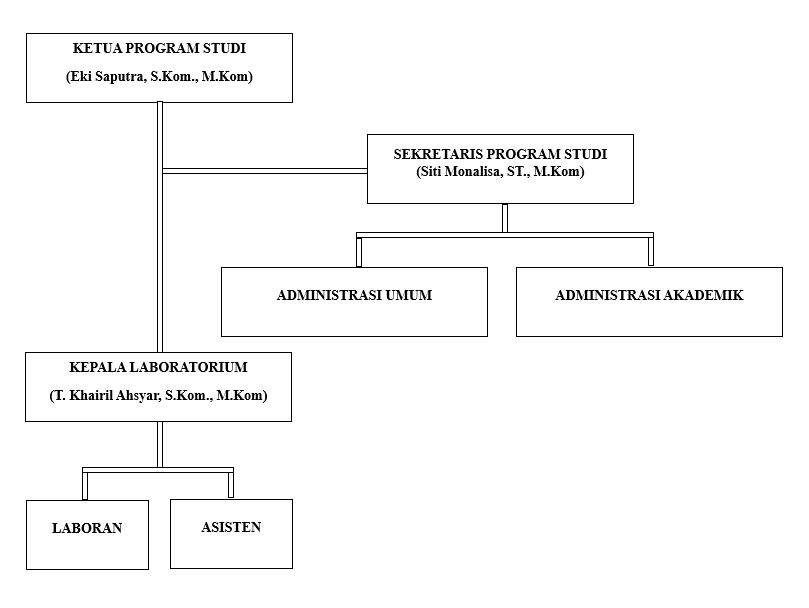
\includegraphics[width=0.82\linewidth]{konten//gambar/Struktur Organisasi.png}
  \caption{Struktur Organisasi Laboratorium}
  \label{fig:enter-label}
\end{figure}
% \subsection{a}
% % -----------------------------------------------------------------------------%
% \subsection{a}
% % -----------------------------------------------------------------------------%
% \begin{enumerate}
% 	\item Isi sesuai keinginan
% \end{enumerate}
% % -----------------------------------------------------------------------------%
% \section{Sistem}
% % -----------------------------------------------------------------------------%
% Sistem adalah suatu jaringan kerja dari prosedur-prosedur yang saling berhubungan, berkumpul bersama-sama untuk melakukan suatu kegiatan atau menyelesaikan suatu sasaran tertentu (Ahmad dan Hasti, 2018). Sistem juga bisa diartikan sebagai kesatuan bagian-bagian yang saling berhubungan yang berada dalam suatu wilayah serta memiliki item-item penggerak, dan bisa diartikan menjadi sangat luas, pada bidang computer fungsi sistem tersebut dapat berupa media untuk melakukan input, proses, dan output (hasil) dari suatu data \cite{audrilia2020perancangan}
% -----------------------------------------------------------------------------%
% \section{Informasi}
% Informasi merupakan hasil dari pengolahan data sehingga menjadi bentuk yang penting bagi penerimanya dan mempunyai kegunaan sebagai dasar dalam pengambilan keputusan yang dapat dirasakan akibatnya secara langsung saat itu juga atau secara tidak langsung pada saat mendatang \cite{henny2020sistem}. Dalam arti lain informasi adalah data yang diolah menjadi bentuk yang lebih berguna berarti bagi penggunanya \cite{audrilia2020perancangan}
% -----------------------------------------------------------------------------%

\section{Inventaris}
Inventaris merupakan sebuah kata yang diasimilasikan dari kata \textit{inventory} yang berasal dari bahasa Inggris. Echols dan Shadily merumuskan dalam kamus Besar Bahasa Indonesia sebagai daftar barang disertai dengan nilainya masing-masing yang dimilki perusahaan dalam kurun waktu tertentu yang digunakan dalam kegiatan usaha perusahaan. Dalam praktek, inventaris disebut juga sebagai persediaan barang yang artinya barang-barang biasanya dapat dijumpai digudang tertutup, lapangan, gudang terbuka atau tempat-tempat penyimpanan lain, baik berupa bahan baku, barang setengah jadi, barang jadi barang-barang untuk keperluan operasi atau barang-barang untuk keperluan suatu proyek \cite{novendri2019aplikasi}.
% -----------------------------------------------------------------------------%
\section{Sistem Informasi Inventaris}
% -----------------------------------------------------------------------------%
Sistem informasi adalah suatu sistem didalam Organisasi yang mempertemukan kebutuhan pengolahan transaksi harian, mendukung operasi bersifat manajerial dan kegiatan strategi dari suatu organisasi dan menyediakan pihak luar tertentu dengan laporan-laporan yang diperlukan \cite{laila2011sistem}. Sistem informasi inventaris adalah suatu sistem yang digunakan untuk mengelola dan memantau inventaris atau barang yang dimiliki oleh suatu organisasi atau perusahaan. Sistem ini dapat membantu memudahkan petugas inventaris dalam pendataan barang yang dimiliki oleh organisasi atau perusahaan tersebut \cite{Yanti2021SISTEMII}.
%-----------------------------------------------------------------------------%
%-----------------------------------------------------------------------------%
\section{Laboratorium}
Laboratorium merupakan sarana dalam melaksanakan sebuah riset dalam bidang ilmiah, eksperimen, pengukuran maupun pelatihan ilmiah. Meski laboratorium telah memiliki alat-alat yang lengkap, pengelolaan laboratorium juga harus diperhatikan. Adanya alat-alat yang sudah lengkap dan penggunaan yang sudah baik tentunya perlu untuk dilakukan manajemen yang baik pada laboratorium tersebut, karena terdapat beberapa hal yang harus diperhatikan kembali seperti pengelolaan masing-masing laboratorium dan pengolahan data \cite{sweden2022rancang}.
\subsection{Laboratorium Rekayasa Sistem Informasi (RSI)}
Laboratorium Rekayasa sistem Informasi atau yang disingkat dengan nama Laboratorium RSI merupakan laboratorium pertama yang dimiliki oleh Program Studi Sistem Informasi sejak pindahnya aktivitas perkuliahan kampus dari kampus Sukajadi ke kampus utama Panam Pekanbaru Riau pada tahun 2007. Fungsi utama dari laboratorium ini adalah sebagai fasilitas infrastruktur pendukung untuk pelaksanaan kegiatan perkuliahan praktikum bagi mahasiswa Program Studi Sistem Informasi terkait bidang Rekayasa Sistem Informasi. Bidang Rekayasa Sistem Informasi merupakan bidang yang paling dominan yang ada di Program Studi Sistem Informasi \cite{lab-si-website}.

\subsection{Laboratorium Internet (INT)}
Laboratorium Internet atau yang disingkat dengan nama Laboratorium INT merupakan laboratorium milik Program Studi Sistem Informasi di bawah Fakultas Sains dan Teknologi kedua yang aktivitas perkuliahannya berada di kampus utama Panam Pekanbaru Riau. Secara spesifik, laboratorium ini lebih dioperasikan untuk kebutuhan perkuliahan terkait matakuliah praktikum dasar, seperti matakuliah Jaringan Komputer dan Pemrograman Dasar \cite{lab-si-website}.

\subsection{Laboratorium \textit{Software Engineering} (SE)}
Laboratorium ke tiga yang dimiliki oleh Program Studi Sistem Informasi adalah Laboratorium \textit{Software Engineering} atau yang disingkat dengan nama Laboratorium SE. Laboratorium ini merupakan laboratorium terbaru milik yang dikelola oleh Program Studi dari usulan pengadaan barang tahun anggaran 2021 di bawah naungan Fakultas Sains dan Teknologi UIN Suska Riau. Adapun laboratorium SE sebagai pendukung dalam pelaksanaan kegiatan perkuliahan praktikum bagi mahasiswa Program Studi Sistem Informasi yang terkait dengan bidang keilmuan seperti Praktikum Basis Data, Pemrograman Beorientasi Objek (PBO), dan matakuliah wajib praktikum lainnya \cite{lab-si-website}.

%-----------------------------------------------------------------------------%
\section{Web}
Rangkaian jaringan yang tersebar di seluruh dunia, yang di semua organisasi dihubungkan oleh jaringan terbesar sehingga dapat saling berkomunikasi, adalah istilah internet. Dengan Internet, pengguna dapat mengakses berbagai sistem dari mana saja, internet juga sebagai penghubung jaringan website. \textit{World Wide Web} (WWW) atau Website adalah laman-laman berisikan keterangan yang berada dalam taraf global berbasis \textit{hypertext} yang memungkinkan pengguna mencari banyak sekali macam keterangan pada dunia selama terhubung menggunakan internet \cite{tyowati2017implementasi}.
%-----------------------------------------------------------------------------%
\section{\textit{Framework}}
\textit{Framework} dalam pengembangan sistem adalah kerangka kerja atau struktur yang digunakan untuk memudahkan pengembangan aplikasi atau sistem \cite{sallaby2020perancangan}. \textit{Framework} menyediakan berbagai fitur dan fungsi yang dapat digunakan oleh pengembang untuk mempercepat proses pengembangan dan memastikan konsistensi dalam pengembangan aplikasi atau sistem \cite{simanullang2021sistem}. \textit{Framework} juga membantu pengembang dalam mengelola kode program dan memperbaiki bug. Beberapa contoh \textit{framework} yang sering digunakan dalam pengembangan sistem adalah Laravel, CodeIgniter, dan beberapa \textit{framework} lainnya \cite{Fadllullah2022PengembanganSI}.
%-----------------------------------------------------------------------------%
\section{Codeigniter}
Codeigniter merupakan \textit{framework} untuk membangun aplikasi web berbasis PHP  Codeigniter menyediakan banyak \textit{library} untuk fungsi-fungsi umum, antar muka yang sederhana, dan struktur yang logis. CodeIgniter menjadi sebuah \textit{framework} PHP dengan model MVC \textit{(Model, View, Controller)} untuk membangun website dinamis dengan menggunakan PHP yang dapat mempercepat pengembang untuk membuat sebuah aplikasi web. Selain ringan dan cepat, CodeIgniter juga memiliki dokumentasi yang super lengkap disertai dengan contoh implementasi kodenya. Programmer dapat membuat aplikasi dengan lebih cepat karena tidak perlu menulis kode dari awal, selain itu Codeigniter juga menyediakan banyak fungsi yang siap digunakan. Seorang programmer bisa lebih fokus dengan aplikasi yang sedang dibangun dan meminimalkan penulisan kode \cite{tyowati2017implementasi}.
%-----------------------------------------------------------------------------%
\section{\textit{Database}}
\textit{Database} adalah suatu kumpulan data yang telah diatur secara terstruktur, memungkinkan akses dan pengelolaan melalui sistem komputer. Jenis data yang dapat disimpan di dalamnya mencakup teks, gambar, suara, dan video, dengan berbagai tujuan seperti penyimpanan informasi, analisis data, dan pengambilan keputusan. Untuk membuat dan mengelola \textit{database}, diperlukan perangkat lunak khusus seperti MariaDB, Oracle, atau Microsoft SQL Server \cite{Cowls2021ADB}.
%-----------------------------------------------------------------------------%
\section{MariaDB}
MariaDB sebenarnya merupakan turunan salah satu konsep utama dalam basis data yang telah ada sebelumnya SQL \textit{(Structured Query Language)}. SQL adalah sebuah konsep pengoperasian basis data, terutama untuk pemilihan atau seleksi dan pemasukan data yang memungkinkan pengoperasian data dikerjakan dengan mudah secara otomatis \cite{priyanti2013sistem}.
%-----------------------------------------------------------------------------%
\section{PHP}
\textit{Hypertext Preprocessor} (PHP) adalah pemrograman interpreter yaitu proses penerjemahan baris kode sumber menjadi kode mesin yang dimengerti komputer secara langsung pada saat baris kode dijalankan. PHP disebut sebagai pemrograman \textit{Server Side Programming}, hal ini dikarenakan seluruh proses nya dijalankan pada server. PHP adalah sebuah bahasa dengan hak cipta terbuka atau yang juga dikenal dengan istilah \textit{open source}, yaitu pengguna dapat mengembangkan kode-kode fungsi PHP sesuai dengan kebutuhannya \cite{php2001php}.
%-----------------------------------------------------------------------------%
\section{XAMPP}
XAMPP adalah sebuah paket lengkap untuk server web yang dapat dengan mudah diinstal di berbagai sistem operasi. Dalam paket ini sudah termasuk beberapa komponen penting seperti Apache (web server), MariaDB \textit{(database)}, PHP (server side scripting), dan berbagai pustaka pendukung lainnya. XAMPP dapat digunakan pada berbagai sistem operasi, termasuk Linux, Windows, MacOS, dan Solaris, sehingga memudahkan pembuatan server web \textit{multi-platform} \cite{pakpahan2020sistem}.
%-----------------------------------------------------------------------------%
%-----------------------------------------------------------------------------------------------%
%
% % Oktober 2022
% Template Latex untuk Laporan Kerja Praktek Program Studi Sistem informasi ini
% Dikembangkan oleh Daffa Takratama Savra (daffatakratama13@gmail.com)

% Template ini dikembangkan dari template yang dibuat oleh Inggih Permana (inggihjava@gmail.com).

% Orang yang cerdas adalah orang yang paling banyak mengingat kematian.
%
%-----------------------------------------------------------------------------------------------%


%-----------------------------------------------------------------------------%
\chapter{\babTiga}
%-----------------------------------------------------------------------------%
\section{Waktu dan Tempat Pelaksaan Kerja Praktek}
Waktu	: Tanggal 03 Juli sampai dengan tanggal 01 September 2023

Tempat: Laboratorium Prodi Sistem Informasi

Alamat	: Jl. Soebrantas No. 155 KM 15, Pekanbaru 28293

%-----------------------------------------------------------------------------%
\subsection{Jadwal Kerja Praktek}
Pelaksanaan kegiatan dilakukan dalam kurun waktu 2 (dua) bulan terhitung sejak tanggal 03 Juli – 01 September tahun 2023. Jadwal kerja praktek dapat dilihat pada Gambar 3.1 berikut:

\begin{figure}
  \centering
  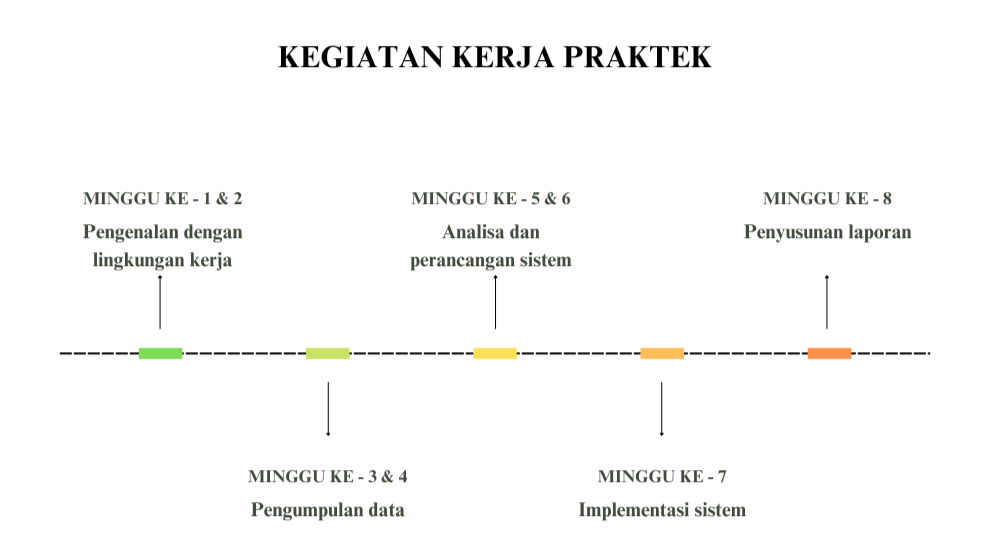
\includegraphics[width=0.82\linewidth]{konten//gambar/kegiatan kerja praktek.png}
  \caption{Kegiatan Kerja Praktek}
  \label{fig:enter-label}
\end{figure}
%-----------------------------------------------------------------------------%
\subsection{Uraian Kerja Praktek}
%-----------------------------------------------------------------------------%
Tugas kerja praktek ini dilaksanakan pada Laboratorium Sistem Informasi
UIN Suska Riau yang beralamatkan Jl. H.R. Soebrantas KM 15, Tuah Madani, Panam, Pekanbaru dalam kurun waktu 58 hari dihitung sejak 03 Juli 2023 sampai 01 September 2023. Kegiatan yang dilakukan disusun dalam proses perencanaan kerja, rencana tersebut adalah:
\begin{enumerate}
  \item Kegiatan pada minggu pertama dan kedua dilakukan agenda proses perkenalan dengan pegawai dan pembimbing kerja praktek di tempat kerja praktek. Perkenalan dilakukan pada tanggal 03 Juli 2023 mulai dari memperkenalkan diri kepada pegawai di tempat kerja praktek.
  \item Pada minggu ketiga dan keempat dilakukan proses pengamatan alur dan prosedur kerja, serta sudah mulai melakukan pengumpulan data dan pengolahan data dengan melakukan teknik pengumpulan seperti observasi dan wawancara yang di khususkan mengenai analisis dan perancangan sistem informasi.
  \item Pada minggu keempat dan kelima dilakukan proses analisa kebutuhan sistem yang diperlukan dari data yang diperoleh.
  \item Selanjutnya pada minggu keenam, ketujuh dan kedelapan yaitu melanjutkan perancangan dan sudah masuk ketahap pengkodingan dan implementasi sistem, sekaligus merupakan minggu perpisahan pada kerja praktek.
\end{enumerate}
%-----------------------------------------------------------------------------%
\section{Metodologi Kerja Praktek}
Metodologi berisi tahapan-tahapan yang dilakukan dalam penyusunan lapo-
ran kerja praktek. langkah – langkah yang ditempuh dalam melakukan penelitian ini
dapat dilihat pada Gambar 3.2 berikut.
\begin{figure}
  \centering
  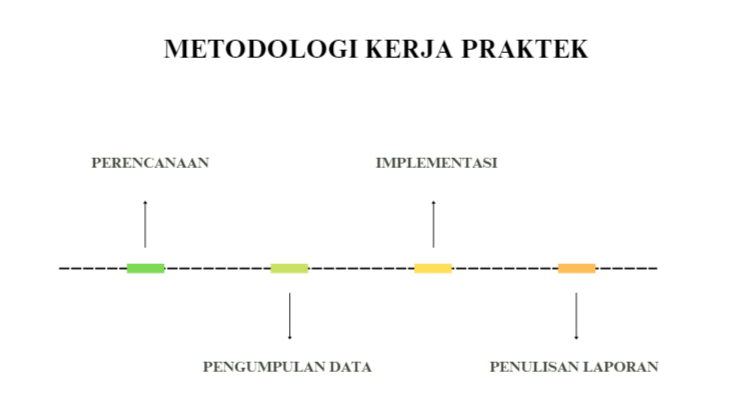
\includegraphics[width=0.82\linewidth]{konten//gambar/metodologi kerja praktek.png}
  \caption{Metodologi Kerja Praktek}
  \label{fig:enter-label}
\end{figure}
%-----------------------------------------------------------------------------%
% Isi sesuai keinginan
%-----------------------------------------------------------------------------%
\subsection{Tahap Perencanaan }
%-----------------------------------------------------------------------------%
Langkah pertama adalah menetapkan masalah yang akan dipecahkan, adapun langkah-langkah dalam perencanaan sebagai berikut:
\begin{enumerate}
  \item Mulai \\
        Merupakan tahapan awal dalam setiap kegiatan yang akan dilakukan.
  \item Menentukan Topik Penelitian \\
        Topik penelitian ditentukan dari uraian masalah dan kendala yang didapat dari observasi secara langsung di Laboratorium Sistem Informasi.
  \item Menentukan Masalah \\
        Setelah observasi dilakukan, untuk mendukung pencapaian kerja praktek ini maka selanjutnya dilakukan penentuan masalah agar bisa mendapat masalah untuk dipecahkan.
  \item Menentukan Tujuan Kerja Praktek \\
        Selanjutnya adalah penentuan tujuan dari Kerja Praktek ini, agar tujuan dalam penulisan Laporan Kerja Praktek lebih Jelas.
  \item Menentukan Metode Penelitian \\
        Agar hasil dari penelitian ini sesuai harapan maka dibutuhkan penentuan implementasi untuk mendukung penelitian ini yaitu menggunakan \textit{framework} CodeIgniter 4.
\end{enumerate}
%-----------------------------------------------------------------------------%
\subsection{Tahap Pengumpulan Data}
%-----------------------------------------------------------------------------%
Tahap ini adalah tahap penulis melaksanakan pengumpulan data Kerja Praktek, pada tahap ini yang dilakukan adalah:
\begin{enumerate}
  \item  Observasi \\
        Penulis melakukan pengamatan di Laboratorium Sistem Informasi secara langsung.
  \item  Wawancara \\
        Penulis melakukan wawancara langsung dengan Kepala Laboratorium Sistem Informasi UIN Suska Riau untuk mengajukan beberapa pertanyaan.
        % \item  Studi Pustaka \\
        % Studi pustaka dilakukan dengan cara mengambil literature yang berkaitan dengan materi. Pada tahapan pengumpulan data studi pustaka Penulis mengambil beberapa referensi dari buku, jurnal, ebook dan internet.
\end{enumerate}

% Data yang dikumpulkan adalah sebagai berikut:
% \begin{enumerate}
%     \item Data Primer \\
%     Data Primer adalah data yang diambil secara langsung dari sumber aslinya, melalui narasumber yang tepat dan dapat dijadikan data pembuatan laporan.
%     \item Sekunder
%     Data Sekunder adalah data yang diambil melalui jurnal, e-book dan juga buku-buku referensi dari berbagai penulis.
% \end{enumerate}
%-----------------------------------------------------------------------------%
% \subsection{Tahap Analisa dan Hasil}
% %-----------------------------------------------------------------------------%
% Tahap analisa dan perancangan dilakukan untuk membuat rancangan sistem yang baru dengan menganalisa data-data yang sudah didapatkan dari hasil pengumpulan data sebelumnya.
% \begin{enumerate}
%       \item Analisa sistem lama \\
%             Berdasarkan data-data yang telah didapatkan pada tahap pengumpulan data, maka dilakukan analisa sistem yang digunakan dalam proses pencatatan inventaris dimulai dari permasalahan yang terjadi saat proses pencatatan, peminjaman, dan cara mengatasi permasalahan yang terjadi.
%       \item Analisa sistem baru \\
%             Dari analisa sistem lama, maka dilakukan analisa dan rancangan sistem baru untuk mengatasi permasalahan dengan mengunakan metode yang dipilih pada tahapan perencanaan.
% \end{enumerate}
%-----------------------------------------------------------------------------%
\subsection{Tahap Implementasi}
%-----------------------------------------------------------------------------%
Pada tahap implementasi dilakukan pengkodingan untuk membangun sistem yang sudah dianalisa dan dirancang pada tahap sebelumnya.
\begin{enumerate}
  \item Mengimplementasikan sistem informasi inventaris laboratorium melanjutkan desain \textit{interface}, \textit{database}, dan UML yang sudah dilakukan pada tahap sebelumnya yang akan digunakan sebelum tahap pengkodingan.
  \item Melakukan kodingan sistem
        Melakukan pengkodingan sistem inventaris dengan rancangan yang telah dibuat dengan desain-desain yang telah dibuat sebelumnya.
\end{enumerate}
%-----------------------------------------------------------------------------%
\subsection{Tahap Penulisan Laporan}
%-----------------------------------------------------------------------------%
Tahap terakhir ini adalah melakukan penulisan laporan. Kegiatan yang dilakukan diantaranya melakukan konsultasi terhadap pembimbing, dokumentasi hasil kerja praktek hingga selesainya penulisan laporan.
%-----------------------------------------------------------------------------%

\ifthenelse{\equal{\bidangta}{DUA}}{
  \renewcommand{\babEmpat}{HASIL IMPLEMENTASI}
  \renewcommand{\babLima}{PENUTUP}
}{}

\ifthenelse{\equal{\tipeta}{LAPORAN KERJA PRAKTEK}}{
  \renewcommand{\babEmpat}{HASIL IMPLEMENTASI}
}{}

%-----------------------------------------------------------------------------------------------%
%
% % Oktober 2022
% Template Latex untuk Laporan Kerja Praktek Program Studi Sistem informasi ini
% Dikembangkan oleh Daffa Takratama Savra (daffatakratama13@gmail.com)

% Template ini dikembangkan dari template yang dibuat oleh Inggih Permana (inggihjava@gmail.com).

% Orang yang cerdas adalah orang yang paling banyak mengingat kematian.
%
%-----------------------------------------------------------------------------------------------%


%-----------------------------------------------------------------------------%
\chapter{\babEmpat}
% -----------------------------------------------------------------------------%
\section{Analisa Sistem}
% -----------------------------------------------------------------------------%
Analisa sistem merupakan kegiatan penguraian suatu sistem informasi yang utuh dan nyata ke dalam bagian-bagian atau komponen-komponen komputer yang bertujuan untuk mengidentifikasi serta mengevaluasi masalah-masalah yang muncul, hambatan-hambatan yang mungkin terjadi, serta kebutuhan yang diharapkan, sehingga dapat memberikan suatu solusi untuk perbaikan maupun pengembangan ke arah yang lebih baik dan sesuai dengan kebutuhan serta perkembangan teknologi \cite{nugraha2014analisa}. Pada tahap analisis sistem dilakukan beberapa proses yang berhubungan dengan tahap awal metode penelitian, pada analisa dan perancangan sistem ini dilakukan oleh Nasya Amirah Melyani 2023 pada penelitian sebelumnya.
% dan diimplementasikan dalam \textit{framework} CodeIgniter 4.
% \subsection{Analisa Sistem yang Sedang Berjalan}
Setelah dilakukan analisa dan perancangan pada penelitian sebelumnya, maka dilakukan sebuah implementasi sistem yang terintegrasi dalam sebuah \textit{database} untuk proses pengelolaan inventaris. Sistem informasi yang dibangun ini nantinya diharapkan mampu memberikan kemudahan dalam pengelolaan barang inventaris di Laboratorium Sistem Informasi.
% Berikut adalah uraian dari sistem yang sedang berjalan di laboratorium Sistem Informasi:
% \begin{enumerate}
%   \item Proses pencatatan barang-barang Inventaris seperti komputer, mouse, keyboard, dll. Masih dilakukan secara manual dan konvensional.
%   \item Proses pengkodean barang masih dilakukan secara biasa dan belum seperti kaidah pengkodean semestinya.
%   \item Proses Pengelolaan data dan laporan masih dilakukan secara manual dan konvensional yang tidak efektif dan efisien.
% \end{enumerate}

% -----------------------------------------------------------------------------%
\section{Rencana Sistem yang Usulan}
% -----------------------------------------------------------------------------%
Setelah dilakukan analisa dan perancangan pada penelitian sebelumnya, maka dilaksanakan sebuah implementasi sistem yang terintegrasi dalam sebuah \textit{database} untuk proses pengelolaan inventaris. Sistem informasi yang dibangun ini nantinya diharapkan mampu memberikan kemudahan dalam pencatatan barang inventaris laboratorium serta memberikan kemudahan dalam melihat laporan terkait barang berdasarkan lokasi, pendanaan, kategori dan tahun. Adapun rancangan sistem usulan ini memiliki beberapa kelebihan, sebagai berikut:

\begin{enumerate}
  \item Barang yang masuk bisa terdata dengan baik dan memudahkan petugas dalam melakukan pencatatan.
  \item Melakukan pengkodean terhadap barang laboratorium.
  \item Tidak adanya barang yang tidak terdata pada Laboratorium Sistem Informasi.
  \item Mempermudah Laboratorium Prodi Sistem Informasi dalam proses rekapitulasi laporan inventaris barang.
\end{enumerate}

Berdasarkan hasil analisis dan perancangan pada penelitian sebelumnya, maka dapat dilakukan implementasi sistem informasi Inventaris pada Laboratorium Sistem Informasi, dengan menggunakan pendekatan berorientasi objek dan menggunakan \textit{framework} CodeIgniter 4 dengan konsep Model, \textit{View}, dan \textit{Controller}.

Implementasi sistem akan memberikan kemudahan dalam memberikan penjelasan komprehensif dan gambaran lengkap mengenai bentuk serta rancangan kerja dari sistem tersebut. Hal ini sangat penting dalam memastikan bahwa sistem yang diusulkan dapat memenuhi kebutuhan operasional instansi dengan efisien dan efektif. Ini membantu pihak terkait, termasuk Laboratorium Prodi Sistem Informasi, untuk memahami secara mendalam bagaimana sistem akan beroperasi dan bagaimana barang inventaris akan dicatat dan dikelola.

% -----------------------------------------------------------------------------%
% \subsection{\textit{Use Case Diagram}}
% % -----------------------------------------------------------------------------%
% \subsection{\textit{Activity Diagram}}
% % -----------------------------------------------------------------------------%
% \subsection{\textit{Sequence Diagram}}
% % -----------------------------------------------------------------------------%
% \subsection{\textit{Class Diagram}}
% % -----------------------------------------------------------------------------%
% \subsection{Perancangan Basis Data}
% % -----------------------------------------------------------------------------%
% \subsection{Perancangan \textit{Interface}}
% -----------------------------------------------------------------------------%
\section{Implementasi Sistem}
% -----------------------------------------------------------------------------%
Implementasi adalah tahap repersentasi perangkat lunak sesuai dengan hasil analisa yang telah dilakukan \cite{huda2022implementasi}. Implementasi perlu dilakukan bertujuan untuk menjelaskan modul kepada \textit{user} dalam menggunakan aplikasi. Sehingga \textit{user} dapat merespon aplikasi yang dibangun untuk memberikan masukan-masukan agar aplikasi dapat dikembangkan menjadi lebih baik lagi.
% -----------------------------------------------------------------------------%
\section{Batasan Implementasi}
Batasan implementasi Sistem Informasi Inventaris Laboratorium (SITARIS) dalam penelitian untuk Kerja Praktek ini adalah:
\begin{enumerate}
  \item Sistem yang dibangun memiliki \textit{platform} berbasis\textit{ Web}.
  \item Sistem yang dibangun memiliki hak akses seperti Admin, Kalab, Kaprodi, Sekprodi, dan Aslab. Dosen dan Mahasiswa dapat menggunakan fitur yang disediakan sesuai hak akses masing-masing.
  \item Menggunakan bahasa pemrograman PHP dengan \textit{framework} CodeIgniter dan \textit{database} MariaDB/PHPMyadmin.
  \item Sistem dapat menampilkan data barang, pendanaan, dokumentasi, peminjaman barang, peminjaman ruangan, \textit{maintenance}, pemusnahan barang, fakultas/lembaga, program studi/unit, gedung, ruangan, dan pengguna.
\end{enumerate}
% -----------------------------------------------------------------------------%
\section{Implementasi Perangkat Keras (\textit{Hardware})}
% -----------------------------------------------------------------------------%
% Implementasi pada lingkungan \textit{hardware} adalah implementasi pada perangkat keras yang digunakan untuk menjalankan sistem informasi inventaris laboratorium. Implementasi \textit{hardware} yang digunakan dapat dilihat pada Tabel 4.1.

Minimum kebutuhan pada implementasi hardware untuk menjalankan sistem informasi inventaris laboratorium adalah spesifikasi perangkat keras yang harus terpenuhi agar sistem dapat beroperasi secara optimal. Tabel 4.1. menyajikan daftar rinci dari komponen perangkat keras yang diperlukan dan spesifikasinya, yang mencakup prosesor, RAM, Hardisk, Monitor, dan perangkat masukan yang harus memenuhi standar minimum agar sistem berfungsi dengan baik.

\begin{table}[h]
  \centering
  \caption{Spesifikasi Perangkat Keras (\textit{Hardware})}
  \begin{tabular}{|l|l|}
    \hline
    \textbf{Komponen \textit{Hardware}} & \textbf{Spesifikasi}            \\ \hline
    Processor                           & Intel ® CoreTM i3-4160, 3.60GHz \\ \hline
    Memory (RAM)                        & 2 GB                            \\ \hline
    Hardisk (HDD)                       & 1 TB                            \\ \hline
    LCD                                 & Lenovo 17”                      \\ \hline
  \end{tabular}
\end{table}

\section{Implementasi Perangkat Lunak (\textit{Software})}
% -----------------------------------------------------------------------------%
Implementasi pada lingkungan \textit{software} adalah implementasi pada perangkat lunak yang digunakan untuk menjalankan sistem informasi inventaris laboratorium. Implementasi \textit{software} yang digunakan dapat dilihat pada Tabel 4.2.

\begin{table}[h]
  \centering
  \caption{Spesifikasi Perangkat Lunak (\textit{Software})}
  \begin{tabular}{|l|l|}
    \hline
    \textbf{Komponen \textit{Software}} & \textbf{Spesifikasi}              \\ \hline
    Sistem Operasi                      & Windows 7, 8, 10, dan 11          \\ \hline
    Browser                             & Google Chrome dan Mozilla Firefox \\ \hline
    Bahasa Pemrograman                  & PHP dan Javascript                \\ \hline
    Web \textit{Database}               & MariaDB                           \\ \hline
    \textit{Framework}                  & CodeIgniter 4                     \\ \hline
  \end{tabular}
\end{table}
% -----------------------------------------------------------------------------%
\section{Implementasi Basis Data (\textit{Database})}
Pada penelitian sebelumnya sudah dilakukan perancangan \textit{database} oleh Nasya Amirah Melyani pada tahap Analisa dan Perancangan Sistem Informasi Inventaris Menggunakan Metode OOAD. Pada tahap implementasi ini, pembuatan \textit{database} dilakukan dengan menggunakan \textit{database} MariaDB. Berikut merupakan tampilan \textit{database} sistem inventaris laboratorium:
\begin{enumerate}
  \item \textit{Database} Sistem informasi inventaris laboratorium bernama mab\_lab. \textit{Database} sistem informasi inventaris laboratorium terdiri dari 15 tabel yaitu, tabel barang, tabel dokumentasi, tabel fakultas, tabel gedung, tabel \textit{maintenance}, tabel peminjaman\_barang, tabel peminjaman\_ruangan, tabel pemusnahan\_barang, tabel pendanaan, tabel prodi, tabel referensi, tabel ruangan, dan tabel user. Tampilan \textit{database} dapat dilihat pada Gambar 4.1.

        \begin{figure}
          \centering
          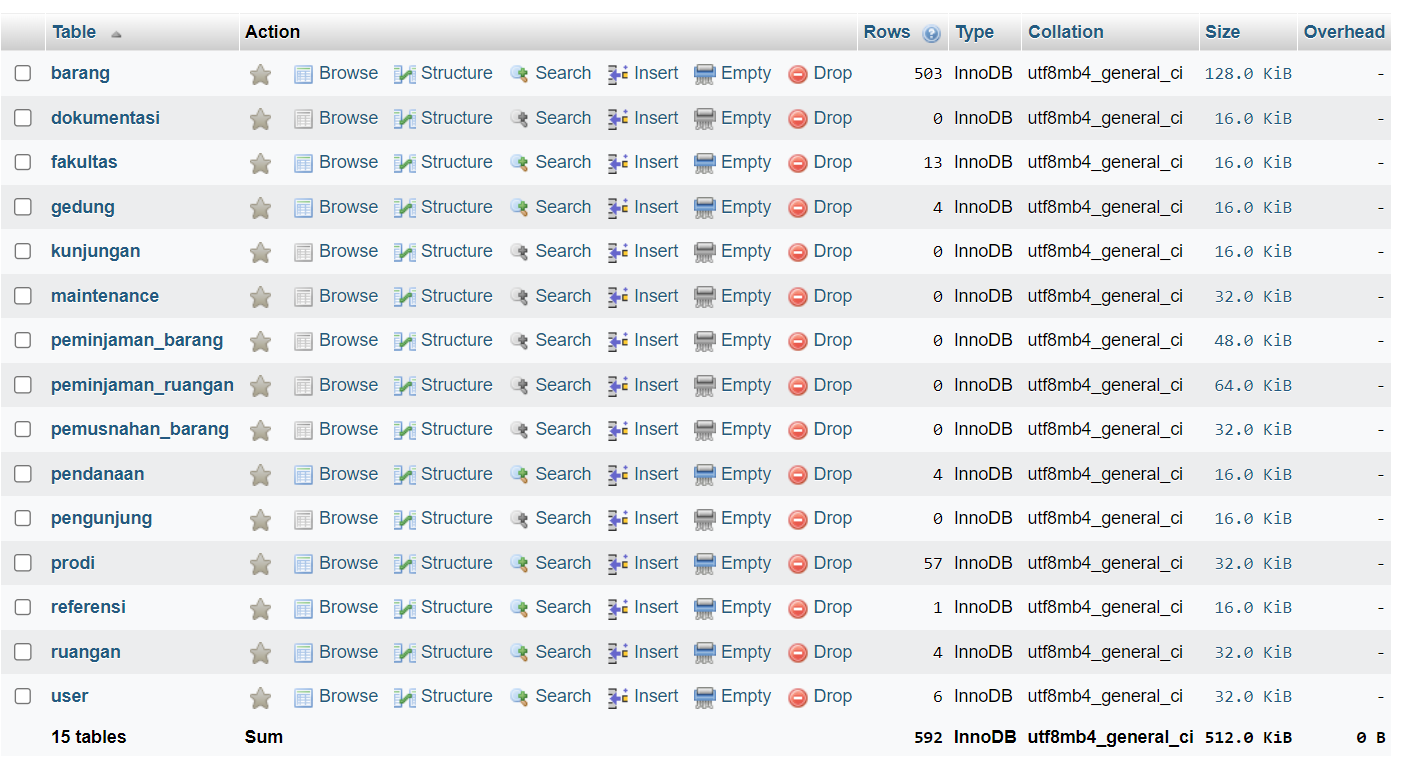
\includegraphics[width=0.82\linewidth]{konten//gambar/Tampilan tabel-tabel database.png}
          \caption{Tampilan Tabel Dalam \textit{Database}}
          \label{fig:enter-label}
        \end{figure}

  \item Struktur Tabel Barang
        Pada tabel data barang terdiri dari kolom id\_barang yang menjadi kunci utama dari tabel tersebut yang digunakan sebagai penanda agar tidak terjadi duplikasi data, id\_pendanaan menjadi kunci asing dalam tabel barang karena jenis pendanaan diperlukan dalam pencatatan data barang, id\_ruangan juga merupakan kunci asing yang diperoleh dari tabel ruangan karena nama ruangan diperlukan dalam pencatatan data barang, nama\_barang adalah kolom yang menyimpan nama barang yang dicatat, spek\_barang menjadi kolom yang menyimpan tentang spesifikasi barang yang dicatat, gambar\_barang merupakan kolom untuk menyimpan data gambar dari barang yang dicatat, tahun\_barang adalah kolom yang digunakan untuk mencatat tahun masuknya barang, kategori\_barang menjadi kolom untuk menyortir barang berdasarkan kategori, sub\_kategori menjadi kolom untuk menyortir barang berdasarkan subkategori turunan dari kategori barang, kondisi adalah kolom untuk menyimpan kondisi terakhir barang, tgl\_masuk\_barang digunakan untuk mengetahui tanggal masuknya barang atau tanggal dicatatnya barang, waktu\_input untuk mendeteksi kapan waktu dicatatnya barang, deskripsi menjelaskan lebih detail tentang barang yang dicatat, user\_input adalah kolom untuk melacak perubahan data berdasarkan siapa yang mencatat ke dalam sistem, user\_edit adalah kolom untuk melacak perubahan data berdasarkan siapa yang mengedit data dalam sistem, tgl\_edit adalah kolom untuk melacak perubahan data berdasarkan tanggal berapa data tersebut diedit. Tampilan dapat dilihat pada Gambar 4.2.

        \begin{figure}
          \centering
          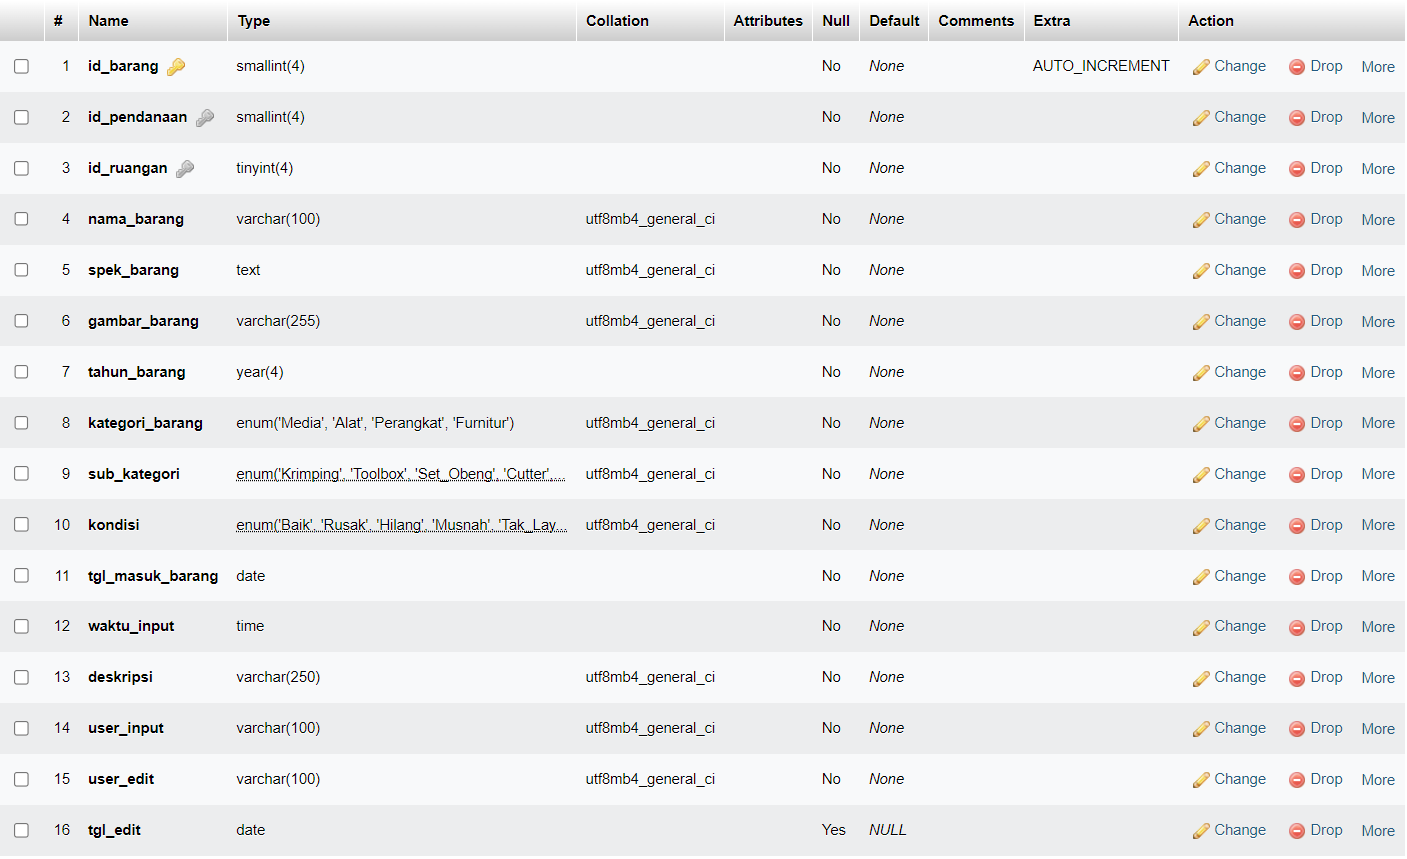
\includegraphics[width=0.82\linewidth]{konten//gambar/Tampilan database tabel barang.png}
          \caption{Tampilan \textit{Database} Tabel barang}
          \label{fig:enter-label}
        \end{figure}

  \item Struktur Tabel Dokumentasi
        Pada tabel data dokumentasi terdiri dari kolom id\_file yang menjadi kunci utama dari tabel tersebut yang digunakan sebagai penanda agar tidak terjadi duplikasi data, kategori\_dokumentasi menjadi kolom untuk menyortir dokumentasi berdasarkan kategori, nama\_dokumentasi adalah kolom yang menyimpan nama dokumentasi yang dicatat, deskripsi menjelaskan lebih detail tentang dokumentasi yang dicatat,  upload\_dokumentasi merupakan kolom untuk menyimpan data gambar atau dokumen dari dokumentasi yang dicatat, tgl\_upload digunakan untuk mengetahui tanggal diinputnya dokumentasi, waktu\_upload untuk mendeteksi kapan waktu diinputnya dokumentasi, user\_upload adalah kolom untuk melacak perubahan data berdasarkan siapa yang mencatat ke dalam sistem. Tampilan dapat dilihat pada Gambar 4.3.

        \begin{figure}
          \centering
          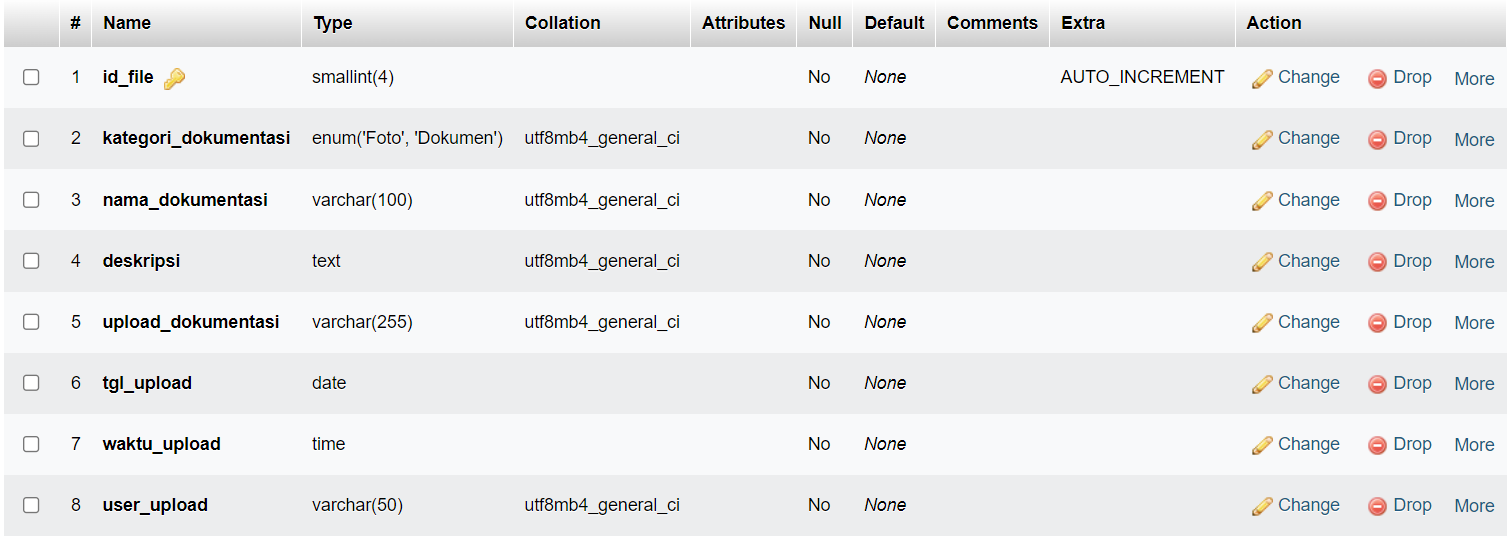
\includegraphics[width=0.82\linewidth]{konten//gambar/Tampilan database tabel dokumentasi.png}
          \caption{Tampilan \textit{Database} Tabel dokumentasi}
          \label{fig:enter-label}
        \end{figure}

  \item Struktur Tabel Fakultas
        Pada tabel data fakultas terdiri dari kolom id\_fakultas yang menjadi kunci utama dari tabel tersebut yang digunakan sebagai penanda agar tidak terjadi duplikasi data, nama\_fakultas adalah kolom yang menyimpan nama fakultas yang dicatat. Tampilan dapat dilihat pada Gambar 4.4.

        \begin{figure}
          \centering
          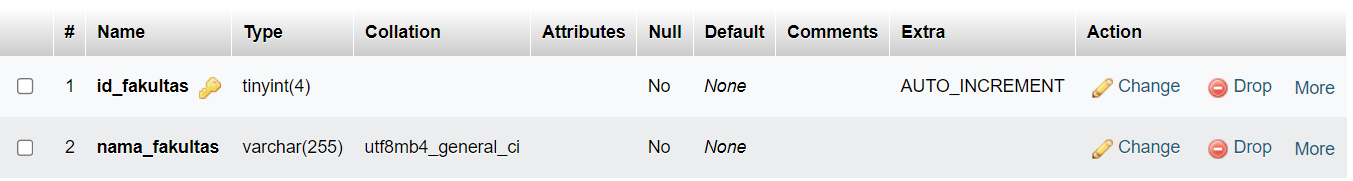
\includegraphics[width=0.82\linewidth]{konten//gambar/Tampilan database tabel fakultas.png}
          \caption{Tampilan \textit{Database} Tabel fakultas}
          \label{fig:enter-label}
        \end{figure}

  \item Struktur Tabel Gedung
        Pada tabel data gedung terdiri dari kolom id\_gedung yang menjadi kunci utama dari tabel tersebut yang digunakan sebagai penanda agar tidak terjadi duplikasi data, nama\_gedung adalah kolom yang menyimpan nama gedung yang dicatat,  deskripsi\_gedung menjelaskan lebih detail tentang gedung yang dicatat, gambar\_gedung merupakan kolom untuk menyimpan data gambar dari gedung yang dicatat. Tampilan dapat dilihat pada Gambar 4.5.

        \begin{figure}
          \centering
          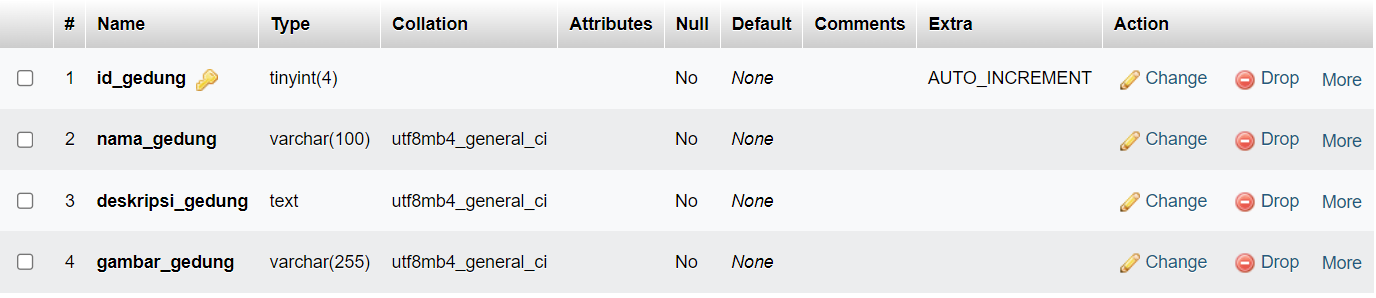
\includegraphics[width=0.82\linewidth]{konten//gambar/Tampilan database tabel gedung.png}
          \caption{Tampilan \textit{Database} Tabel gedung}
          \label{fig:enter-label}
        \end{figure}

  \item Struktur Tabel \textit{Maintenance}
        Pada tabel data \textit{maintenance} terdiri dari kolom id\_maintenance yang menjadi kunci utama dari tabel tersebut yang digunakan sebagai penanda agar tidak terjadi duplikasi data, id\_barang menjadi kunci asing dalam tabel \textit{maintenance} karena nama barang diperlukan dalam pencatatan data \textit{maintenance}, tgl\_maintenance digunakan untuk mengetahui tanggal dilakukannya \textit{maintenance} barang, kategori\_maintenance menjadi kolom untuk menyortir \textit{maintenance} berdasarkan kategori, biaya untuk menyimpan data biaya \textit{maintenance}, deskripsi menjelaskan lebih detail tentang \textit{maintenance} yang dilakukan, bukti merupakan kolom untuk menyimpan bukti \textit{maintenance} berupa gambar atau dokumen, status adalah kolom yang menyimpan data status \textit{maintenance} berupa sedang proses atau sudah selesai. Tampilan dapat dilihat pada Gambar 4.6.

        \begin{figure}
          \centering
          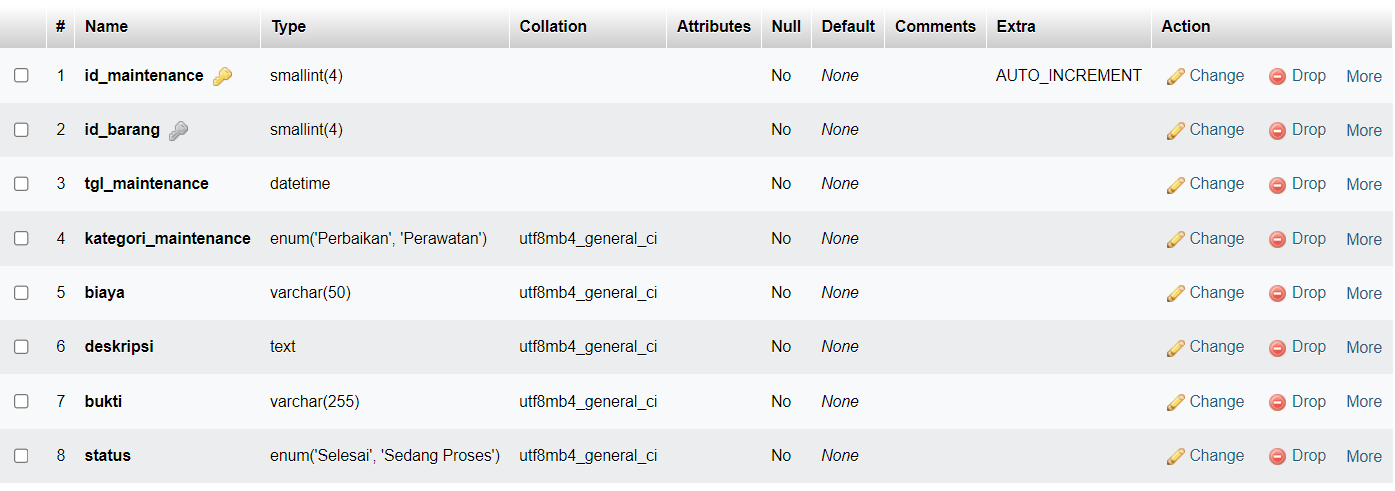
\includegraphics[width=0.82\linewidth]{konten//gambar/Tampilan database tabel maintenance.png}
          \caption{Tampilan \textit{Database} Tabel \textit{maintenance}}
          \label{fig:enter-label}
        \end{figure}

  \item Struktur Tabel Peminjaman Barang
        Pada tabel data peminjaman\_barang terdiri dari kolom id\_peminjaman\_barang yang menjadi kunci utama dari tabel tersebut yang digunakan sebagai penanda agar tidak terjadi duplikasi data, id\_barang, id\_fakultas menjadi kunci asing dalam tabel peminjaman barang karena nama fakultas diperlukan dalam pencatatan data peminjaman barang, id\_prodi menjadi kunci asing dalam tabel peminjaman barang karena nama prodi diperlukan dalam pencatatan data peminjaman barang, tgl\_peminjaman merupakan kolom untuk menyimpan tanggal barang dipinjam, tgl\_pengembalian merupakan kolom untuk menyimpan tanggal barang dikembalikan, asal\_peminjam merupakan kolom untuk membedakan antara peminjam internal dan peminjam eksternal, organisasi merupakan kolom untuk menyimpan nama organisasi dari peminjam, nama\_peminjam merupakan kolom untuk menyimpan nama dari peminjam, email\_peminjam merupakan kolom untuk menyimpan email dari peminjam, no\_hp merupakan kolom untuk menyimpan nomor telepon dari peminjam eksternal, bukti\_peminjaman merupakan kolom untuk menyimpan dokumen surat peminjaman, biaya\_peminjaman merupakan kolom untuk menampilkan biaya peminjaman pada peminjam eksternal, keterangan merupakan kolom untuk menyimpan data keperluan peminjaman yang diajukan oleh peminjam. Tampilan dapat dilihat pada Gambar 4.7.

        \begin{figure}
          \centering
          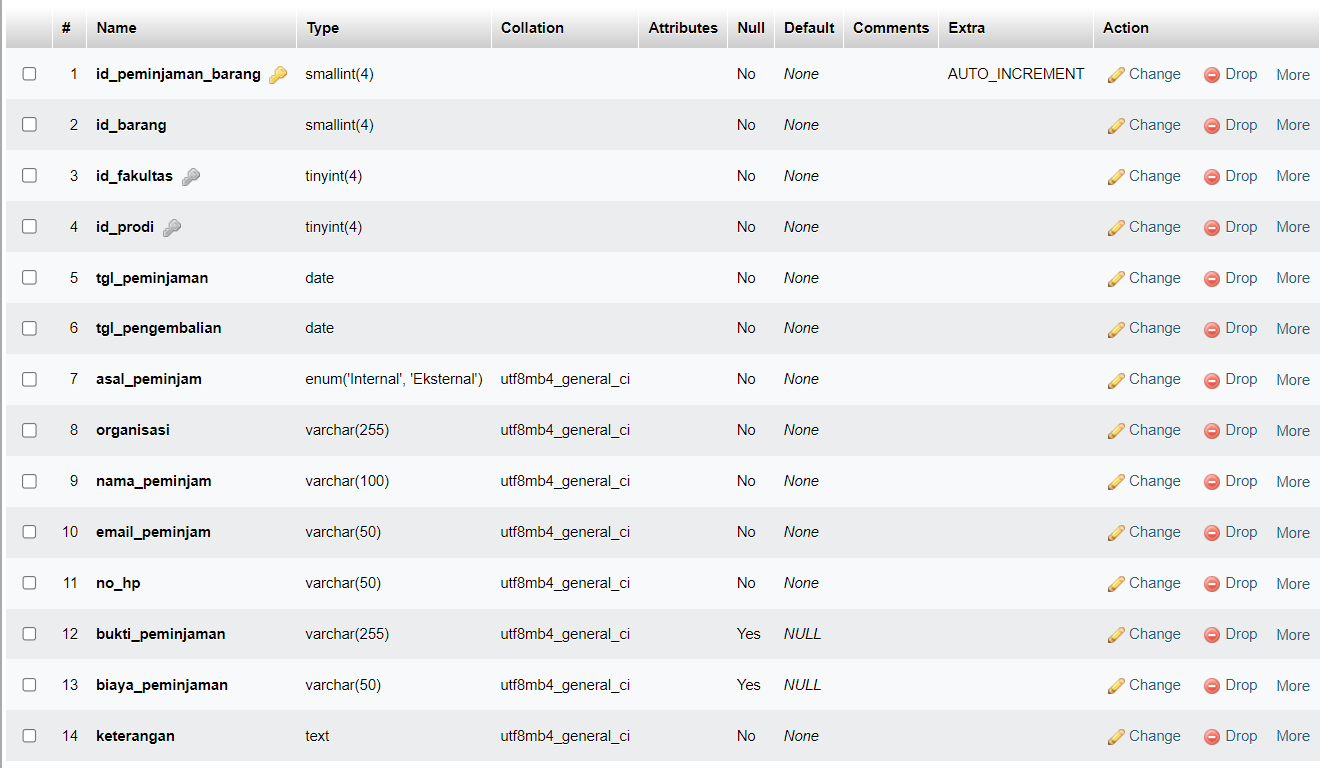
\includegraphics[width=0.82\linewidth]{konten//gambar/Tampilan database tabel peminjaman_barang.png}
          \caption{Tampilan \textit{Database} Tabel peminjaman\_barang}
          \label{fig:enter-label}
        \end{figure}

  \item Struktur Tabel Peminjaman Ruangan
        Pada tabel data peminjaman\_ruangan terdiri dari kolom id\_peminjaman\_ruangan yang menjadi kunci utama dari tabel tersebut yang digunakan sebagai penanda agar tidak terjadi duplikasi data,	id\_fakultas menjadi kunci asing dalam tabel peminjaman ruangan karena nama fakultas diperlukan dalam pencatatan data peminjaman ruangan,	id\_prodi menjadi kunci asing dalam tabel peminjaman ruangan karena nama prodi diperlukan dalam pencatatan data peminjaman ruangan,	id\_ruangan menjadi kunci asing dalam tabel peminjaman ruangan karena nama ruangan diperlukan dalam pencatatan data peminjaman ruangan yang akan dipinjam, asal\_peminjam merupakan kolom untuk membedakan antara peminjam internal dan peminjam eksternal,	organisasi merupakan kolom untuk menyimpan nama organisasi dari peminjam,	nama\_peminjam merupakan kolom untuk menyimpan nama dari peminjam, email\_peminjam merupakan kolom untuk menyimpan email dari peminjam, no\_hp merupakan kolom untuk menyimpan nomor telepon dari peminjam eksternal, tgl\_peminjaman merupakan kolom untuk menyimpan tanggal ruangan dipinjam, lama\_peminjaman merupakan kolom untuk menyimpan lama ruangan dipinjam,	biaya\_peminjaman merupakan kolom untuk menampilkan biaya peminjaman pada peminjam eksternal, bukti\_peminjaman merupakan kolom untuk menyimpan dokumen surat peminjaman, keterangan merupakan kolom untuk menyimpan data keperluan peminjaman yang diajukan oleh peminjam. Tampilan dapat dilihat pada Gambar 4.8.

        \begin{figure}
          \centering
          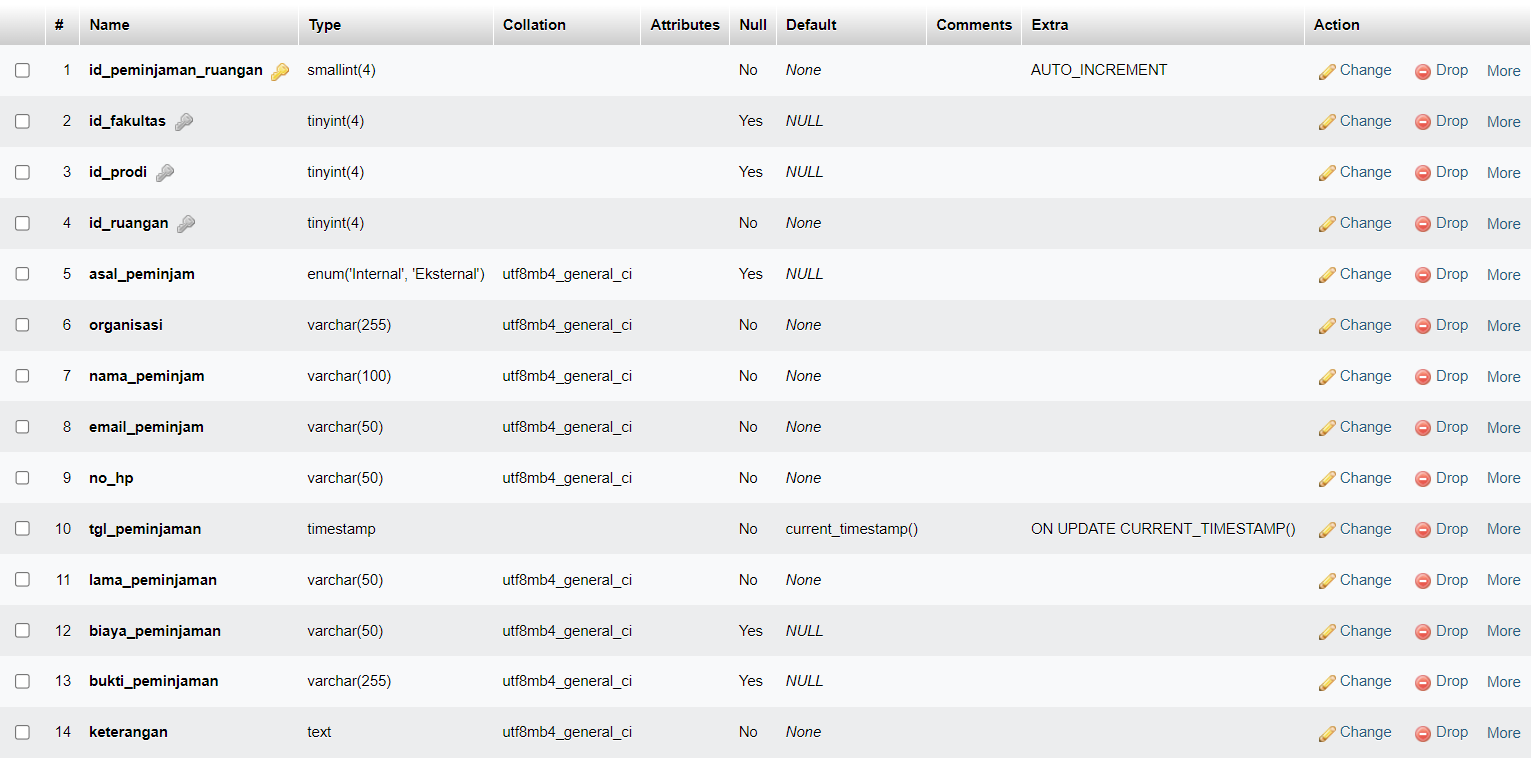
\includegraphics[width=0.82\linewidth]{konten//gambar/Tampilan database tabel peminjaman_ruangan.png}
          \caption{Tampilan \textit{Database} Tabel peminjaman\_ruangan}
          \label{fig:enter-label}
        \end{figure}

  \item Struktur Tabel Pemusnahan Barang
        Pada tabel data pemusnahan\_barang terdiri dari kolom
        id\_musnah yang menjadi kunci utama dari tabel tersebut yang digunakan sebagai penanda agar tidak terjadi duplikasi data, id\_barang menjadi kunci asing dalam tabel pemusnahan barang karena nama barang diperlukan dalam pencatatan data pemusnahan barang, tgl\_pemusnahan merupakan kolom untuk menyimpan tanggal dilakukannya pemusnahan barang, bukti\_pemusnahan merupakan kolom untuk menyimpan dokumen bukti pemusnahan, waktu untuk mendeteksi kapan waktu dimusnahkannya barang, alasan merupakan kolom untuk menyimpan alasan dilakukannya pemusnahan barang. Tampilan dapat dilihat pada Gambar 4.9.

        \begin{figure}
          \centering
          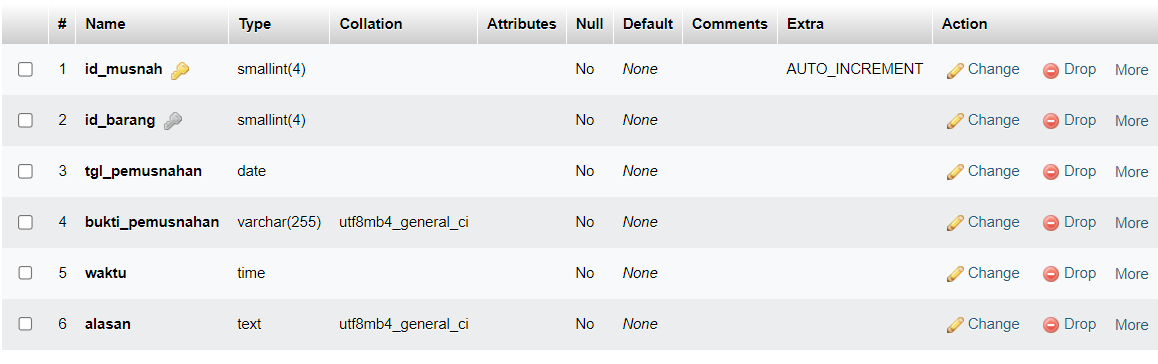
\includegraphics[width=0.82\linewidth]{konten//gambar/Tampilan database tabel pemusnahan_barang.png}
          \caption{Tampilan \textit{Database} Tabel pemusnahan\_barang}
          \label{fig:enter-label}
        \end{figure}

  \item Struktur Tabel Pendanaan
        Pada tabel data pendanaan terdiri dari kolom id\_pendanaan yang menjadi kunci utama dari tabel tersebut yang digunakan sebagai penanda agar tidak terjadi duplikasi data, jenis\_pendanaan merupakan kolom untuk menyimpan apa jenis pendanaannya, keterangan merupakan kolom untuk menyimpan data keterangan dari pendanaan. Tampilan dapat dilihat pada Gambar 4.10.

        \begin{figure}
          \centering
          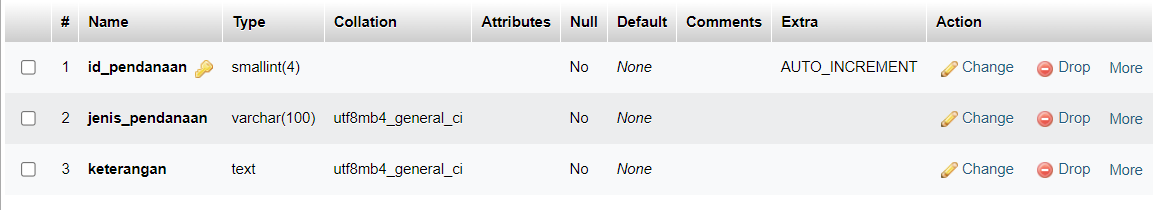
\includegraphics[width=0.82\linewidth]{konten//gambar/Tampilan database tabel pendanaan.png}
          \caption{Tampilan \textit{Database} Tabel pendanaan}
          \label{fig:enter-label}
        \end{figure}

  \item Struktur Tabel Prodi
        Pada tabel data prodi terdiri dari kolom id\_prodi yang menjadi kunci utama dari tabel tersebut yang digunakan sebagai penanda agar tidak terjadi duplikasi data, id\_fakultas menjadi kunci asing dalam tabel prodi karena nama fakultas diperlukan dalam pencatatan data prodi, nama\_prodi merupakan kolom untuk mencatat nama prodi. Tampilan dapat dilihat pada Gambar 4.11.

        \begin{figure}
          \centering
          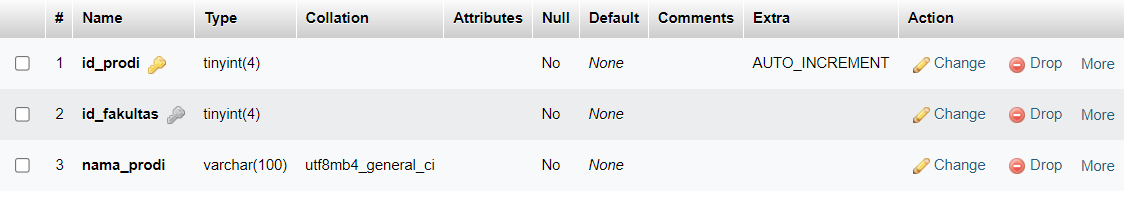
\includegraphics[width=0.82\linewidth]{konten//gambar/Tampilan database tabel prodi.png}
          \caption{Tampilan \textit{Database} Tabel prodi}
          \label{fig:enter-label}
        \end{figure}

  \item Struktur Tabel Referensi
        Pada tabel data referensi terdiri dari kolom id\_referensi yang menjadi kunci utama dari tabel tersebut yang digunakan sebagai penanda agar tidak terjadi duplikasi data, biaya kolom untuk menampilkan biaya peminjaman pada peminjam eksternal yang digunakan pada tabel peminjaman barang dan peminjaman ruangan. Tampilan dapat dilihat pada Gambar 4.12.

        \begin{figure}
          \centering
          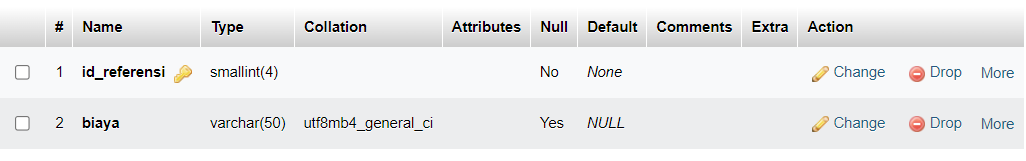
\includegraphics[width=0.82\linewidth]{konten//gambar/Tampilan database tabel referensi.png}
          \caption{Tampilan \textit{Database} Tabel referensi}
          \label{fig:enter-label}
        \end{figure}

  \item Struktur Tabel Ruangan
        Pada tabel data ruangan terdiri dari kolom id\_ruangan yang menjadi kunci utama dari tabel tersebut yang digunakan sebagai penanda agar tidak terjadi duplikasi data, id\_gedung menjadi kunci asing dalam tabel ruangan karena nama gedung diperlukan dalam pencatatan data ruangan, nama\_ruangan adalah kolom yang menyimpan nama ruangan yang dicatat, deskripsi\_ruangan menjelaskan detail tentang ruangan yang dicatat, gambar\_ruangan merupakan kolom untuk menyimpan data gambar dari ruangan yang dicatat. Tampilan dapat dilihat pada Gambar 4.13.

        \begin{figure}
          \centering
          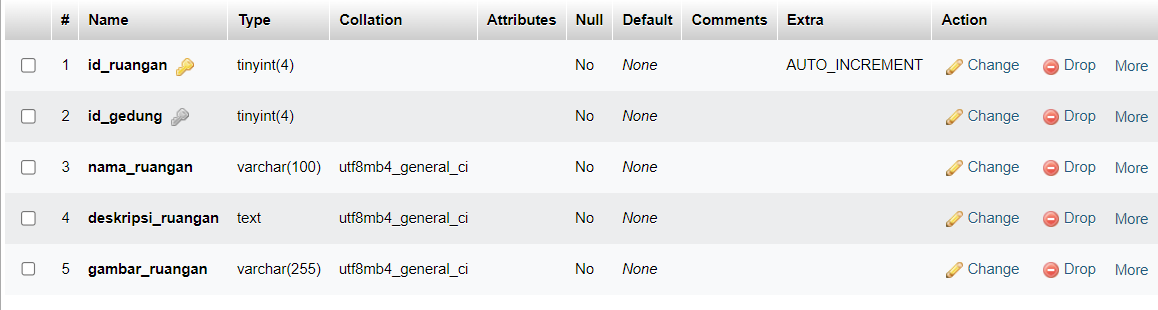
\includegraphics[width=0.82\linewidth]{konten//gambar/Tampilan database tabel ruangan.png}
          \caption{Tampilan \textit{Database} Tabel ruangan}
          \label{fig:enter-label}
        \end{figure}

  \item Struktur Tabel User
        Pada tabel data user terdiri dari kolom id\_user yang menjadi kunci utama dari tabel tersebut yang digunakan sebagai penanda agar tidak terjadi duplikasi data, nama merupakan kolom yang menyimpan nama pengguna, foto merupakan kolom untuk menyimpan foto profil pengguna, no\_identitas merupakan kolom yang digunakan untuk menyimpan data NIM, NIP, atau NIK dari pengguna, \textit{username} merupakan kolom yang digunakan untuk menyimpan \textit{username} pengguna, password\_hash merupakan kolom yang digunakan untuk menyimpan \textit{password} pengguna, email merupakan kolom yang digunakan untuk menyimpan email pengguna, role\_user merupakan kolom yang digunakan untuk menyimpan level akses pengguna. Tampilan dapat dilihat pada Gambar 4.14.

        \begin{figure}
          \centering
          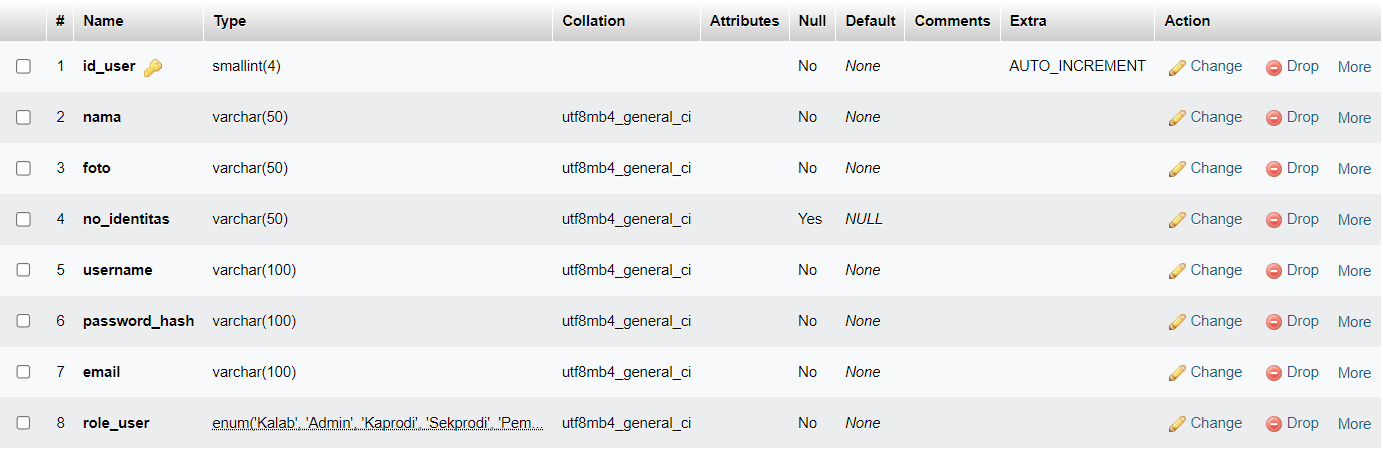
\includegraphics[width=0.82\linewidth]{konten//gambar/Tampilan database tabel user.png}
          \caption{Tampilan \textit{Database} Tabel user}
          \label{fig:enter-label}
        \end{figure}

\end{enumerate}

% -----------------------------------------------------------------------------%
\section{Implementasi Kode Pemrograman}
\subsection{\textit{Routes}}
\textit{Routes} dalam konsep MVC \textit{(Model-View-Controller)} adalah mekanisme yang digunakan untuk mengatur bagaimana permintaan (\textit{requests}) dari pengguna atau klien akan ditangani oleh aplikasi web. \textit{Routes} menentukan hubungan antara URL yang diminta oleh pengguna dengan \textit{controller} yang akan menangani permintaan tersebut \cite{kelvin2022sistem}.

\begin{enumerate}
  \item \textit{Routes} dalam implementasi sistem informasi inventaris laboratorium pada data barang dapat dilihat pada Gambar 4.15.

        \begin{figure}
          \centering
          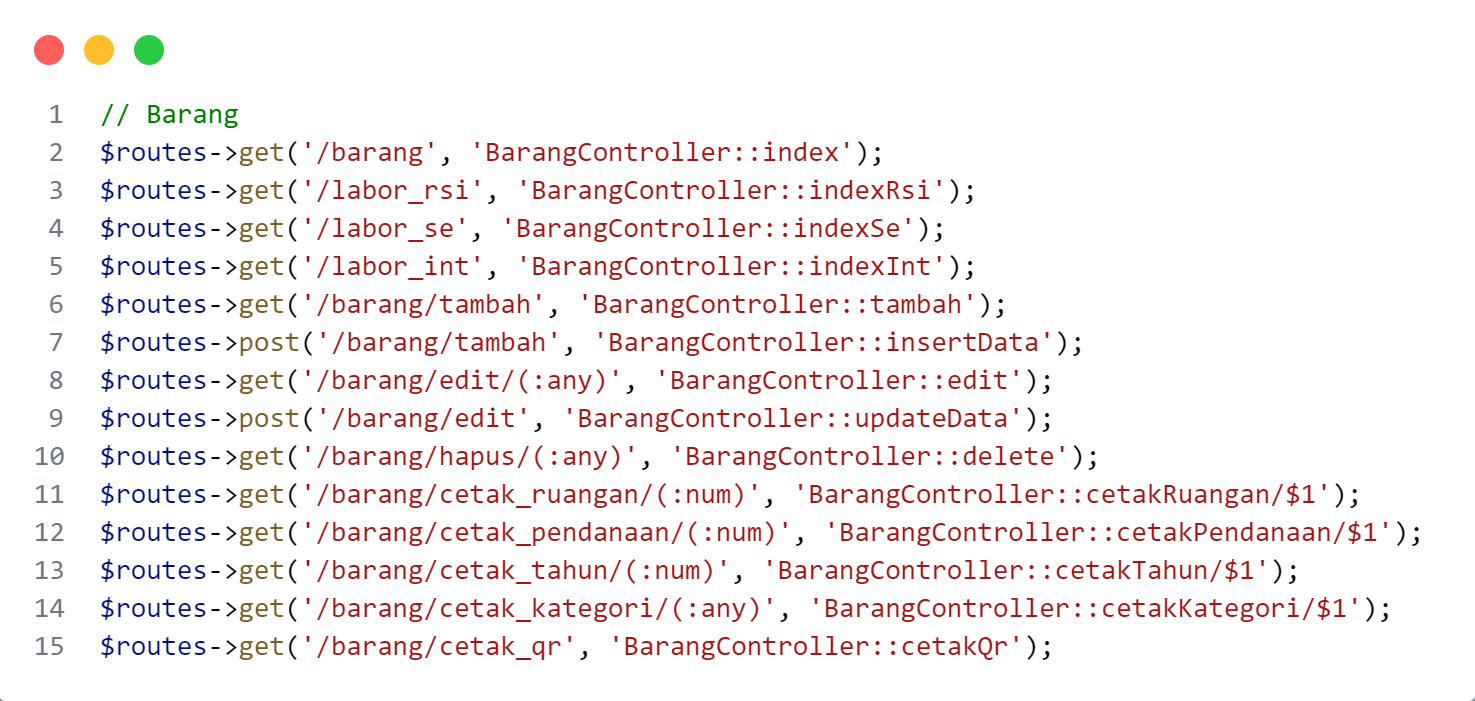
\includegraphics[width=0.82\linewidth]{konten//gambar/routes barang.png}
          \caption{\textit{Routes} Barang}
          \label{fig:enter-label}
        \end{figure}

  \item \textit{Routes} dalam implementasi sistem informasi inventaris laboratorium pada data dokumentasi dapat dilihat pada Gambar 4.16.

        \begin{figure}
          \centering
          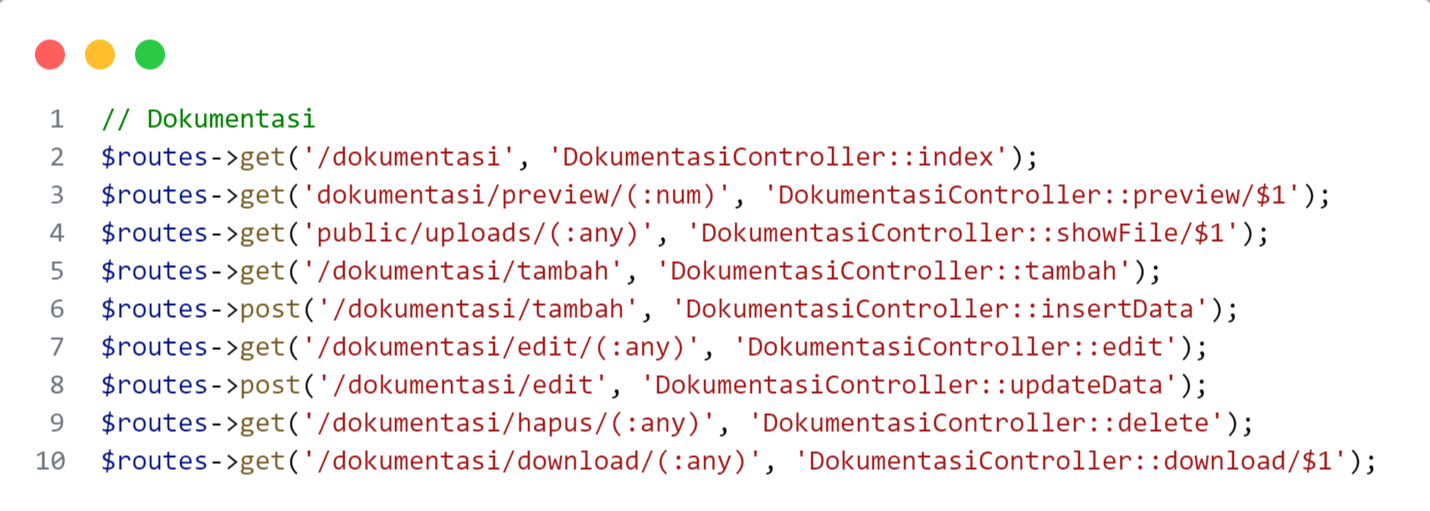
\includegraphics[width=0.82\linewidth]{konten//gambar/routes dokumentasi.png}
          \caption{\textit{Routes} Dokumentasi}
          \label{fig:enter-label}
        \end{figure}

  \item \textit{Routes} dalam implementasi sistem informasi inventaris laboratorium pada data fakultas dapat dilihat pada Gambar 4.17.

        \begin{figure}
          \centering
          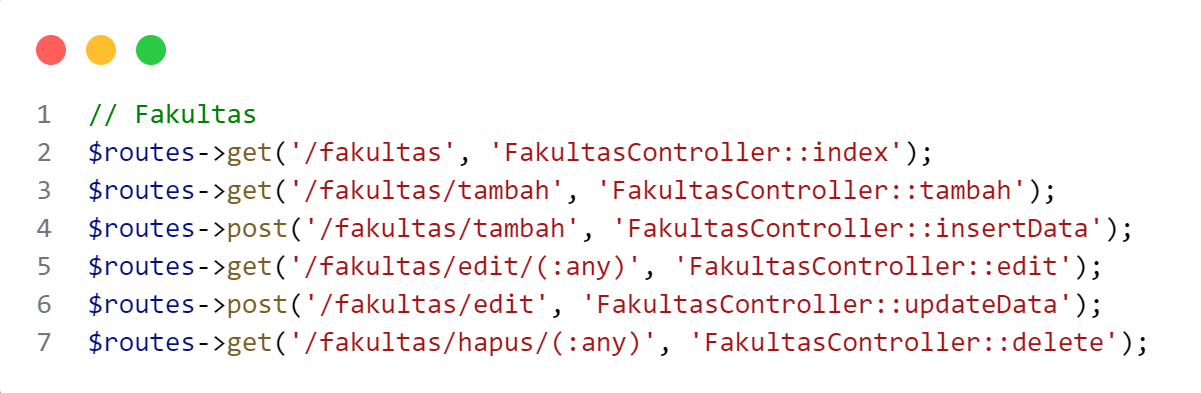
\includegraphics[width=0.82\linewidth]{konten//gambar/routes fakultas.png}
          \caption{\textit{Routes} Fakultas}
          \label{fig:enter-label}
        \end{figure}

  \item \textit{Routes} dalam implementasi sistem informasi inventaris laboratorium pada data gedung dapat dilihat pada Gambar 4.18.

        \begin{figure}
          \centering
          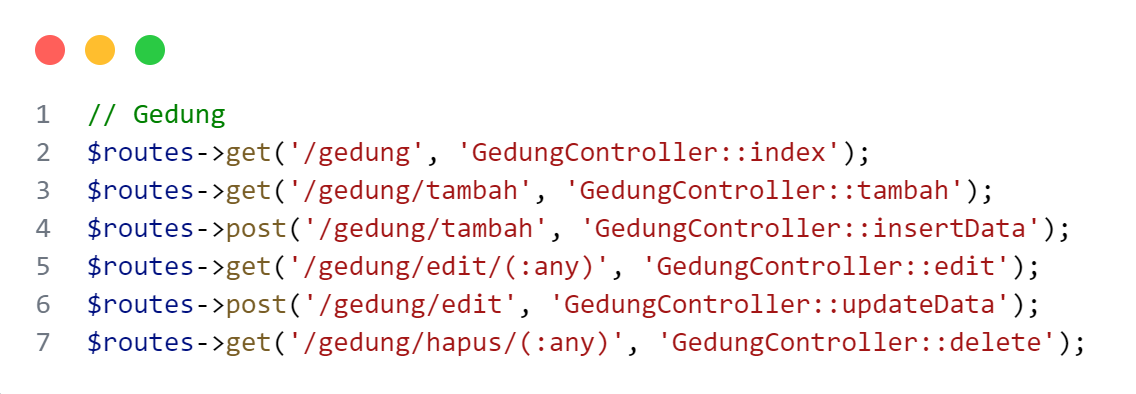
\includegraphics[width=0.82\linewidth]{konten//gambar/routes gedung.png}
          \caption{\textit{Routes} Gedung}
          \label{fig:enter-label}
        \end{figure}

  \item \textit{Routes} dalam implementasi sistem informasi inventaris laboratorium pada data \textit{maintenance} dapat dilihat pada Gambar 4.19.

        \begin{figure}
          \centering
          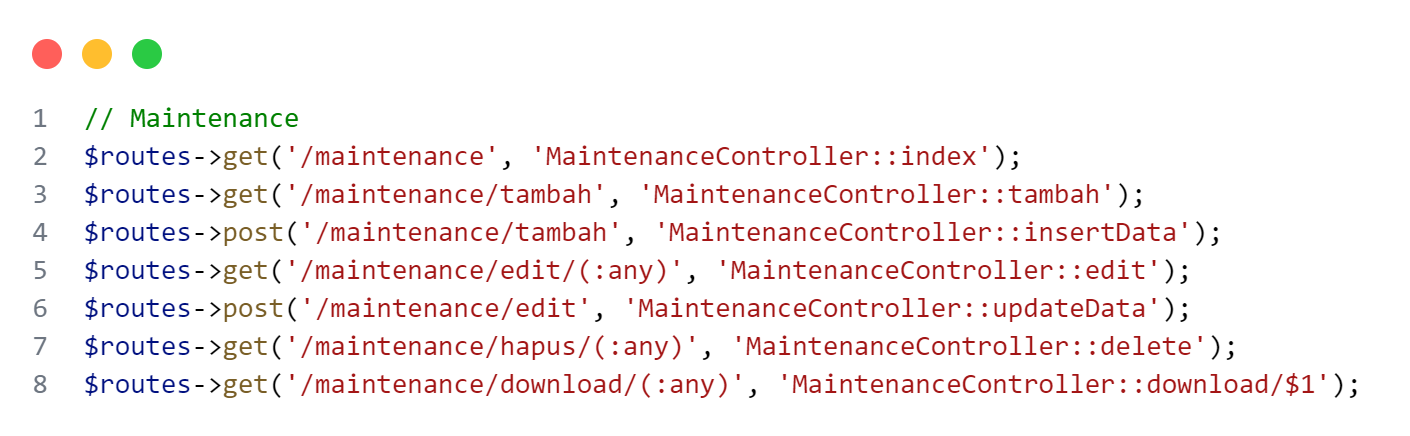
\includegraphics[width=0.82\linewidth]{konten//gambar/routes maintenance.png}
          \caption{\textit{Routes Maintenance}}
          \label{fig:enter-label}
        \end{figure}

  \item \textit{Routes} dalam implementasi sistem informasi inventaris laboratorium pada data peminjaman barang dapat dilihat pada Gambar 4.20.

        \begin{figure}
          \centering
          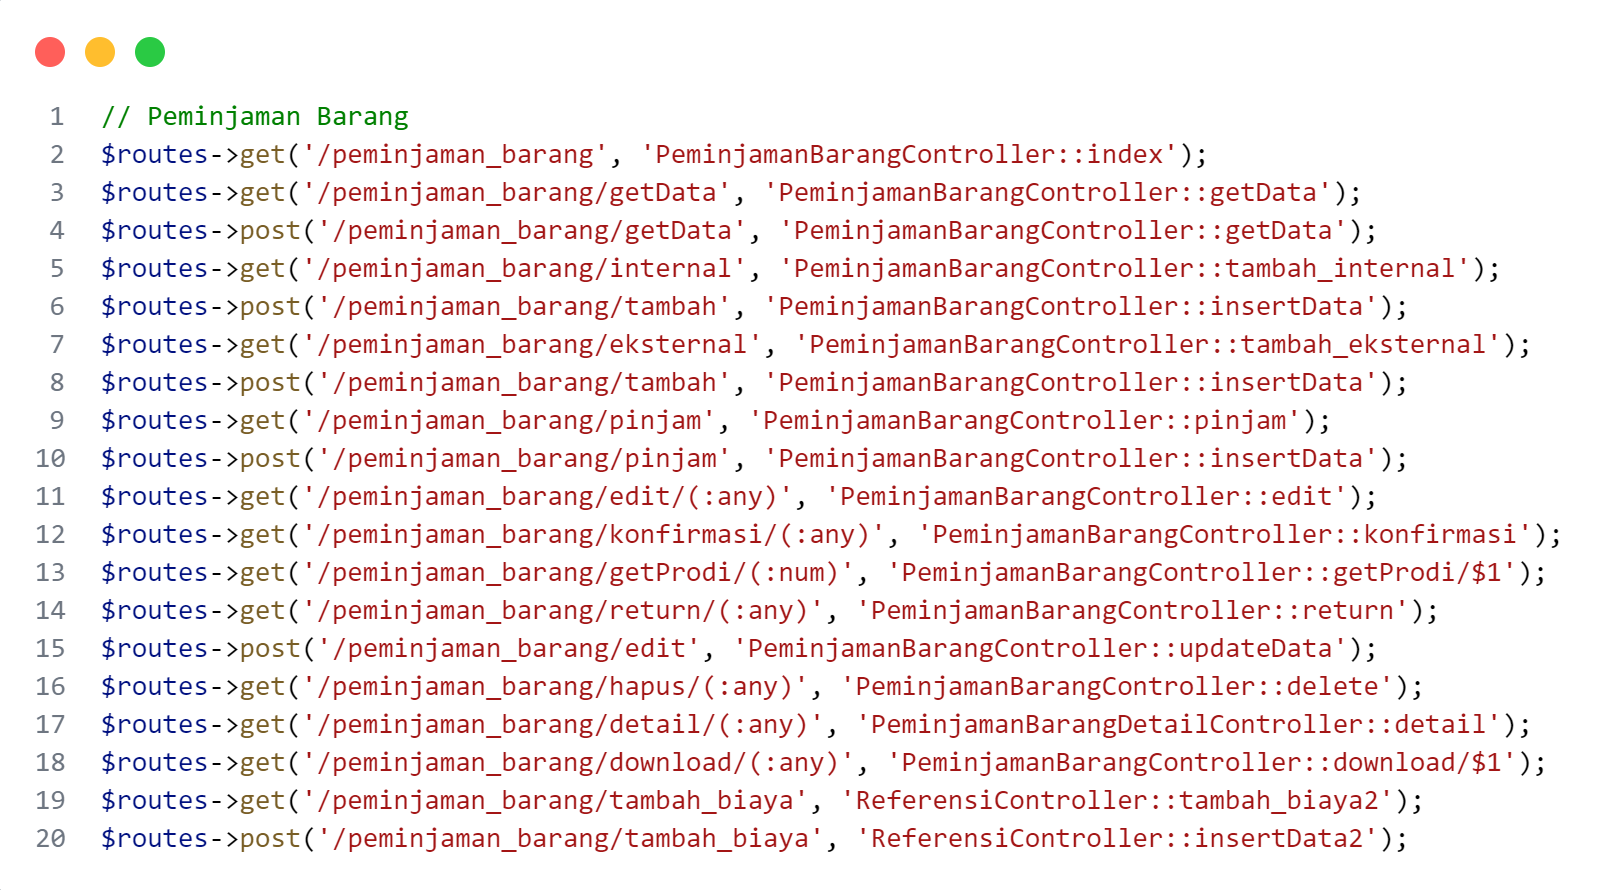
\includegraphics[width=0.82\linewidth]{konten//gambar/routes peminjaman barang.png}
          \caption{\textit{Routes} Peminjaman Barang}
          \label{fig:enter-label}
        \end{figure}

  \item \textit{Routes} dalam implementasi sistem informasi inventaris laboratorium pada data peminjaman ruangan dapat dilihat pada Gambar 4.21.

        \begin{figure}
          \centering
          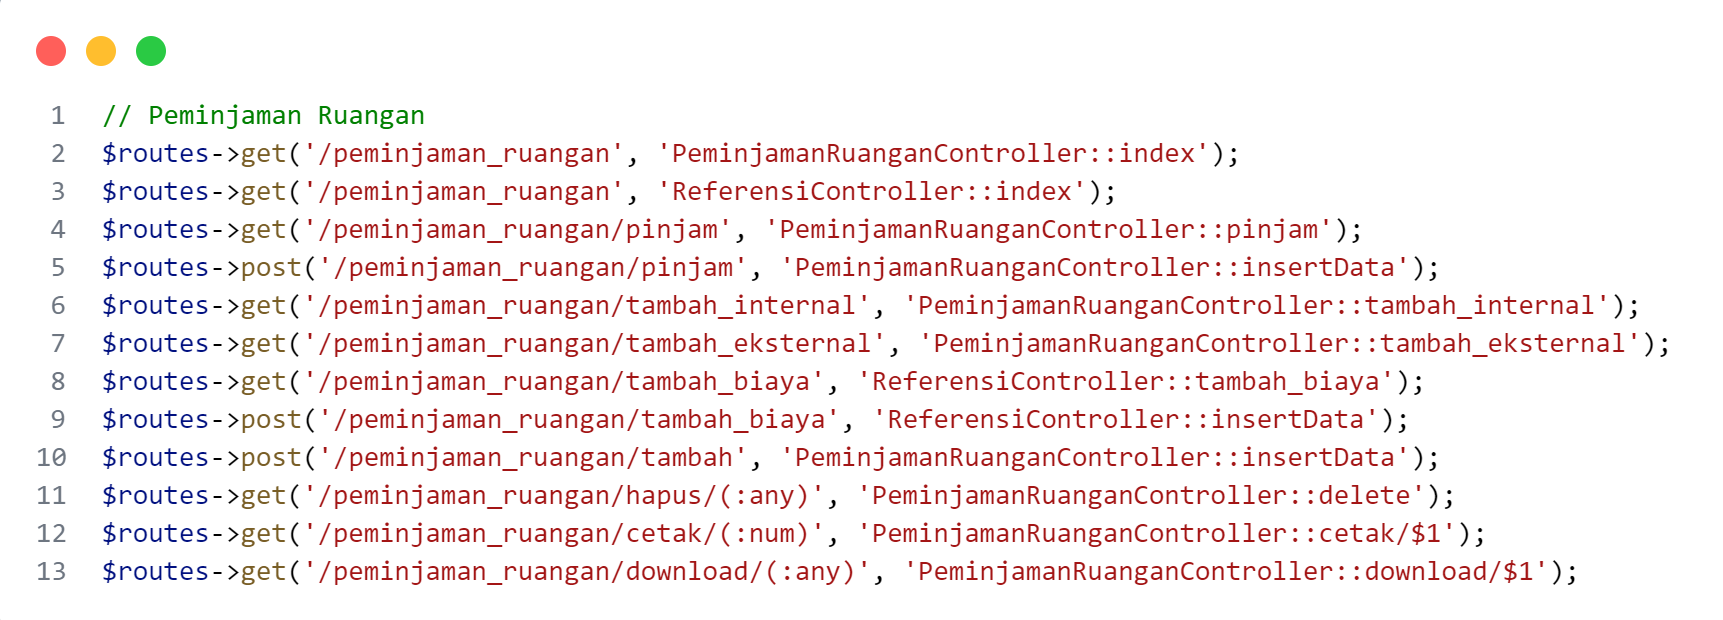
\includegraphics[width=0.82\linewidth]{konten//gambar/routes peminjaman ruangan.png}
          \caption{\textit{Routes} Peminjaman Ruangan}
          \label{fig:enter-label}
        \end{figure}

  \item \textit{Routes} dalam implementasi sistem informasi inventaris laboratorium pada data pemusnahan barang dapat dilihat pada Gambar 4.22.

        \begin{figure}
          \centering
          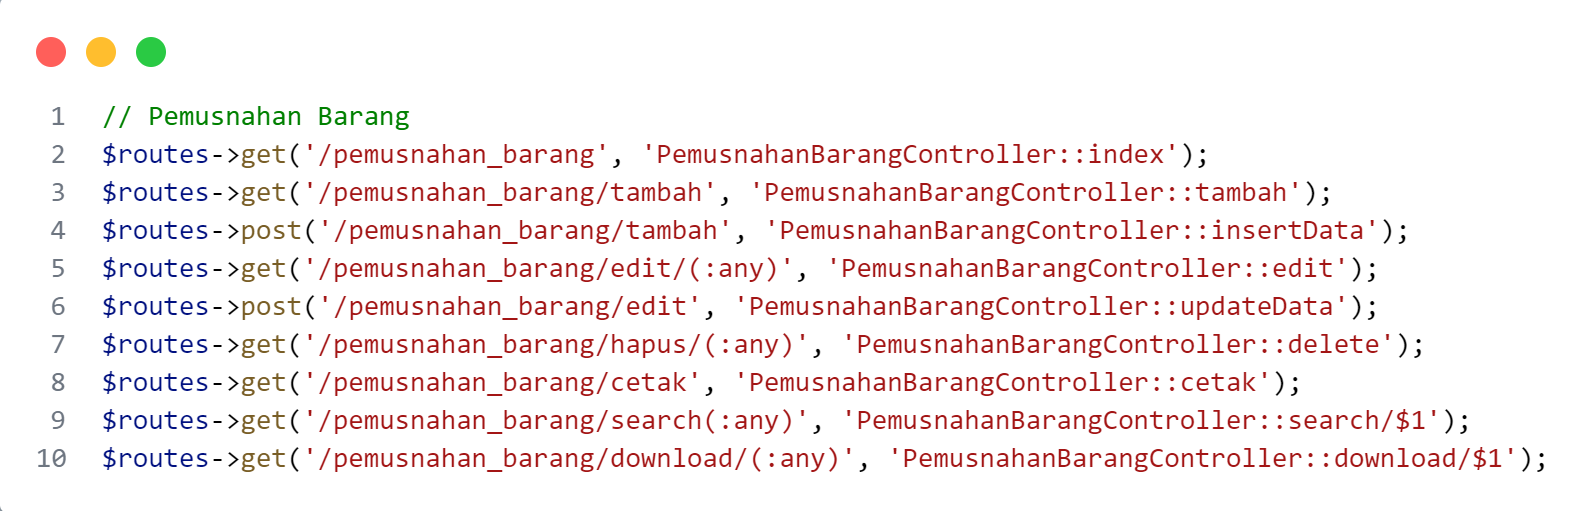
\includegraphics[width=0.82\linewidth]{konten//gambar/routes pemusnahan barang.png}
          \caption{\textit{Routes} Pemusnahan Barang}
          \label{fig:enter-label}
        \end{figure}

  \item \textit{Routes} dalam implementasi sistem informasi inventaris laboratorium pada data pendanaan dapat dilihat pada Gambar 4.23.

        \begin{figure}
          \centering
          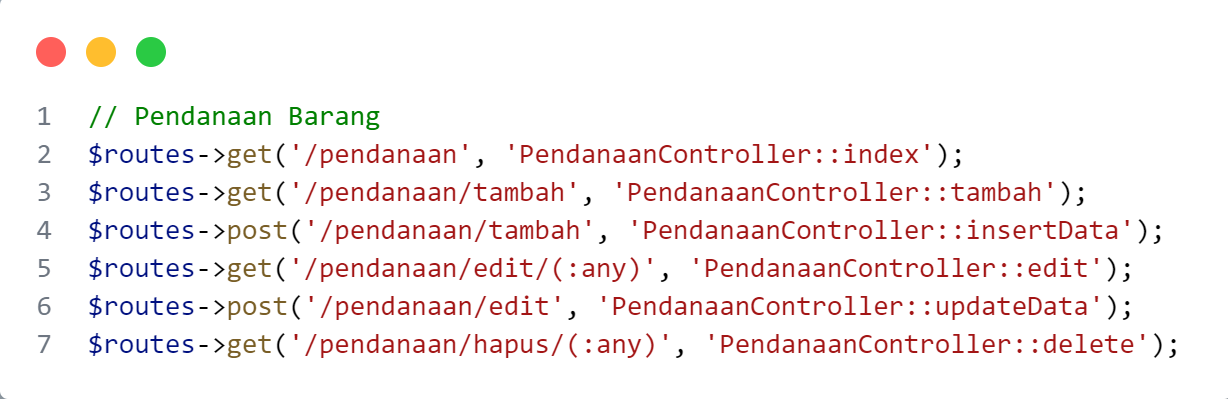
\includegraphics[width=0.82\linewidth]{konten//gambar/routes pendanaan.png}
          \caption{\textit{Routes} Pendanaan}
          \label{fig:enter-label}
        \end{figure}

  \item \textit{Routes} dalam implementasi sistem informasi inventaris laboratorium pada data prodi dapat dilihat pada Gambar 4.24.

        \begin{figure}
          \centering
          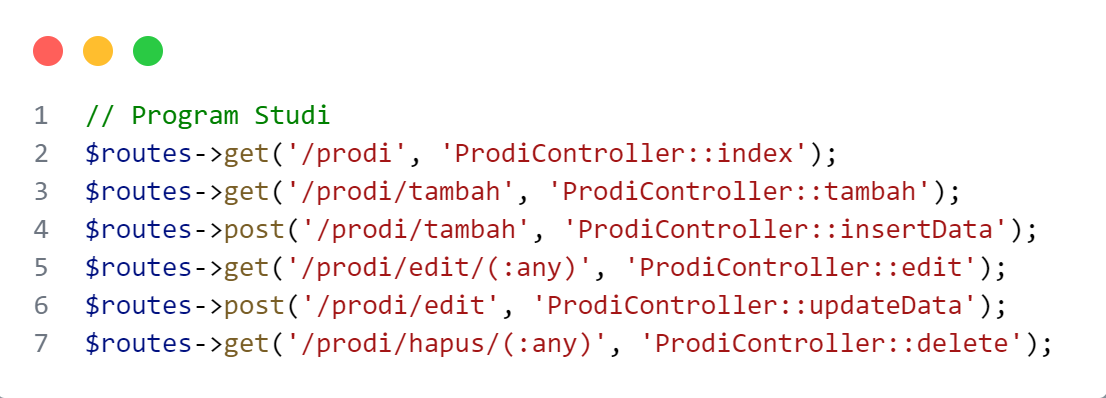
\includegraphics[width=0.82\linewidth]{konten//gambar/routes prodi.png}
          \caption{\textit{Routes} Prodi}
          \label{fig:enter-label}
        \end{figure}

  \item \textit{Routes} dalam implementasi sistem informasi inventaris laboratorium pada data ruangan dapat dilihat pada Gambar 4.25.

        \begin{figure}
          \centering
          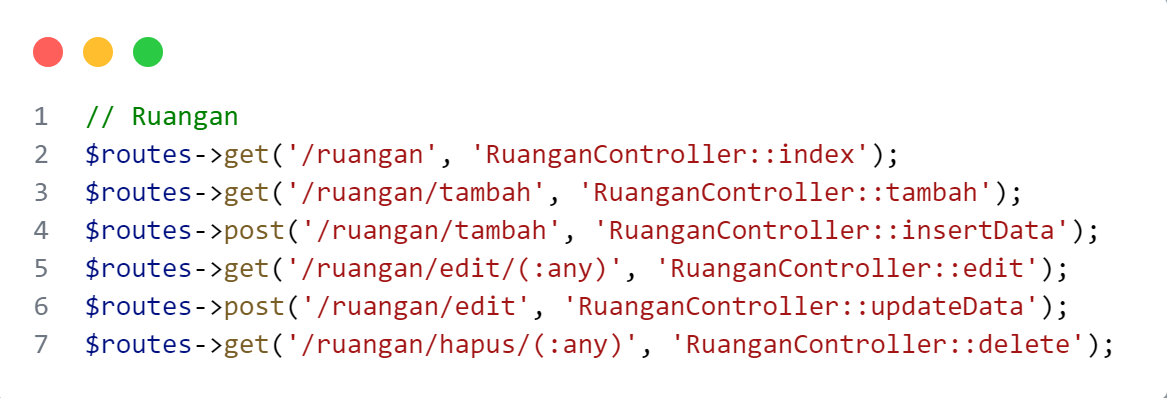
\includegraphics[width=0.82\linewidth]{konten//gambar/routes ruangan.png}
          \caption{\textit{Routes} Ruangan}
          \label{fig:enter-label}
        \end{figure}

  \item \textit{Routes} dalam implementasi sistem informasi inventaris laboratorium pada data \textit{user} dapat dilihat pada Gambar 4.26.

        \begin{figure}
          \centering
          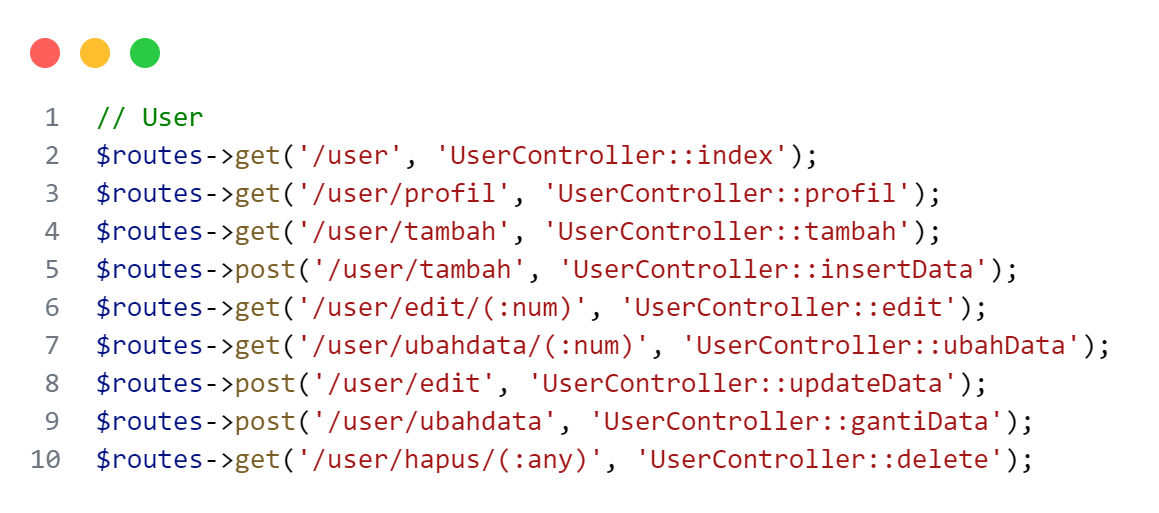
\includegraphics[width=0.82\linewidth]{konten//gambar/routes user.png}
          \caption{\textit{Routes} \textit{User}}
          \label{fig:enter-label}
        \end{figure}
\end{enumerate}

\subsection{Model}
Model adalah komponen yang bertanggung jawab untuk mengatur data, aturan bisnis, dan logika aplikasi. Ini merupakan representasi dari data dalam aplikasi. Model mengelola semua operasi data, seperti pengambilan, pembaruan, dan penyimpanan data \cite{firdaus2020rancang}.

\begin{enumerate}
  \item Model dalam implementasi sistem informasi inventaris laboratorium pada data barang dapat dilihat pada Gambar 4.27.

        \begin{figure}
          \centering
          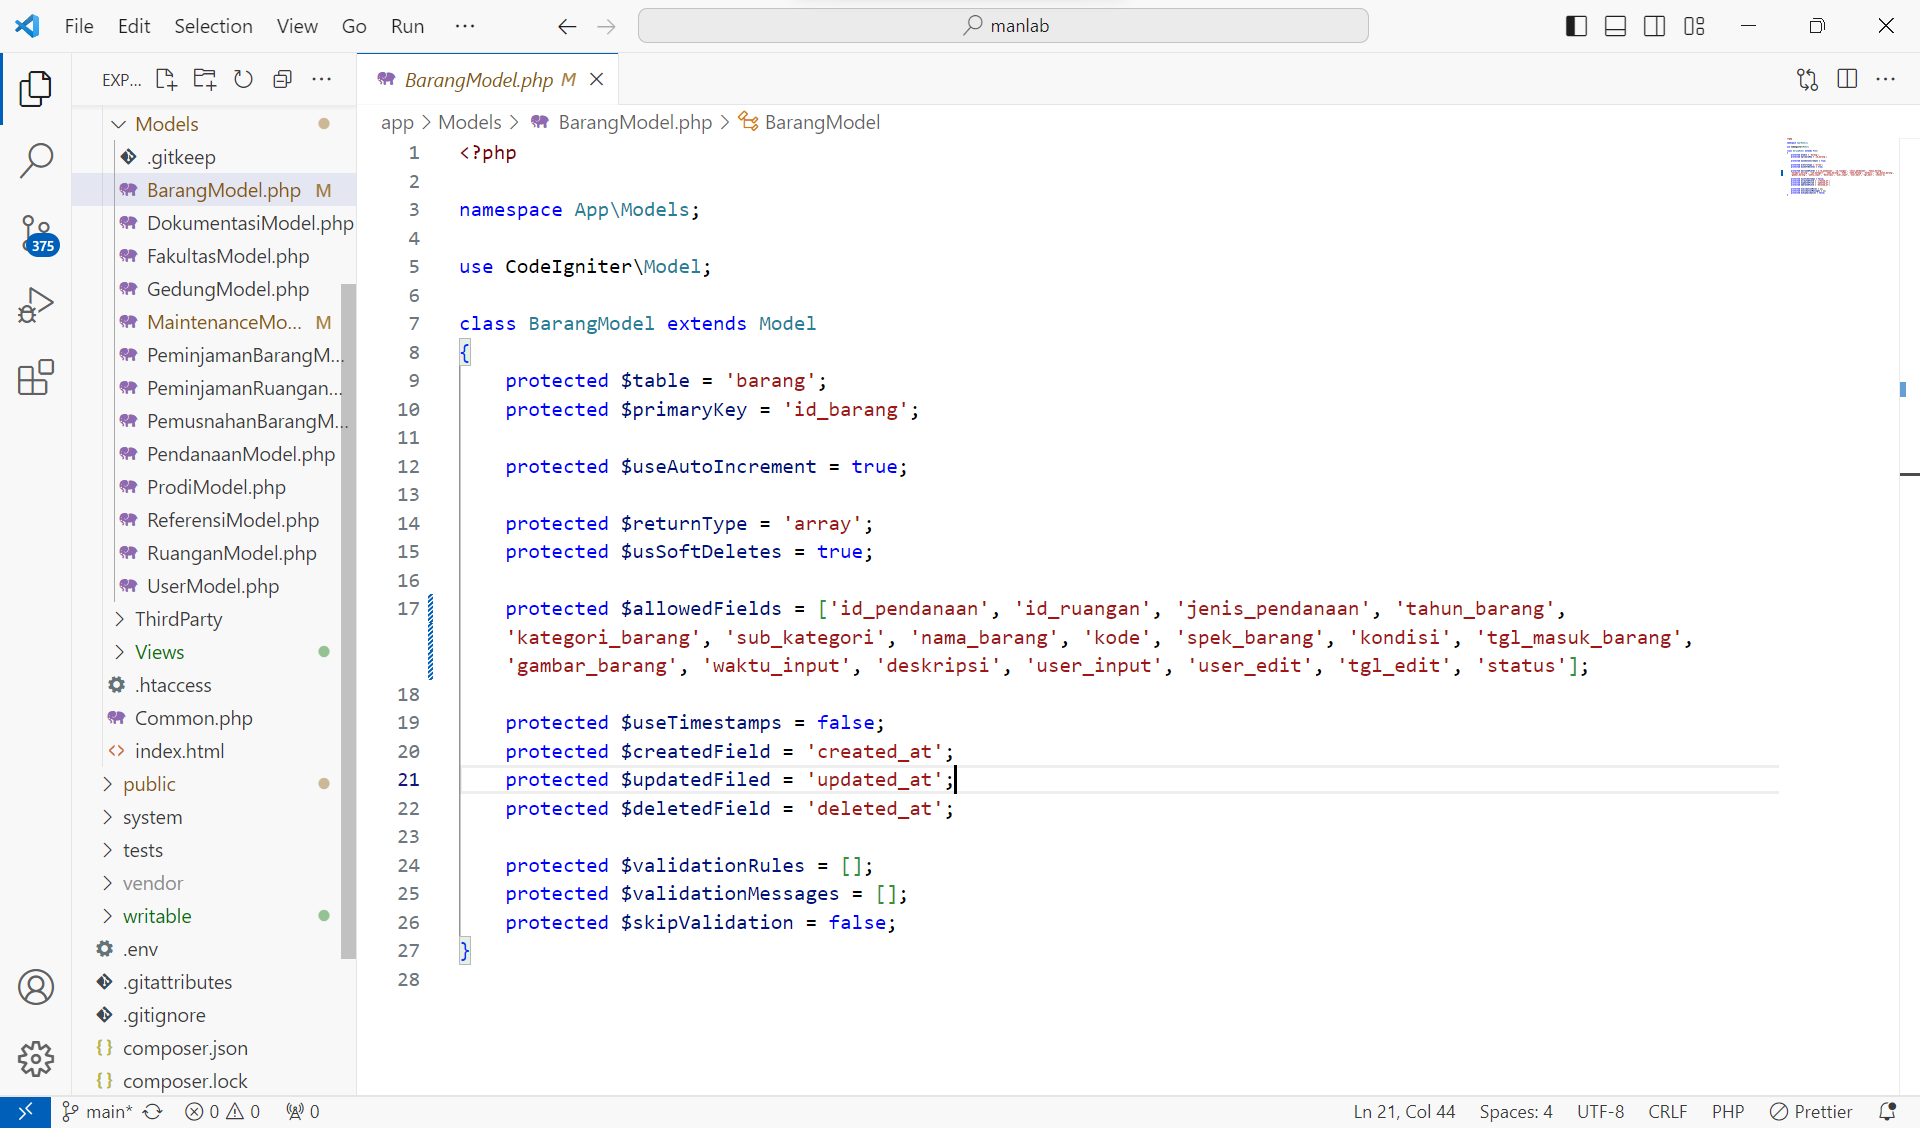
\includegraphics[width=0.82\linewidth]{konten//gambar/barang model.png}
          \caption{Model Barang}
          \label{fig:enter-label}
        \end{figure}

  \item Model dalam implementasi sistem informasi inventaris laboratorium pada data dokumentasi dapat dilihat pada Gambar 4.28.

        \begin{figure}
          \centering
          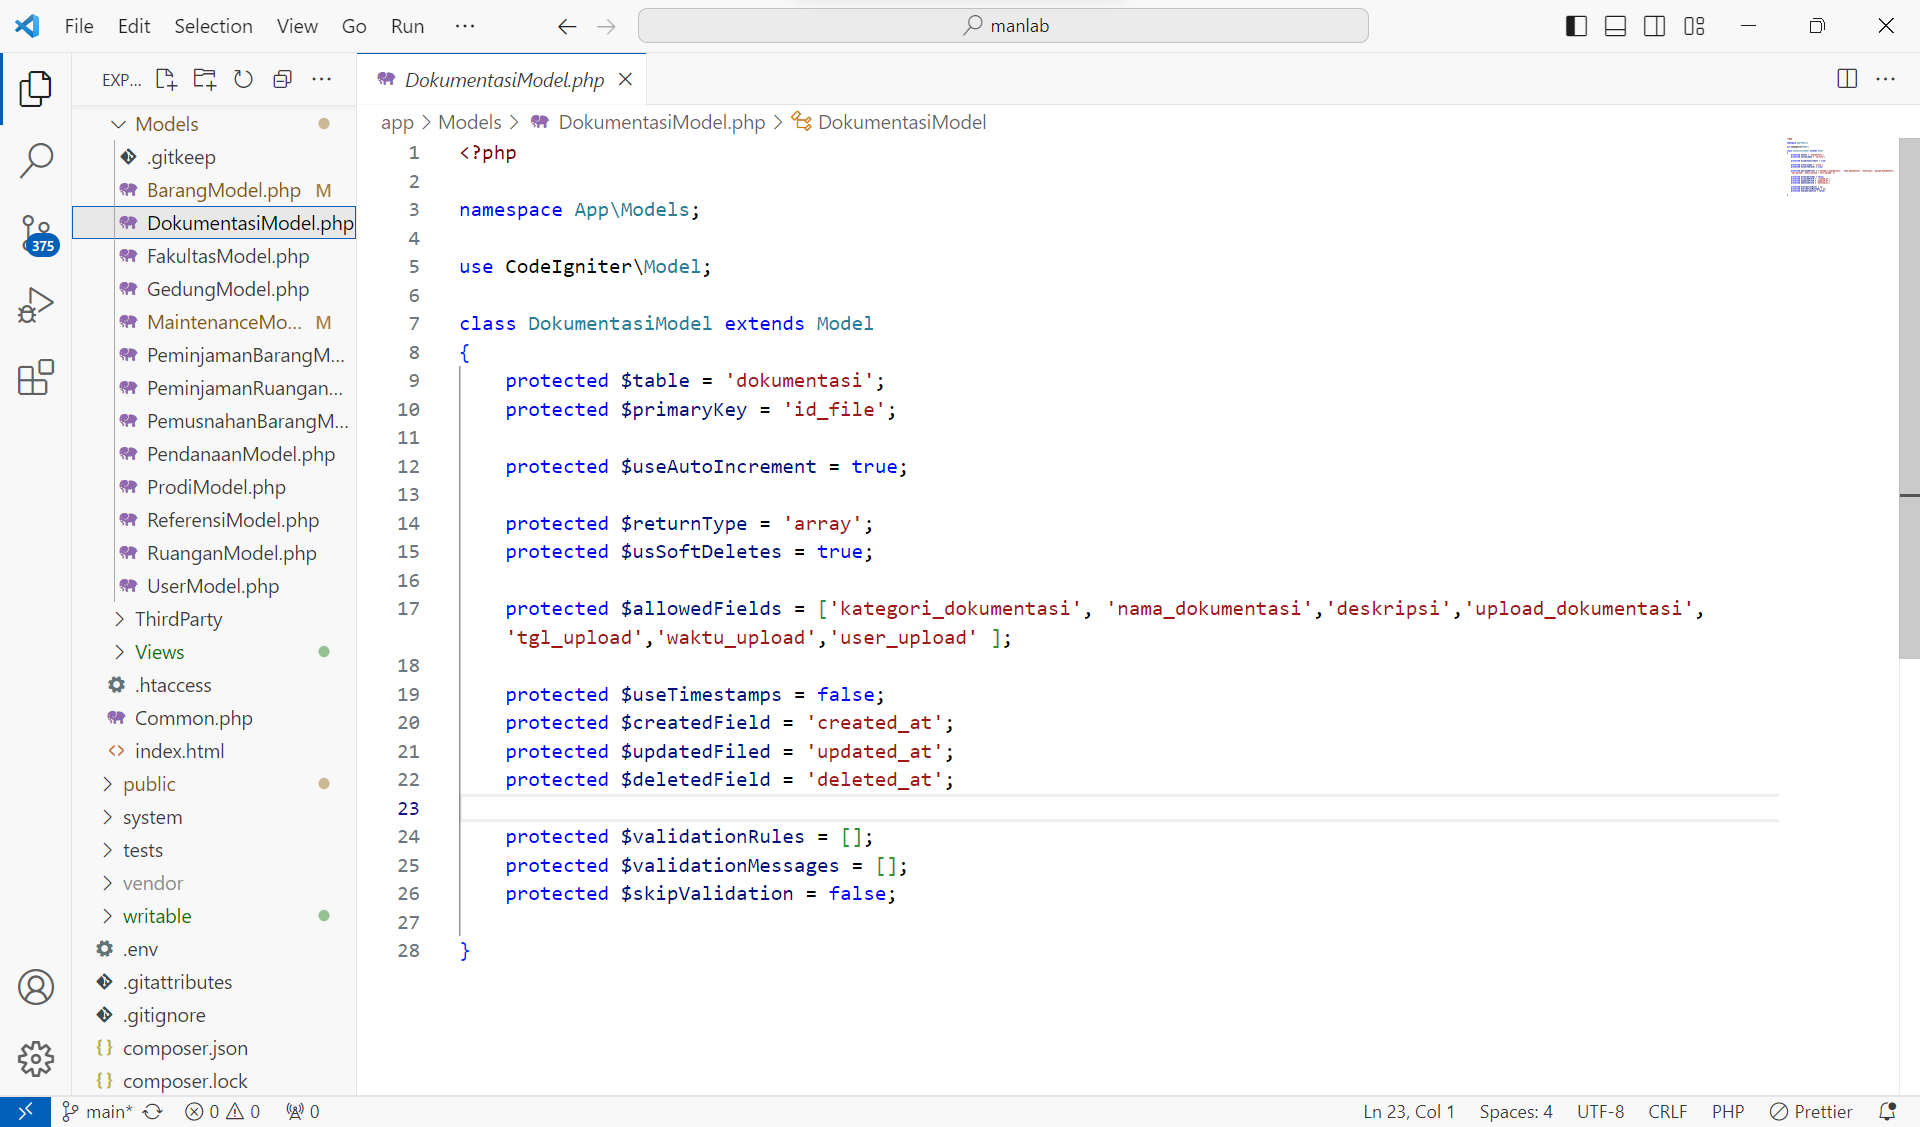
\includegraphics[width=0.82\linewidth]{konten//gambar/dokumentasi model.png}
          \caption{Model Dokumentasi}
          \label{fig:enter-label}
        \end{figure}

  \item Model dalam implementasi sistem informasi inventaris laboratorium pada data fakultas dapat dilihat pada Gambar 4.29.

        \begin{figure}
          \centering
          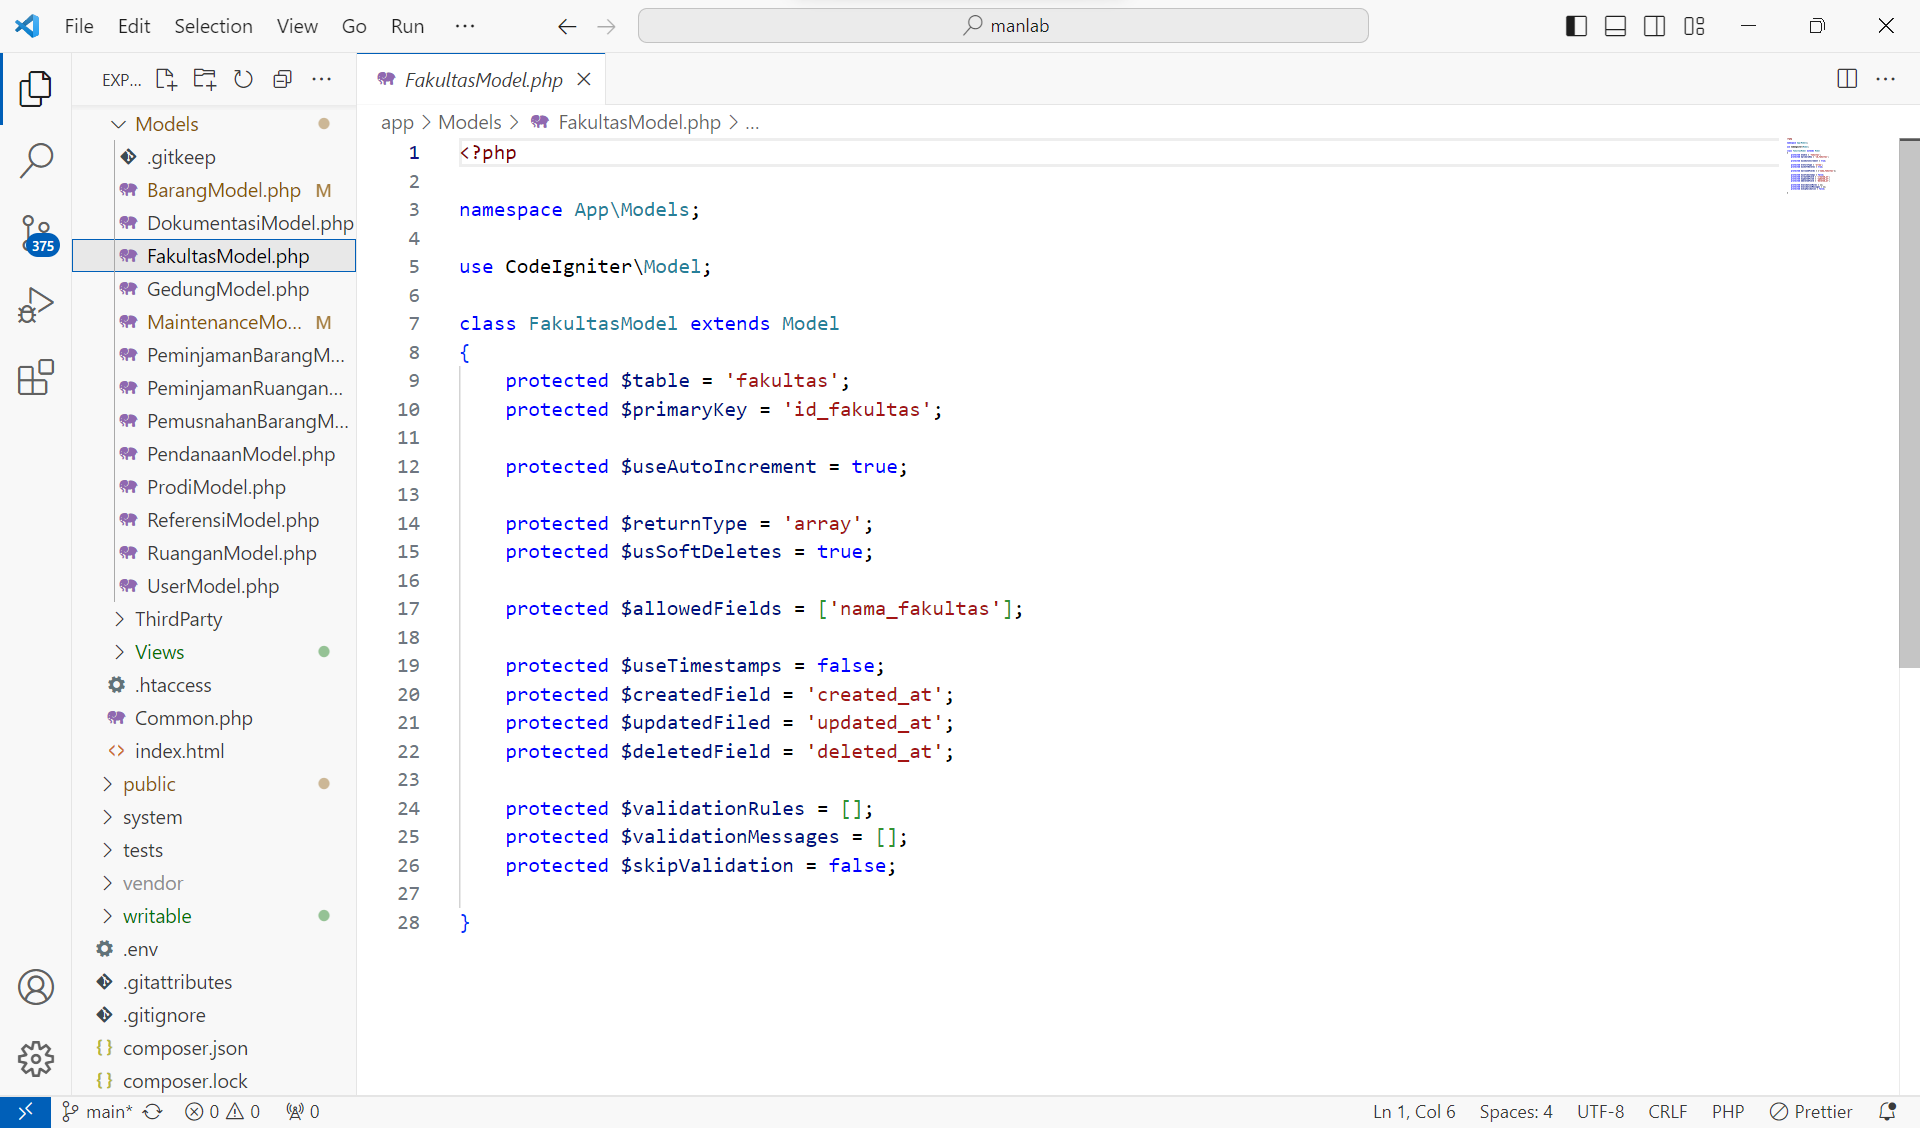
\includegraphics[width=0.82\linewidth]{konten//gambar/fakultas model.png}
          \caption{Model Fakultas}
          \label{fig:enter-label}
        \end{figure}

  \item Model dalam implementasi sistem informasi inventaris laboratorium pada data gedung dapat dilihat pada Gambar 4.30.

        \begin{figure}
          \centering
          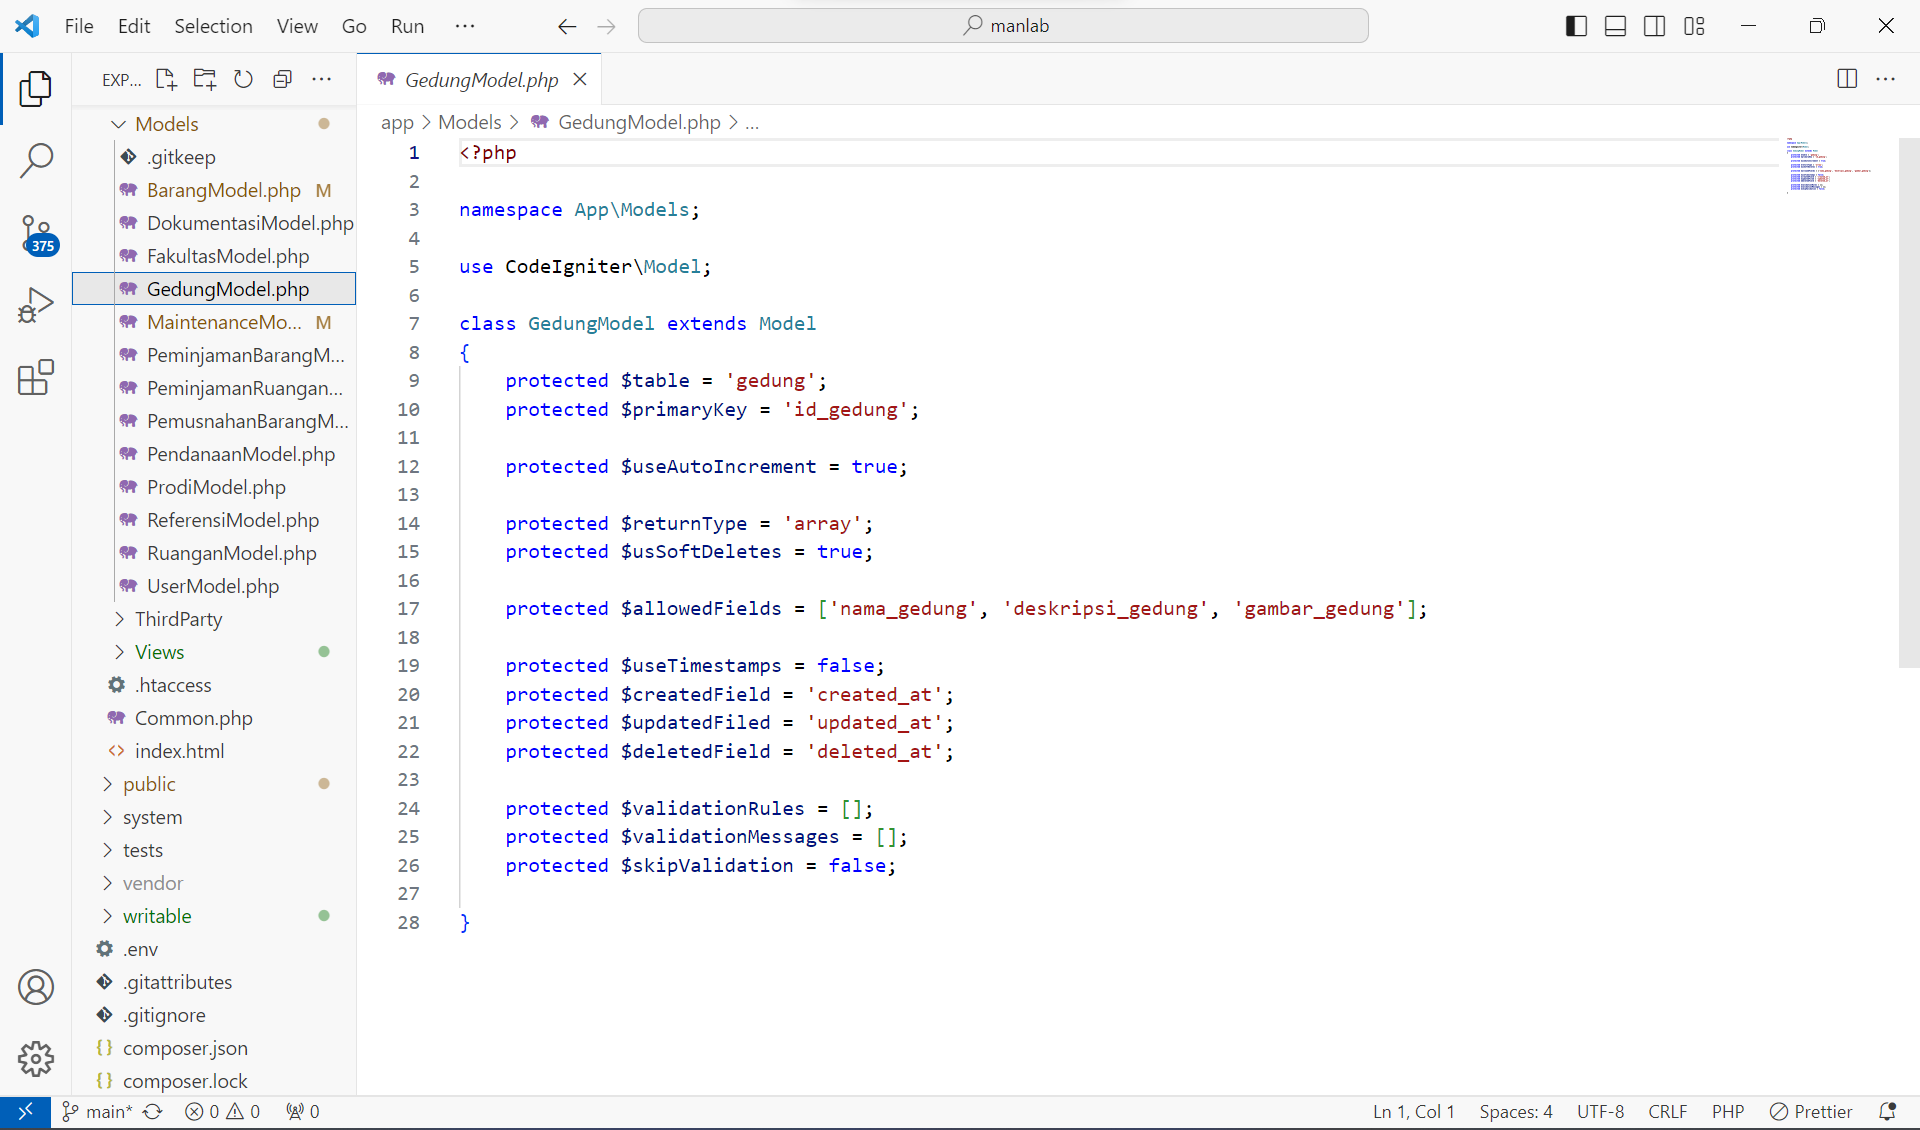
\includegraphics[width=0.82\linewidth]{konten//gambar/gedung model.png}
          \caption{Model Gedung}
          \label{fig:enter-label}
        \end{figure}

  \item Model dalam implementasi sistem informasi inventaris laboratorium pada data \textit{maintenance} dapat dilihat pada Gambar 4.31.

        \begin{figure}
          \centering
          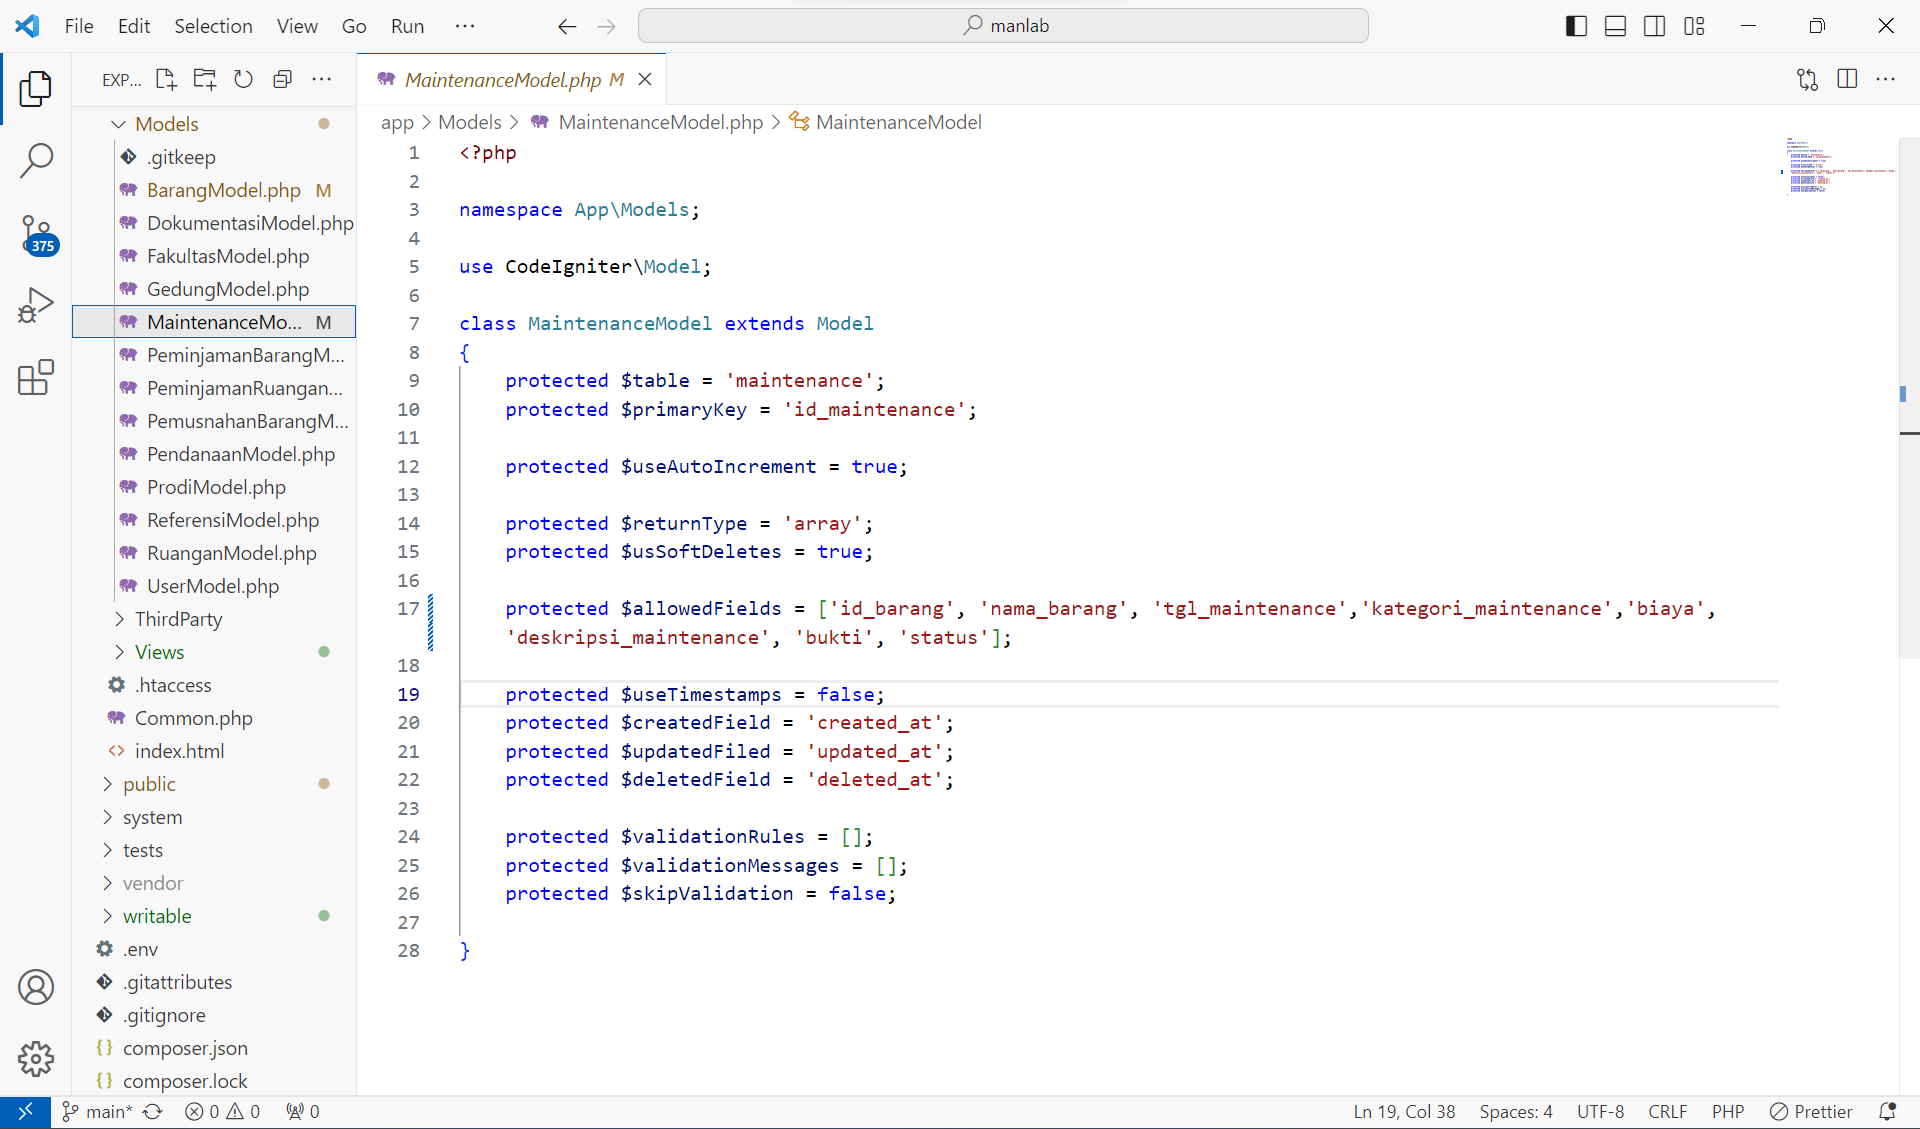
\includegraphics[width=0.82\linewidth]{konten//gambar/maintenance model.png}
          \caption{Model \textit{Maintenance}}
          \label{fig:enter-label}
        \end{figure}

  \item Model dalam implementasi sistem informasi inventaris laboratorium pada data peminjaman barang dapat dilihat pada Gambar 4.32.

        \begin{figure}
          \centering
          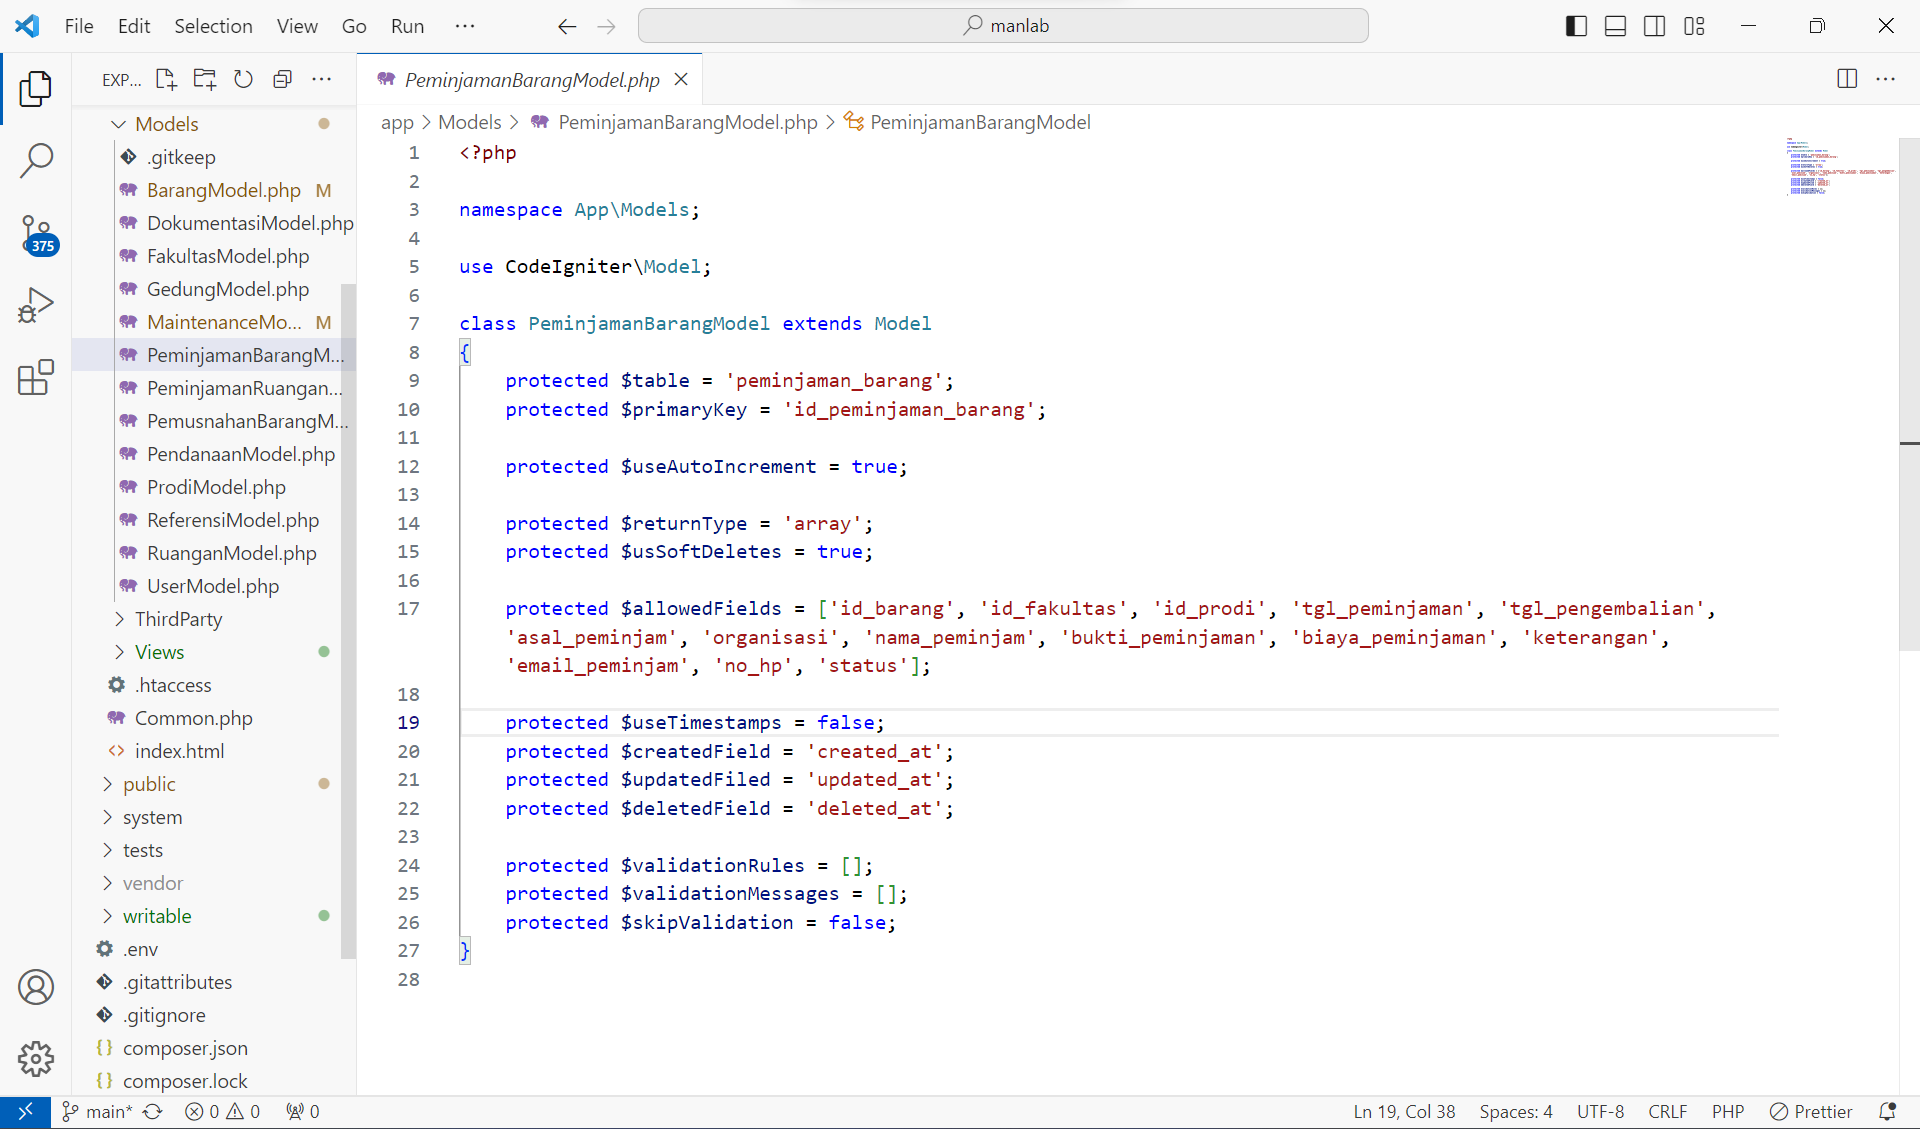
\includegraphics[width=0.82\linewidth]{konten//gambar/peminjaman barang model.png}
          \caption{Model Peminjaman Barang}
          \label{fig:enter-label}
        \end{figure}

  \item Model dalam implementasi sistem informasi inventaris laboratorium pada data peminjaman ruangan dapat dilihat pada Gambar 4.33.

        \begin{figure}
          \centering
          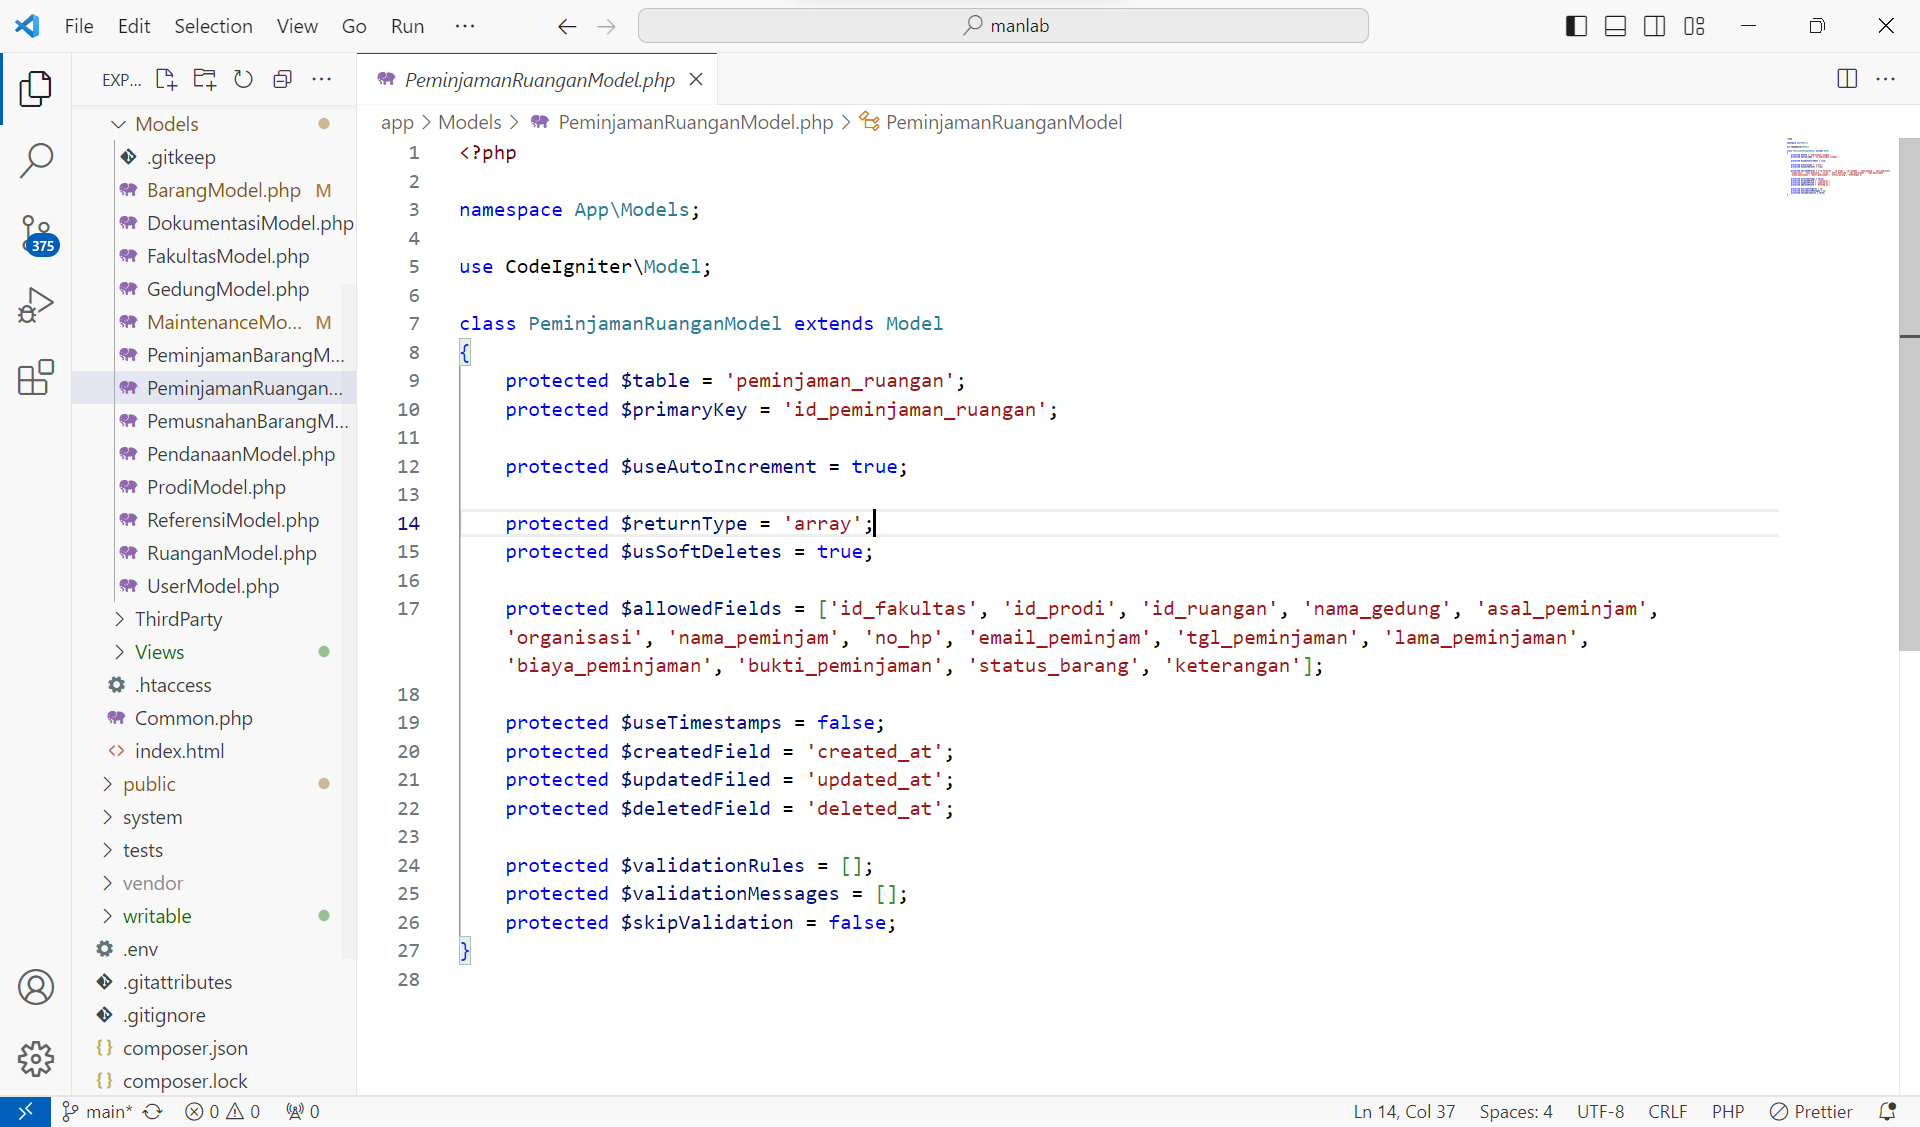
\includegraphics[width=0.82\linewidth]{konten//gambar/peminjaman ruangan model.png}
          \caption{Model Peminjaman Ruangan}
          \label{fig:enter-label}
        \end{figure}

  \item Model dalam implementasi sistem informasi inventaris laboratorium pada data pemusnahan barang dapat dilihat pada Gambar 4.34.

        \begin{figure}
          \centering
          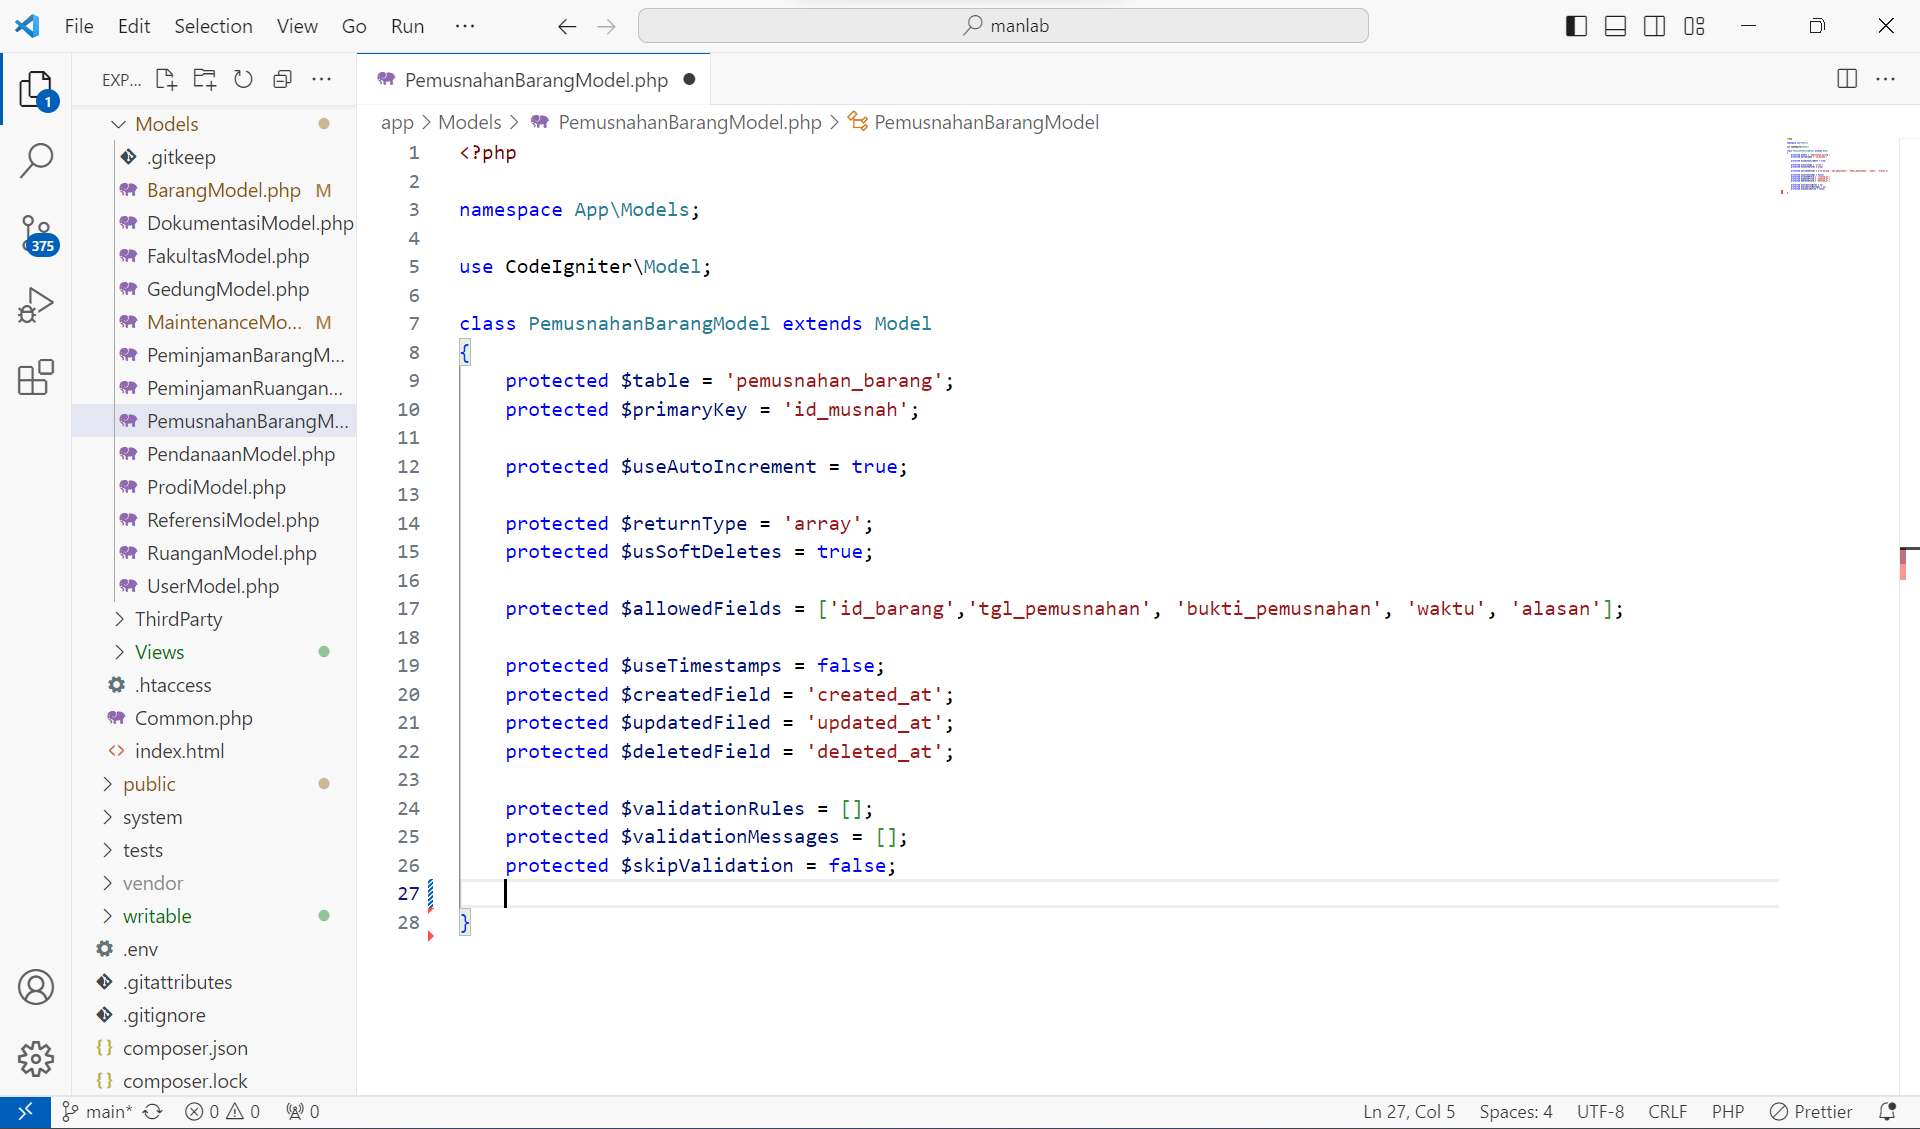
\includegraphics[width=0.82\linewidth]{konten//gambar/pemusnahan barang model.png}
          \caption{Model Pemusnahan Barang}
          \label{fig:enter-label}
        \end{figure}

  \item Model dalam implementasi sistem informasi inventaris laboratorium pada data pendanaan dapat dilihat pada Gambar 4.35.

        \begin{figure}
          \centering
          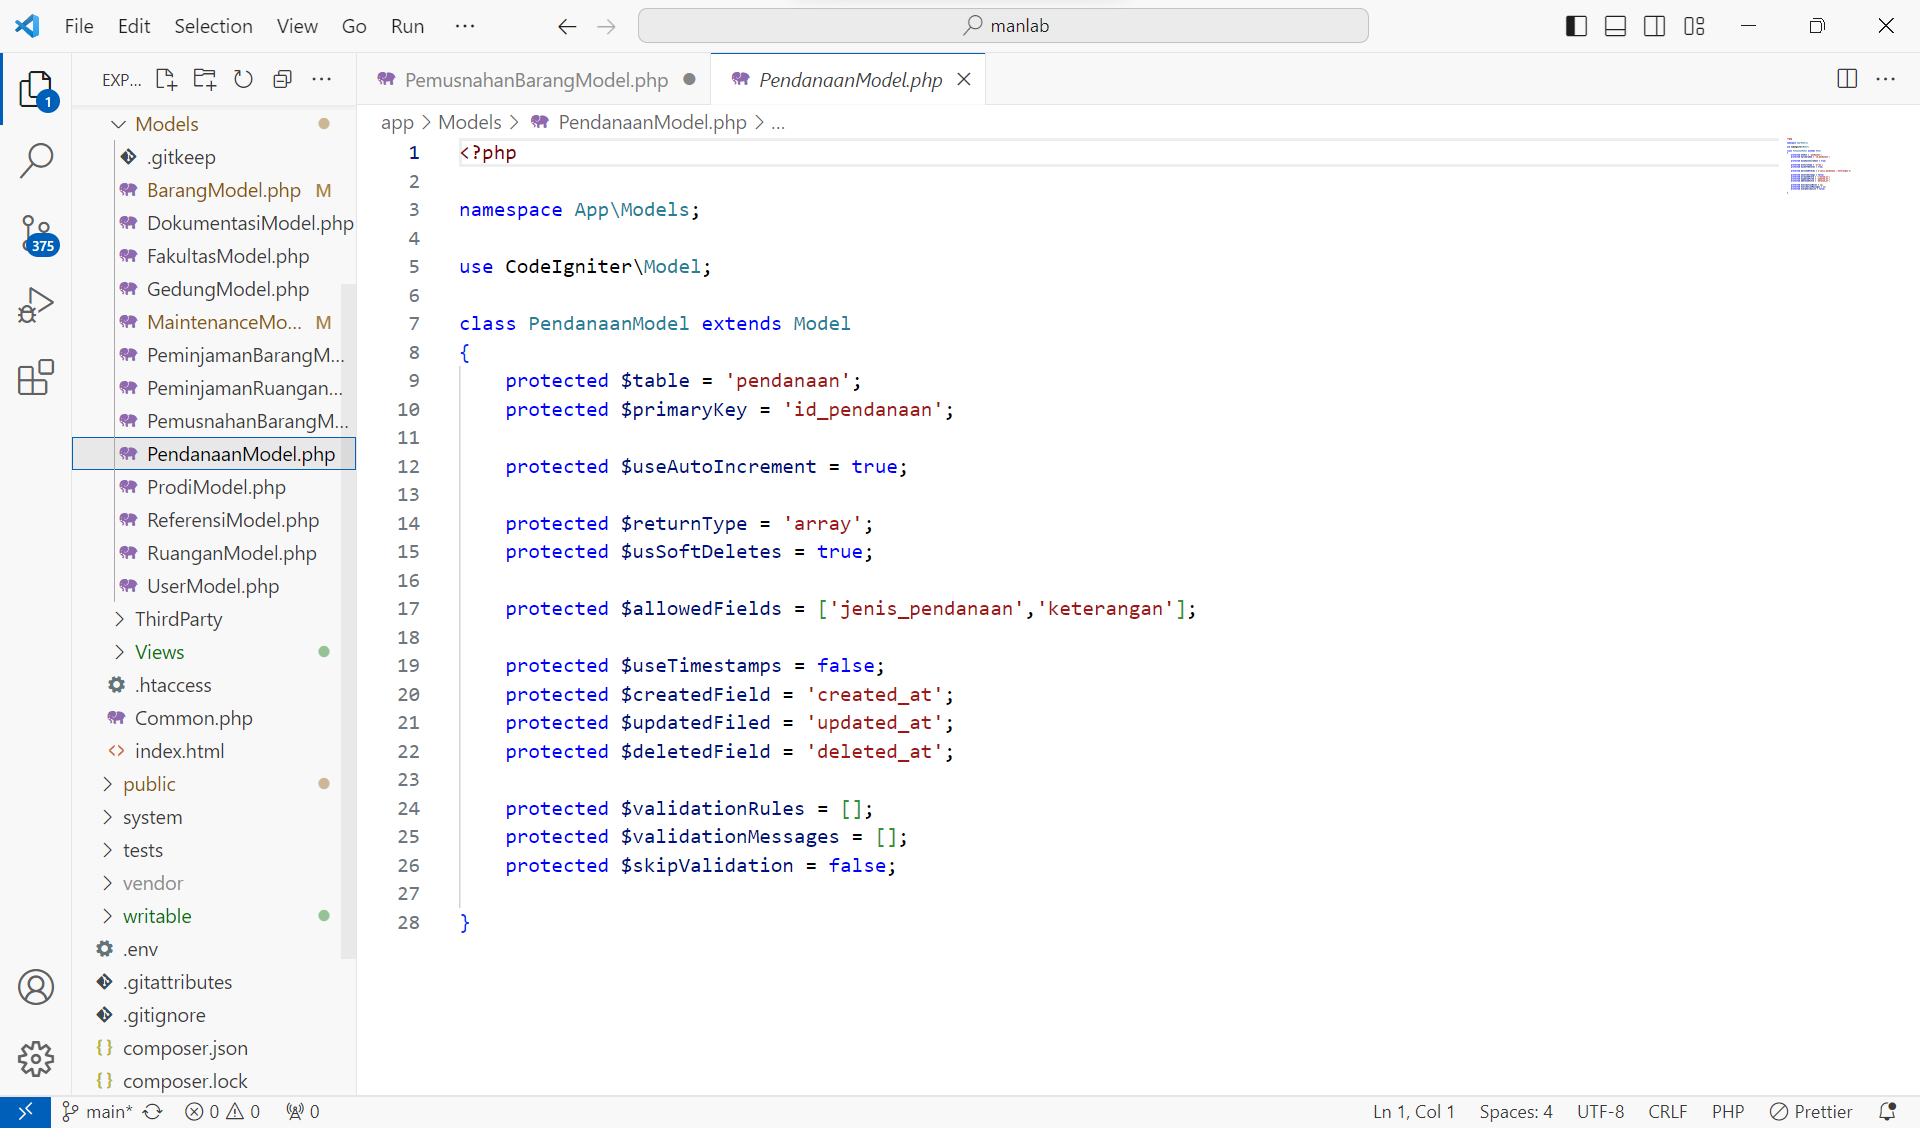
\includegraphics[width=0.82\linewidth]{konten//gambar/pendanaan model.png}
          \caption{Model Pendanaan}
          \label{fig:enter-label}
        \end{figure}

  \item Model dalam implementasi sistem informasi inventaris laboratorium pada data prodi dapat dilihat pada Gambar 4.36.

        \begin{figure}
          \centering
          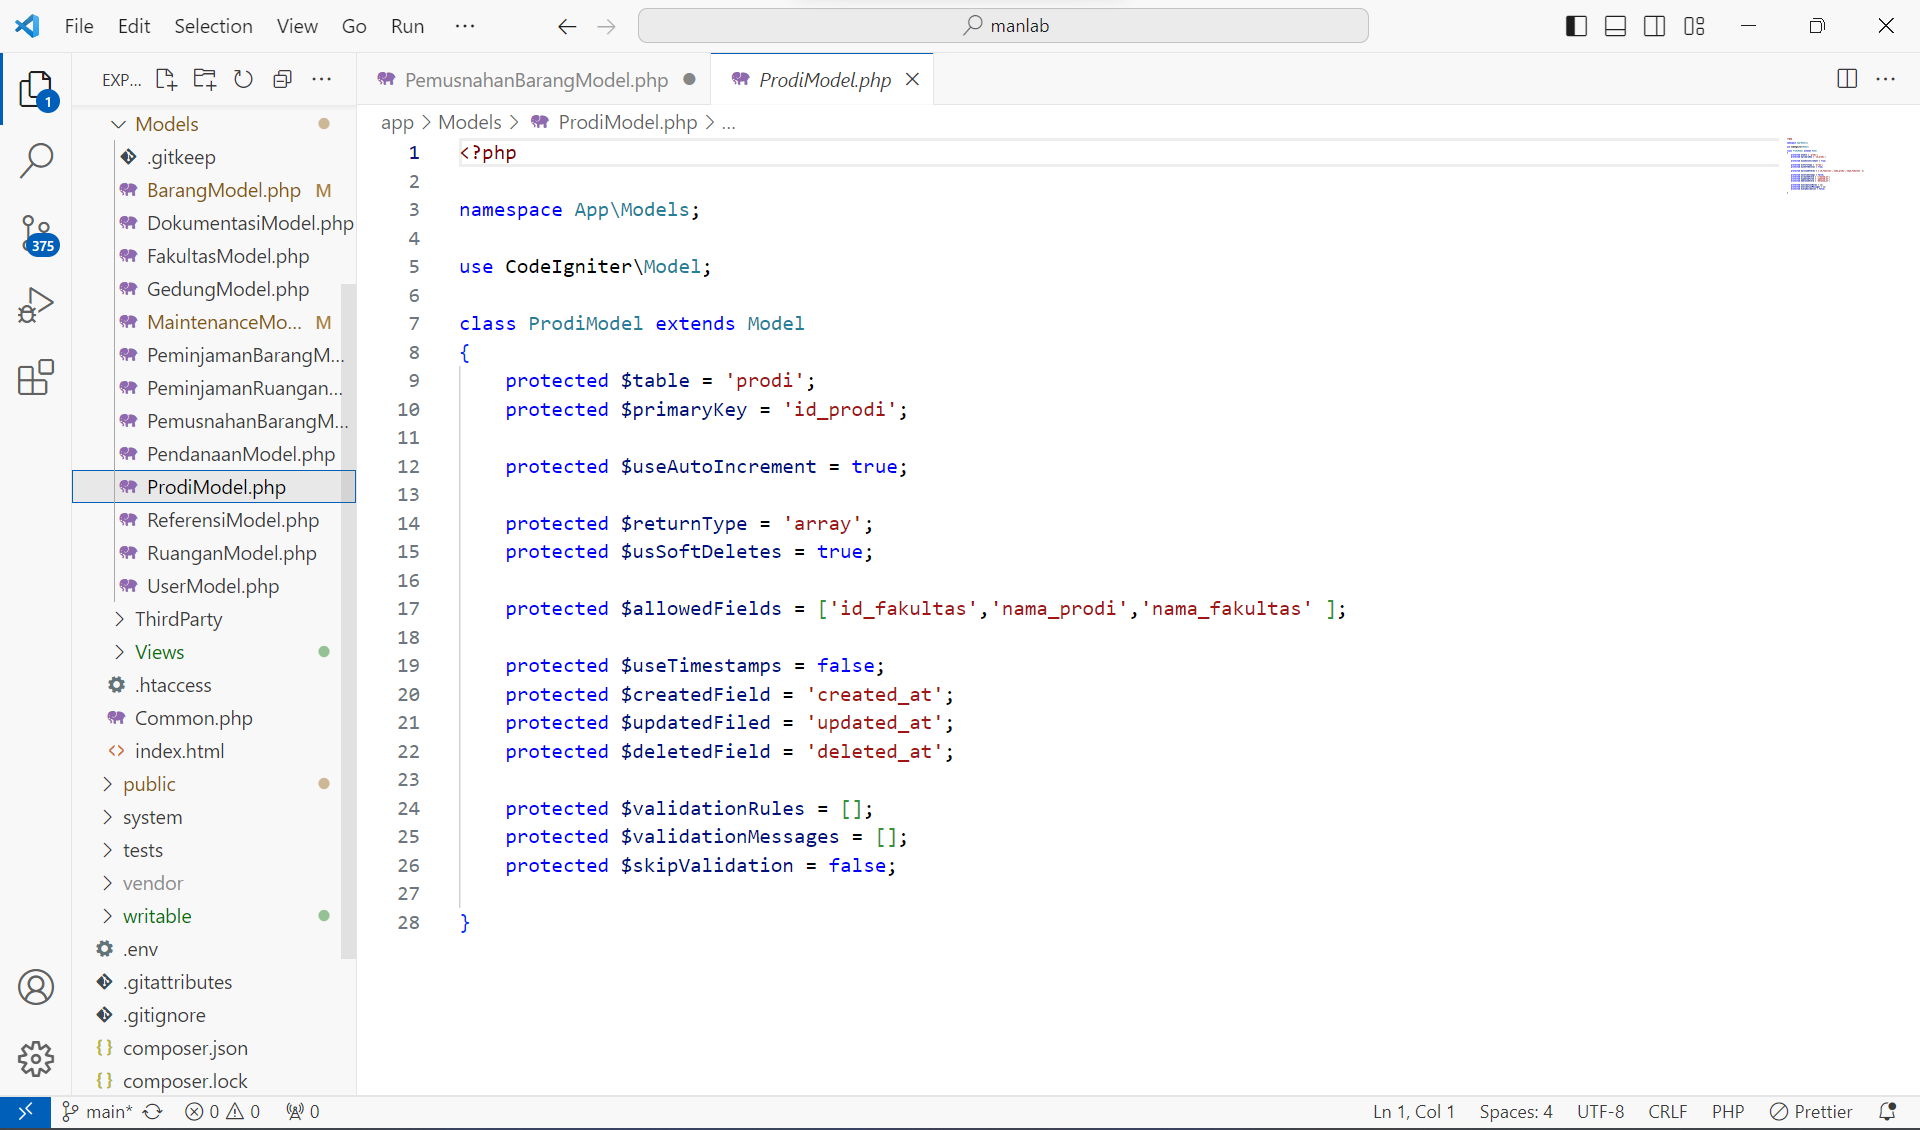
\includegraphics[width=0.82\linewidth]{konten//gambar/prodi model.png}
          \caption{Model Prodi}
          \label{fig:enter-label}
        \end{figure}

  \item Model dalam implementasi sistem informasi inventaris laboratorium pada data referensi dapat dilihat pada Gambar 4.37.

        \begin{figure}
          \centering
          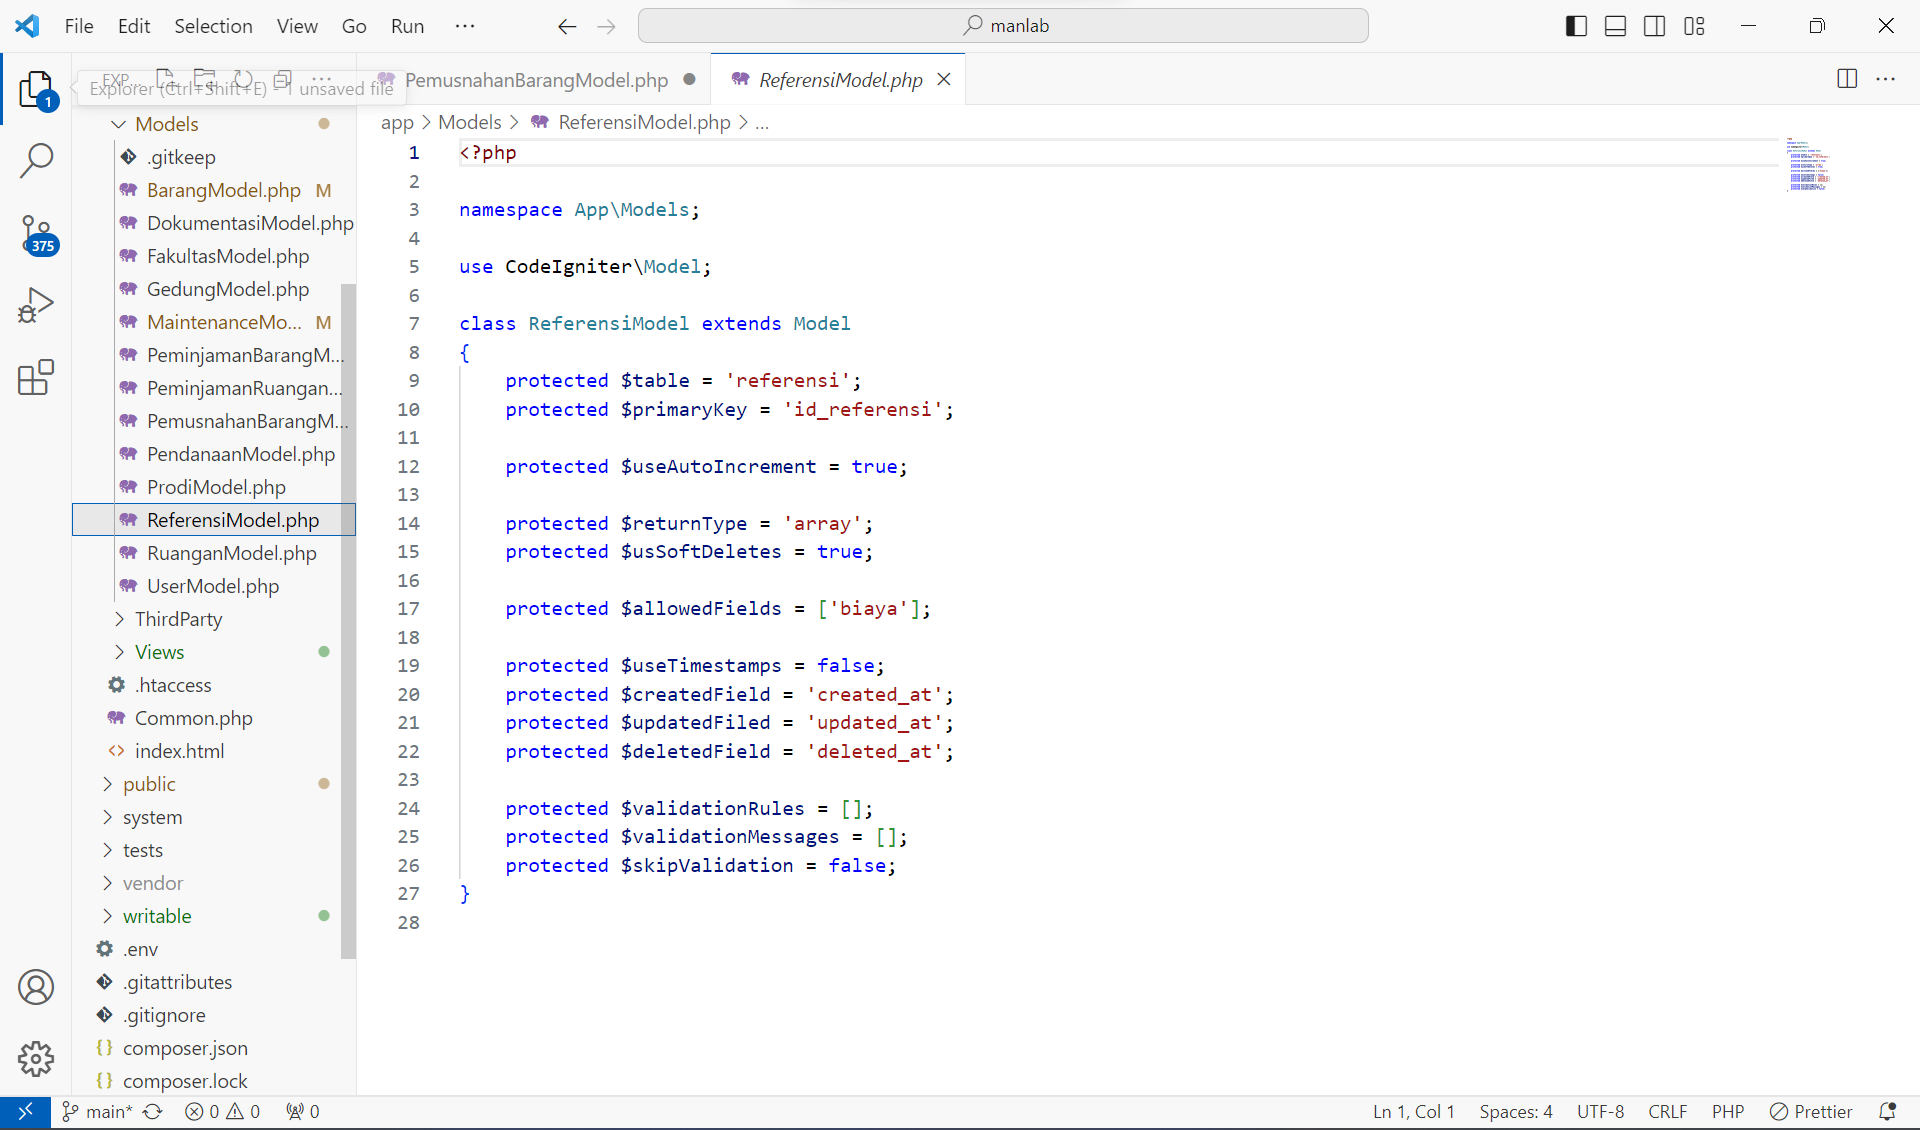
\includegraphics[width=0.82\linewidth]{konten//gambar/referensi model.png}
          \caption{Model Referensi}
          \label{fig:enter-label}
        \end{figure}

  \item Model dalam implementasi sistem informasi inventaris laboratorium pada data ruangan dapat dilihat pada Gambar 4.38.

        \begin{figure}
          \centering
          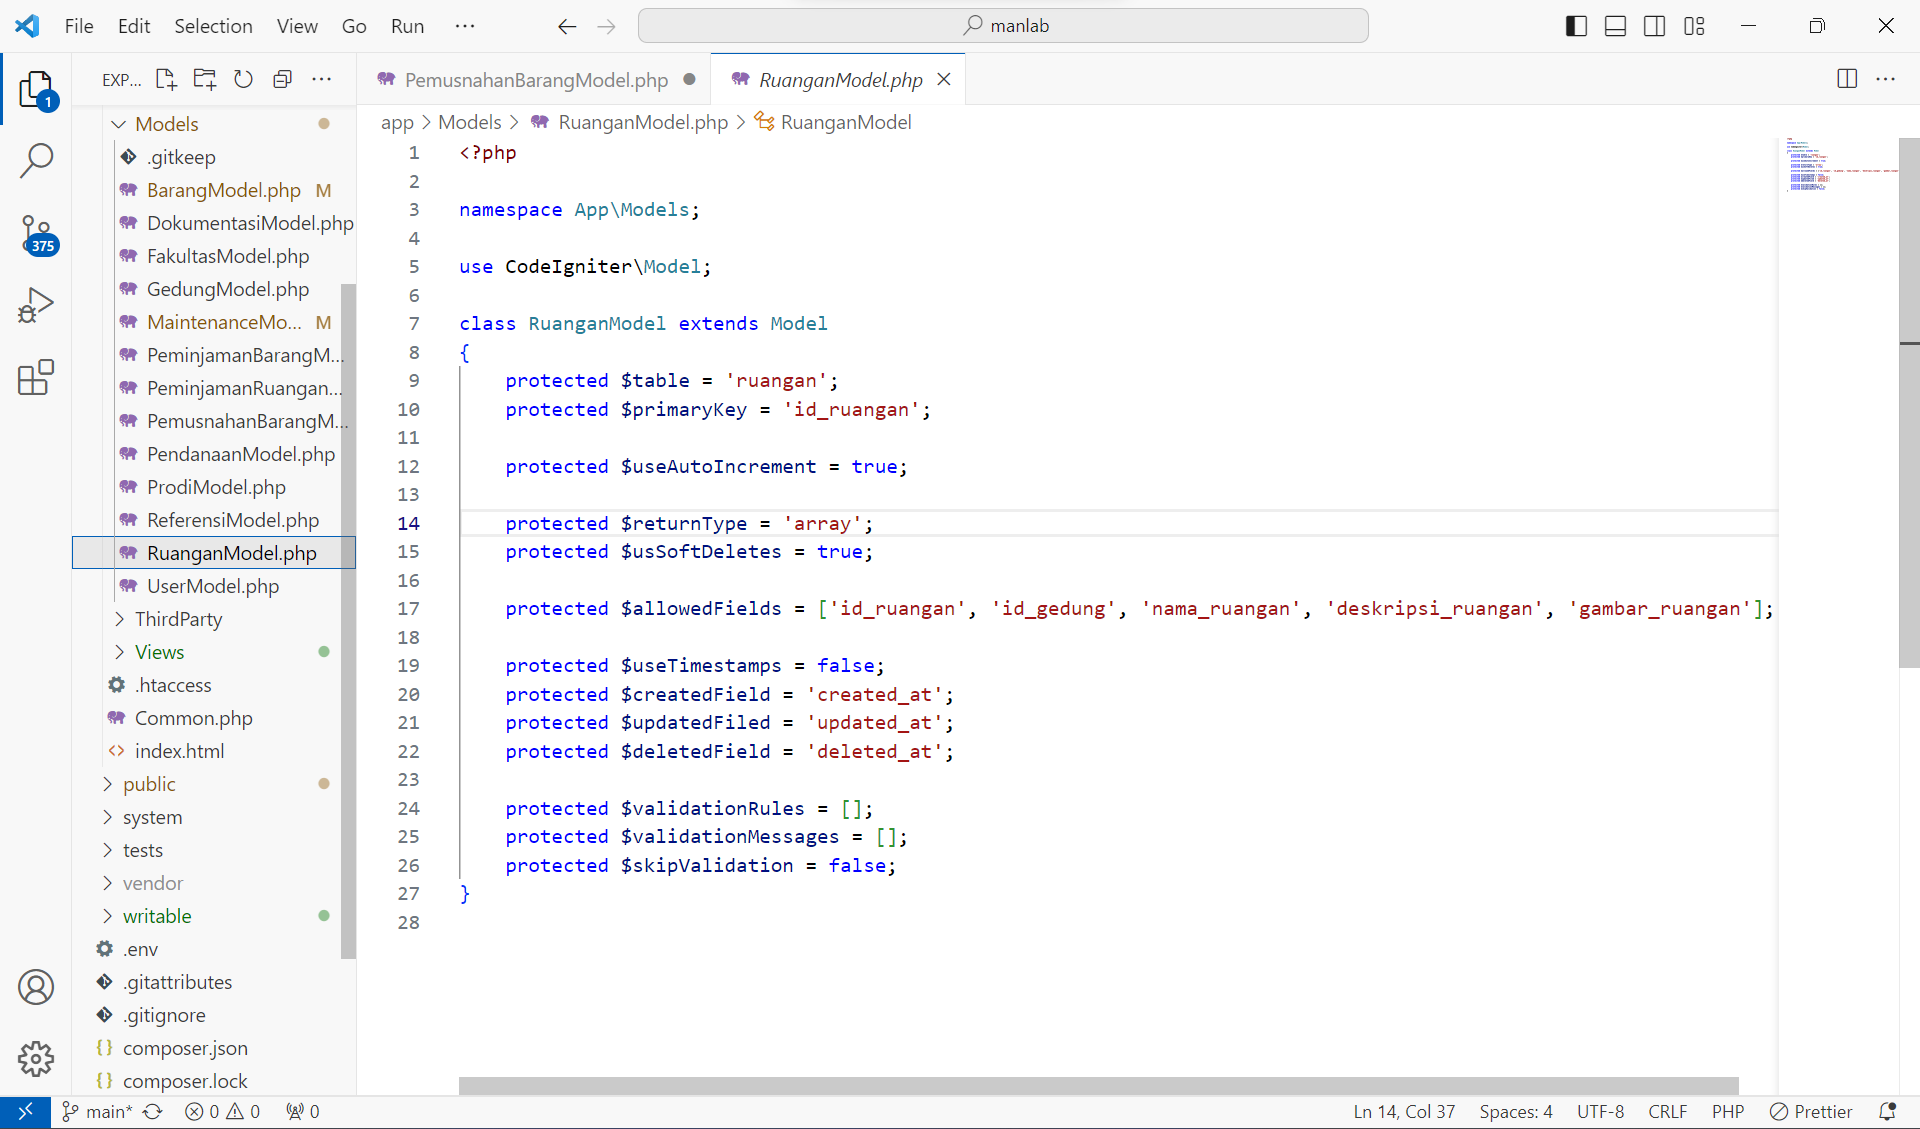
\includegraphics[width=0.82\linewidth]{konten//gambar/ruangan model.png}
          \caption{Model Ruangan}
          \label{fig:enter-label}
        \end{figure}

  \item Model dalam implementasi sistem informasi inventaris laboratorium pada data \textit{user} dapat dilihat pada Gambar 4.39.

        \begin{figure}
          \centering
          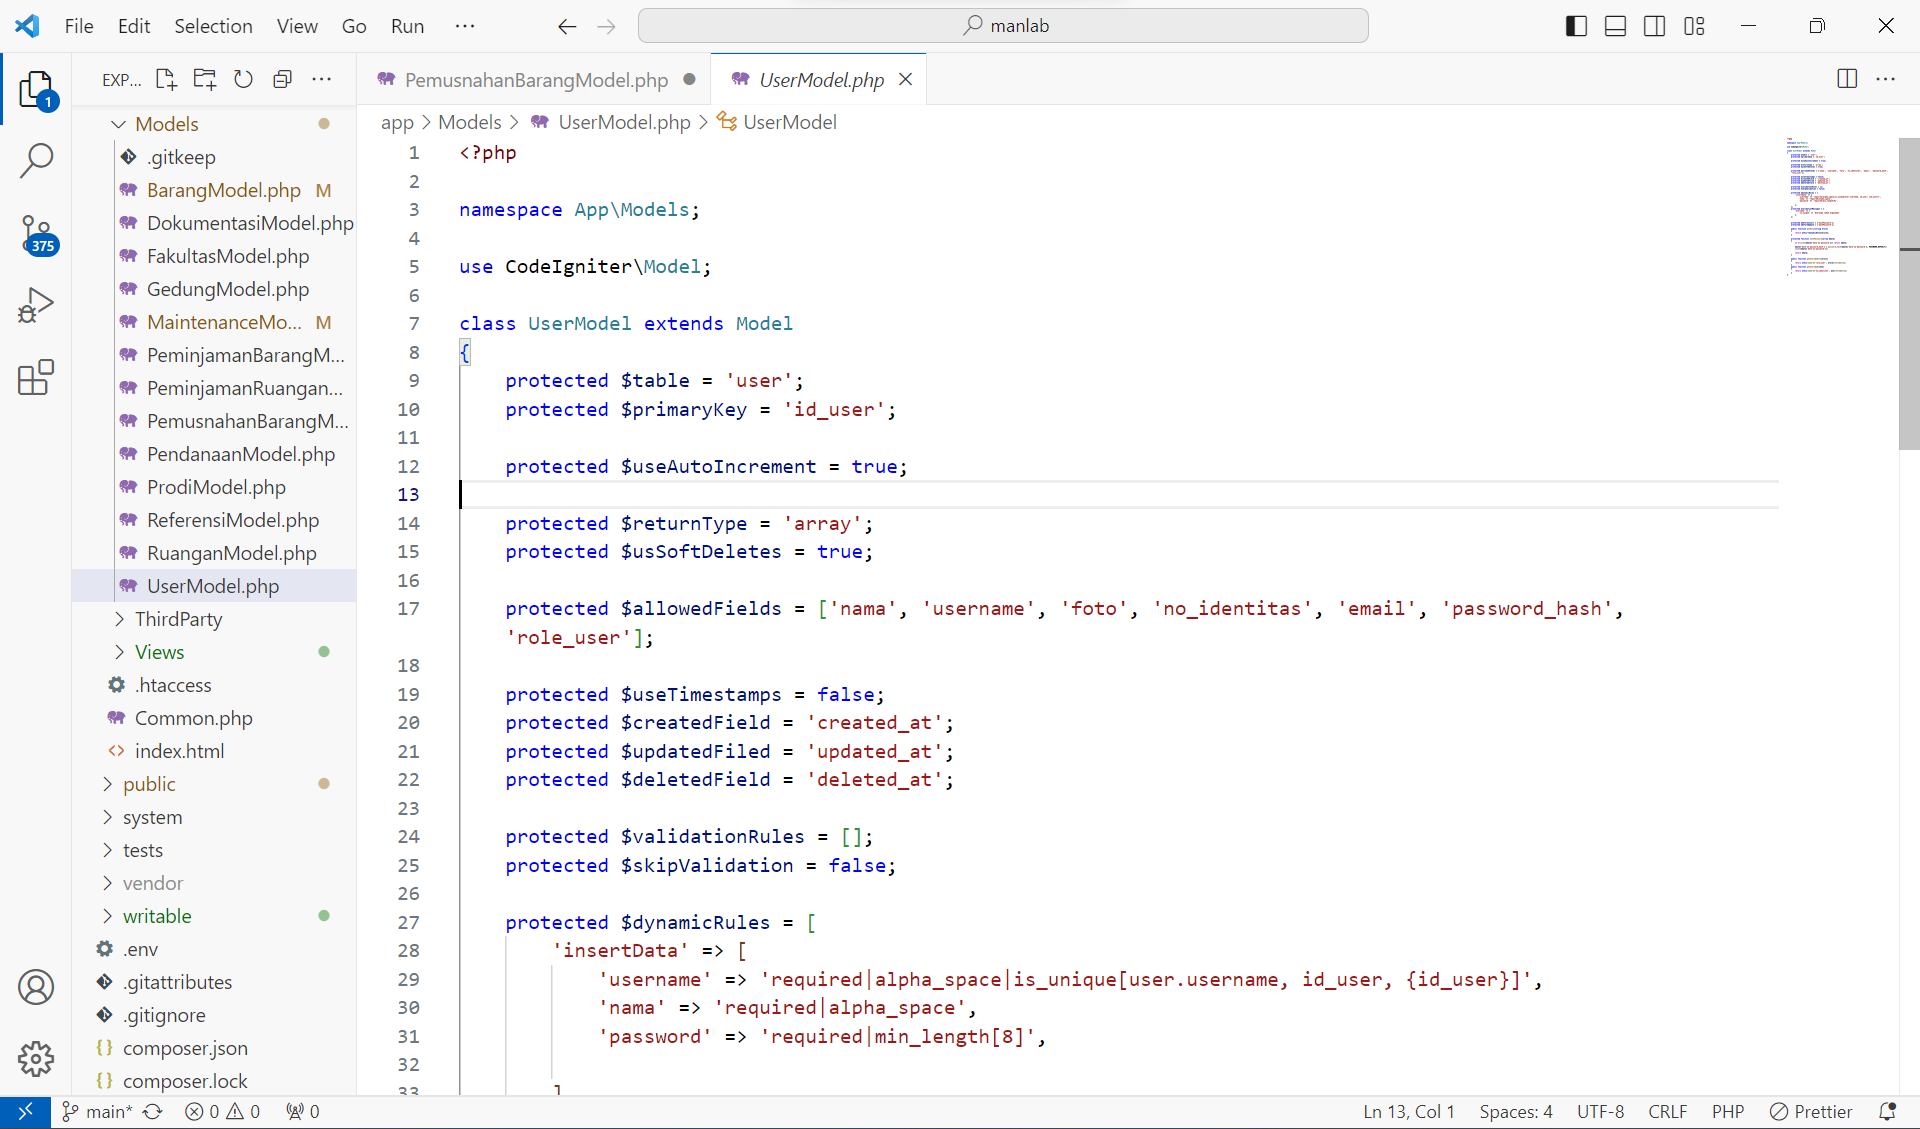
\includegraphics[width=0.82\linewidth]{konten//gambar/user model.png}
          \caption{Model \textit{User}}
          \label{fig:enter-label}
        \end{figure}

\end{enumerate}

\subsection{\textit{View}}
\textit{View }adalah komponen yang menampilkan antarmuka pengguna dan menampilkan data dari Model. \textit{View} mengamati perubahan pada Model dan \textit{Controller}, dan diperbarui sesuai keadaan terkini. Penggunaan \textit{View} memisahkan tugas penyajian dan manajemen data dalam aplikasi, yang memberikan fleksibilitas dan pemeliharaan yang lebih baik \cite{firdaus2020rancang}.

\begin{enumerate}
  \item \textit{View} dalam implementasi sistem informasi inventaris laboratorium pada data barang dapat dilihat pada Gambar 4.40.
        \begin{figure}
          \centering
          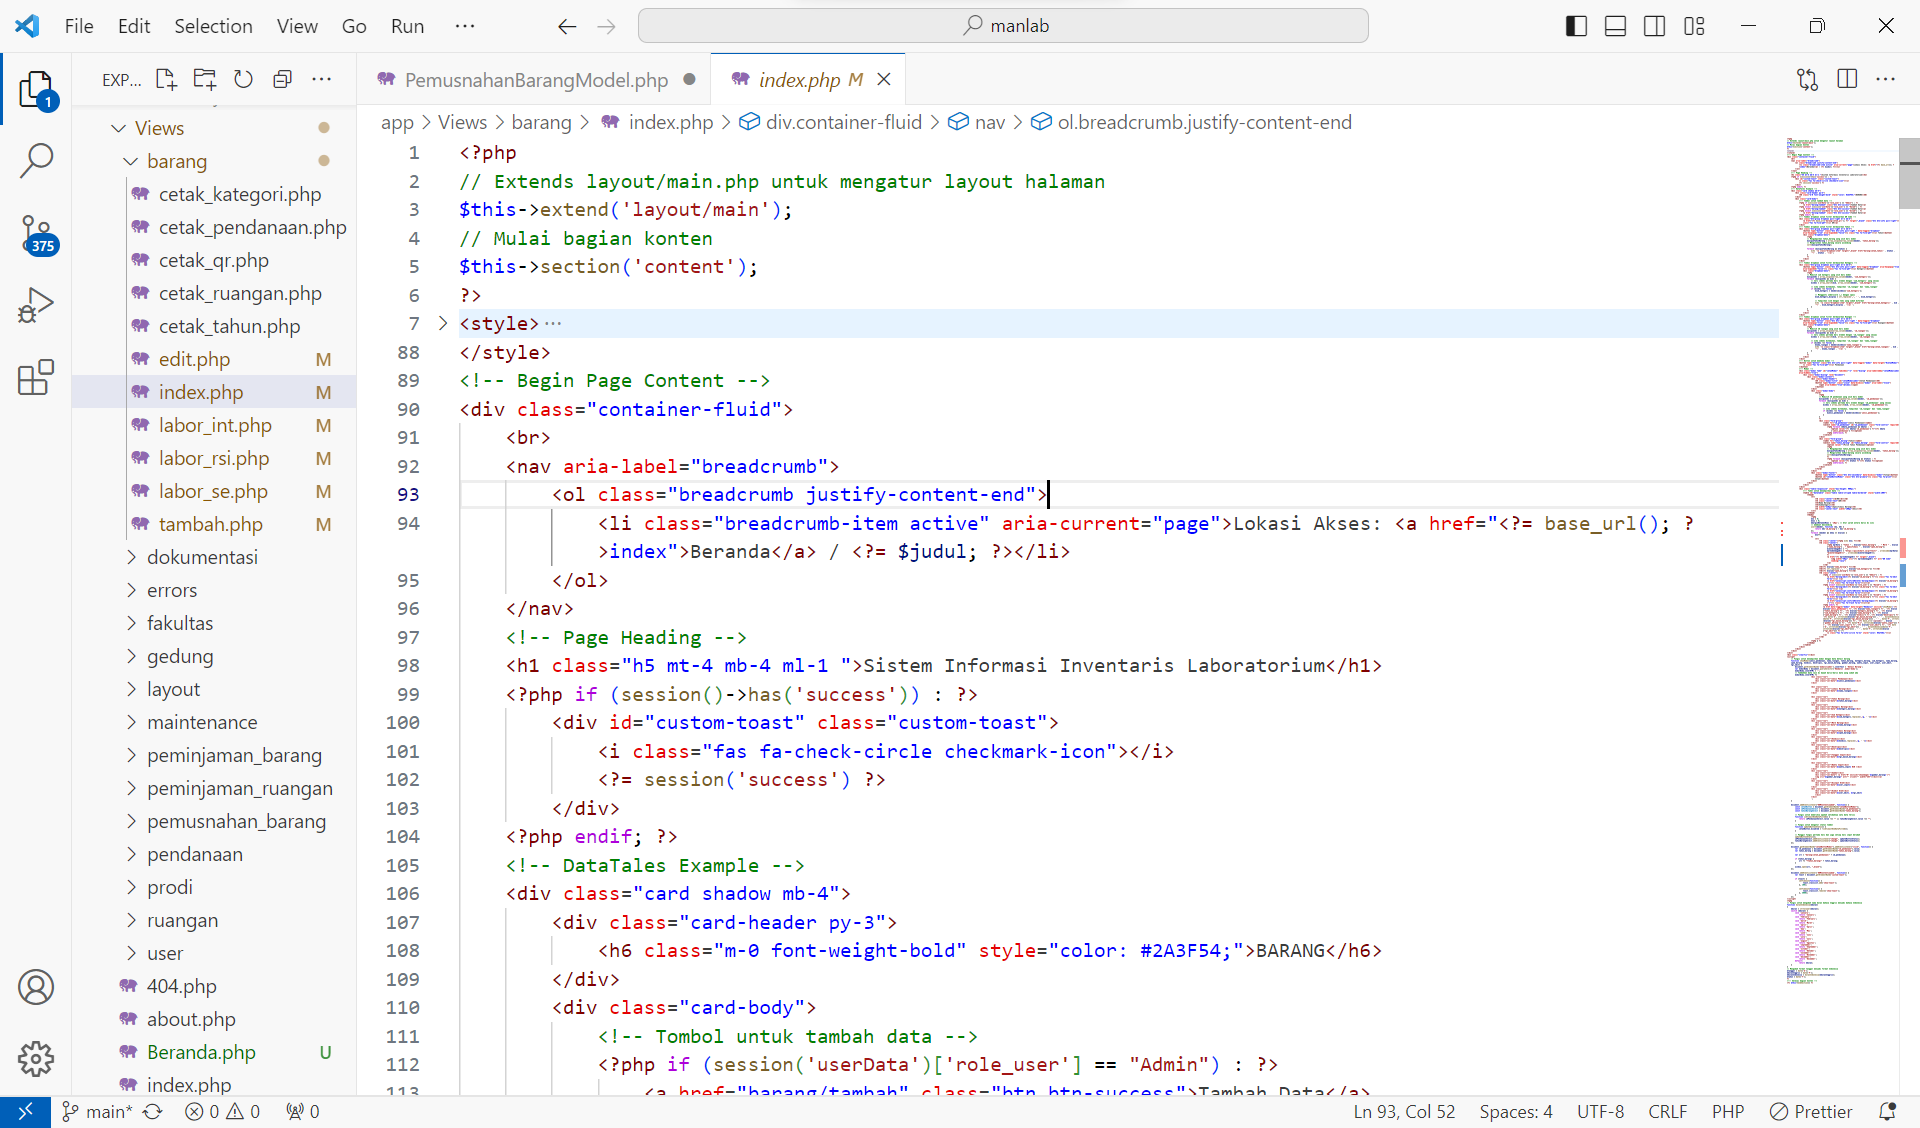
\includegraphics[width=0.82\linewidth]{konten//gambar/view barang.png}
          \caption{\textit{View} Barang}
          \label{fig:enter-label}
        \end{figure}

  \item \textit{View} dalam implementasi sistem informasi inventaris laboratorium pada data dokumentasi dapat dilihat pada Gambar 4.41.
        \begin{figure}
          \centering
          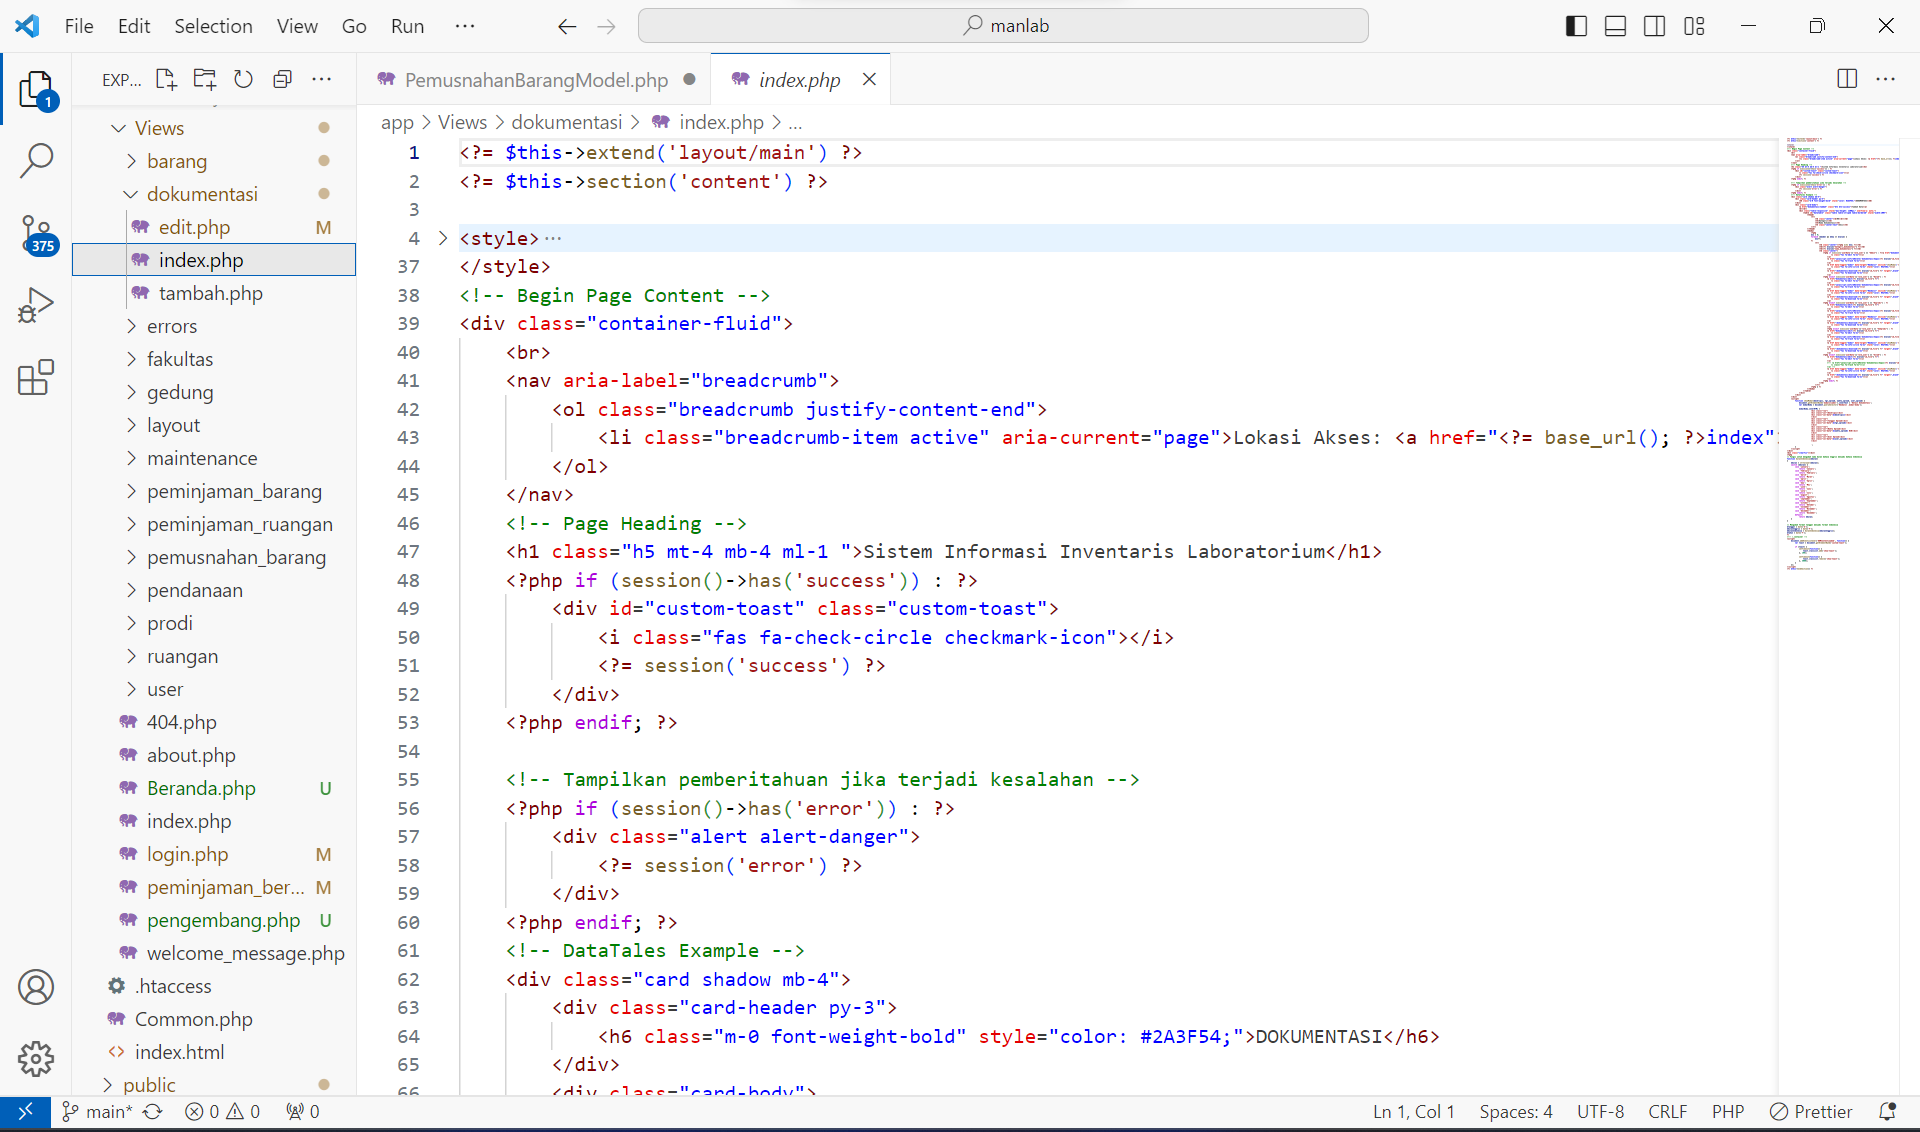
\includegraphics[width=0.82\linewidth]{konten//gambar/view dokumentasi.png}
          \caption{\textit{View} Dokumentasi}
          \label{fig:enter-label}
        \end{figure}

  \item \textit{View} dalam implementasi sistem informasi inventaris laboratorium pada data fakultas dapat dilihat pada Gambar 4.42.
        \begin{figure}
          \centering
          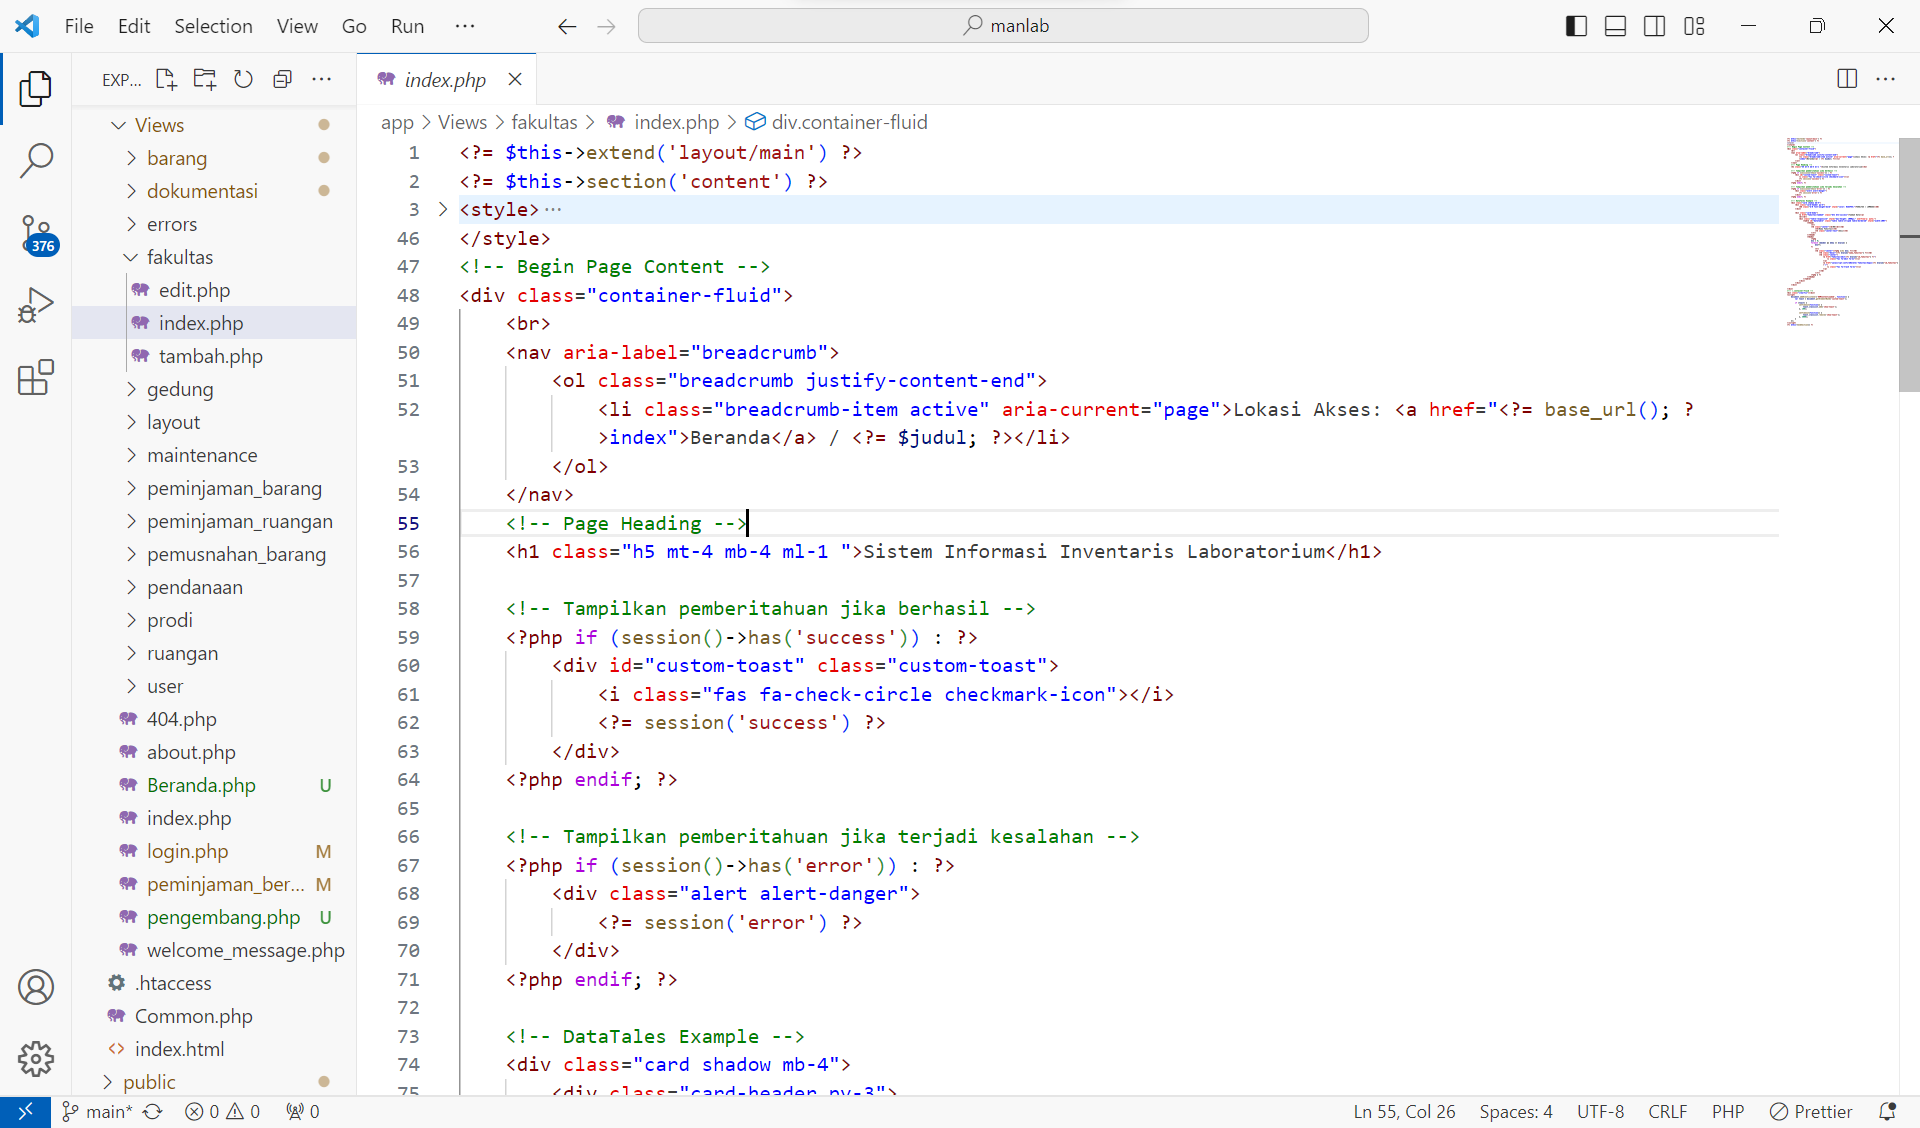
\includegraphics[width=0.82\linewidth]{konten//gambar/view fakultas.png}
          \caption{\textit{View} Fakultas}
          \label{fig:enter-label}
        \end{figure}

  \item \textit{View} dalam implementasi sistem informasi inventaris laboratorium pada data gedung dapat dilihat pada Gambar 4.43.
        \begin{figure}
          \centering
          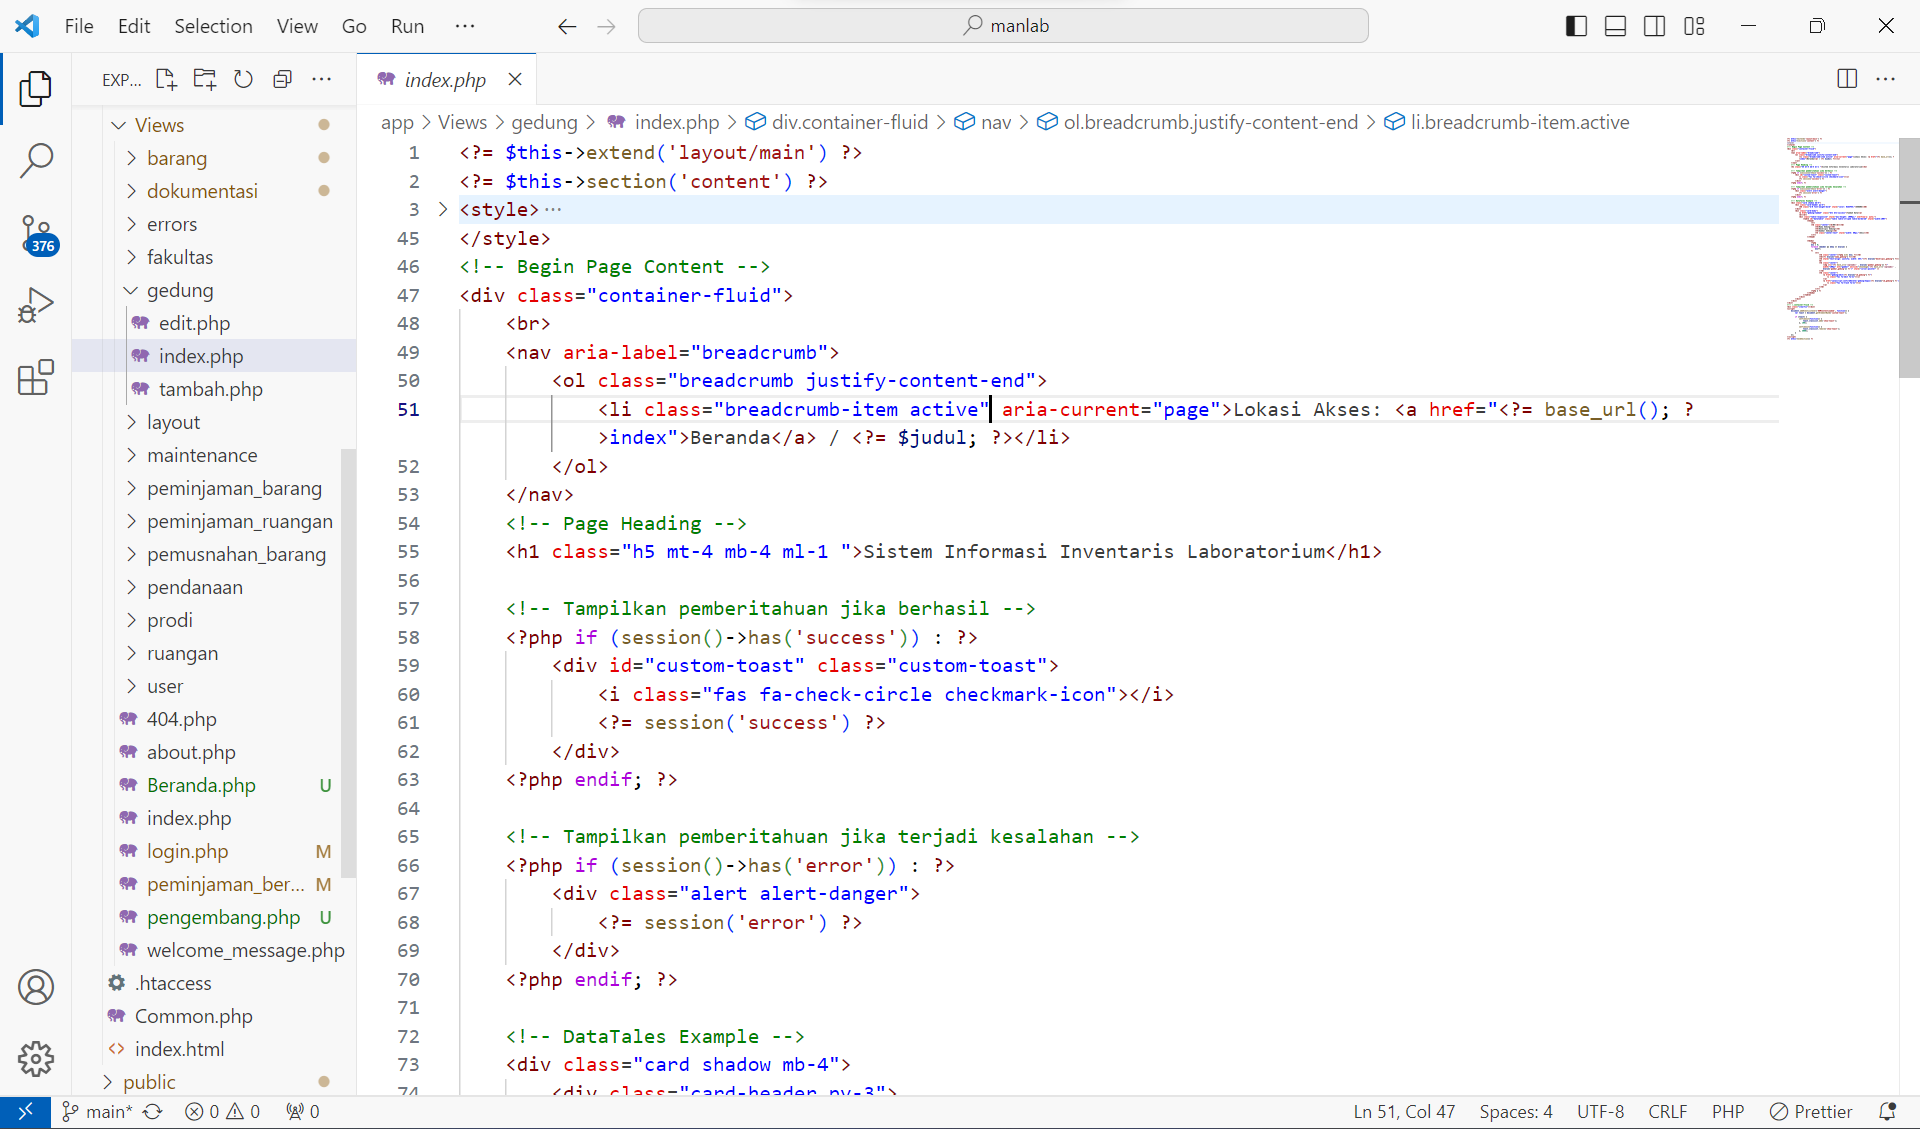
\includegraphics[width=0.82\linewidth]{konten//gambar/view gedung.png}
          \caption{\textit{View} Gedung}
          \label{fig:enter-label}
        \end{figure}

  \item \textit{View} dalam implementasi sistem informasi inventaris laboratorium pada data \textit{maintenance} dapat dilihat pada Gambar 4.44.
        \begin{figure}
          \centering
          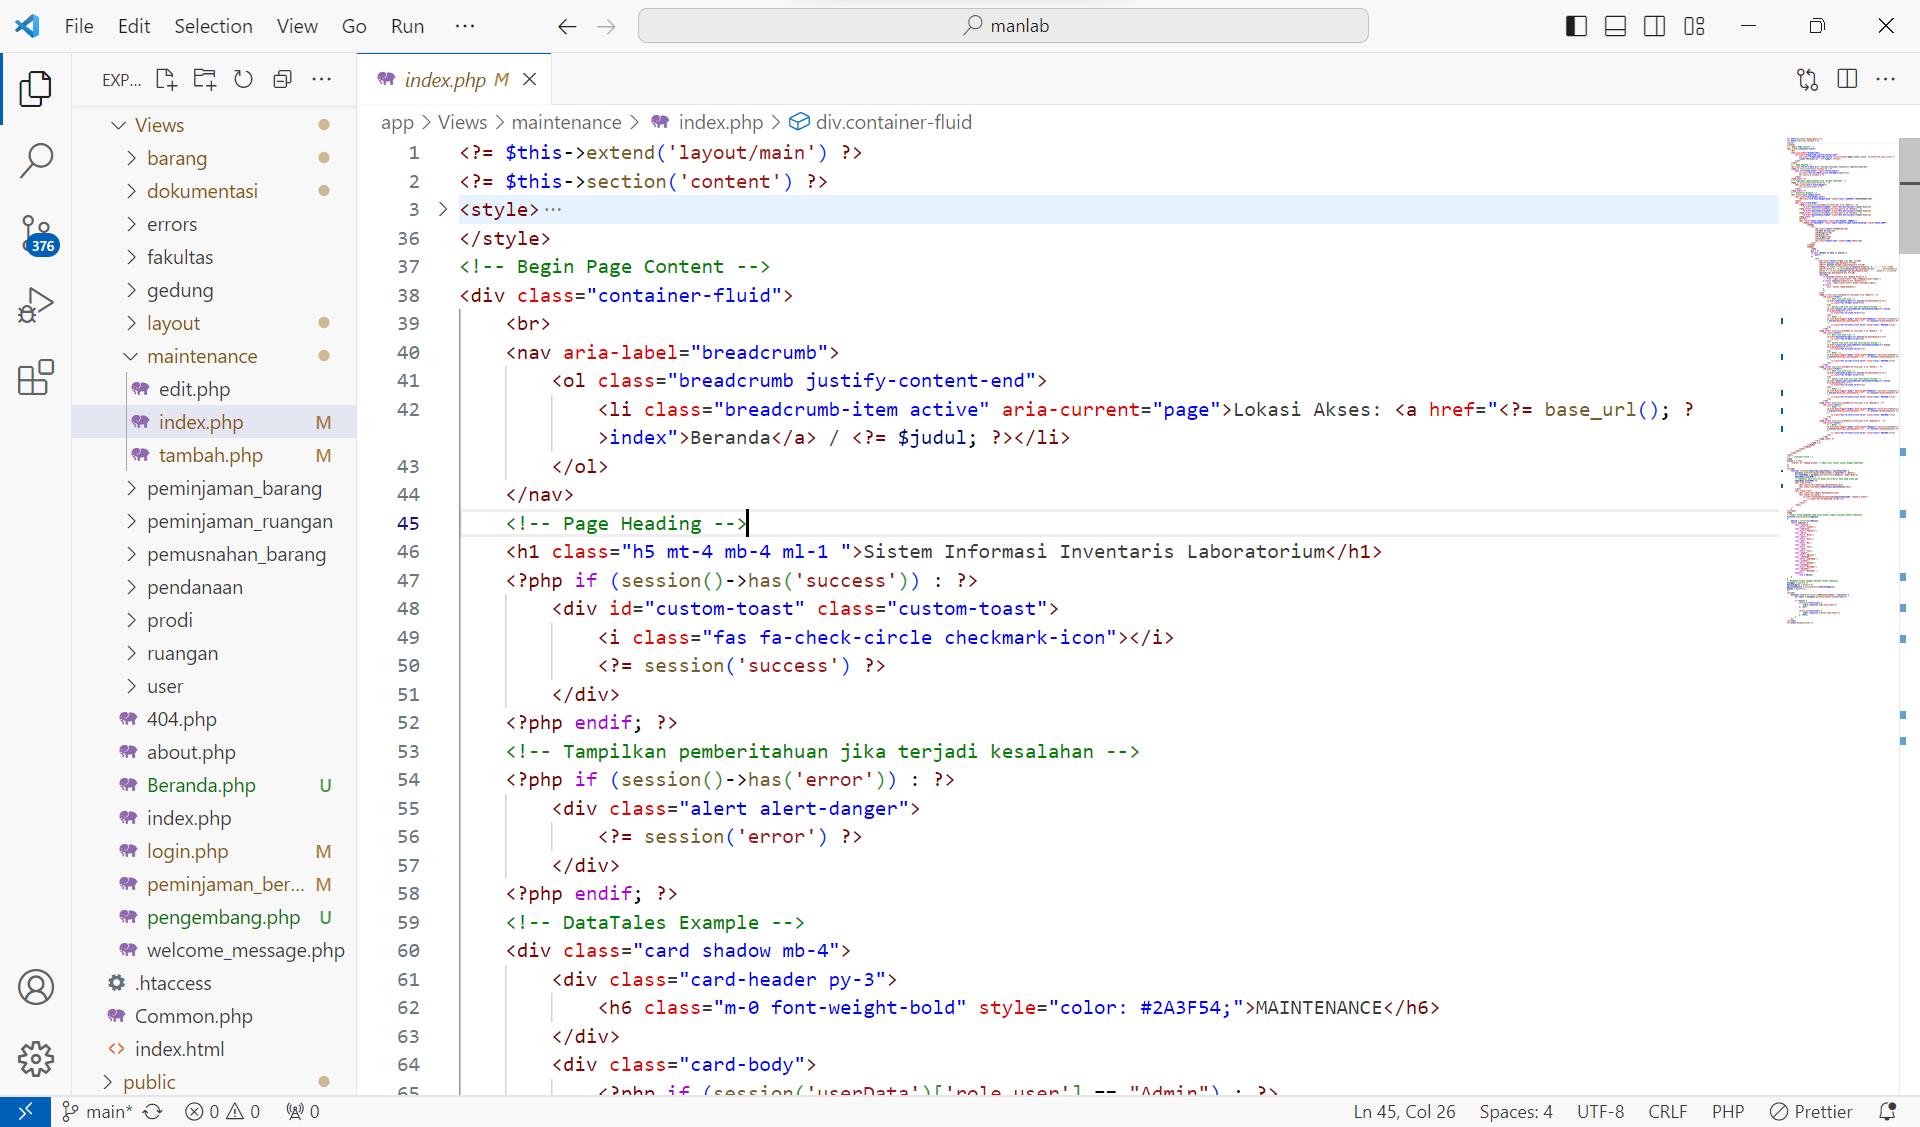
\includegraphics[width=0.82\linewidth]{konten//gambar/view maintenance.png}
          \caption{\textit{View Maintenance}}
          \label{fig:enter-label}
        \end{figure}

  \item \textit{View} dalam implementasi sistem informasi inventaris laboratorium pada data peminjaman barang dapat dilihat pada Gambar 4.45.
        \begin{figure}
          \centering
          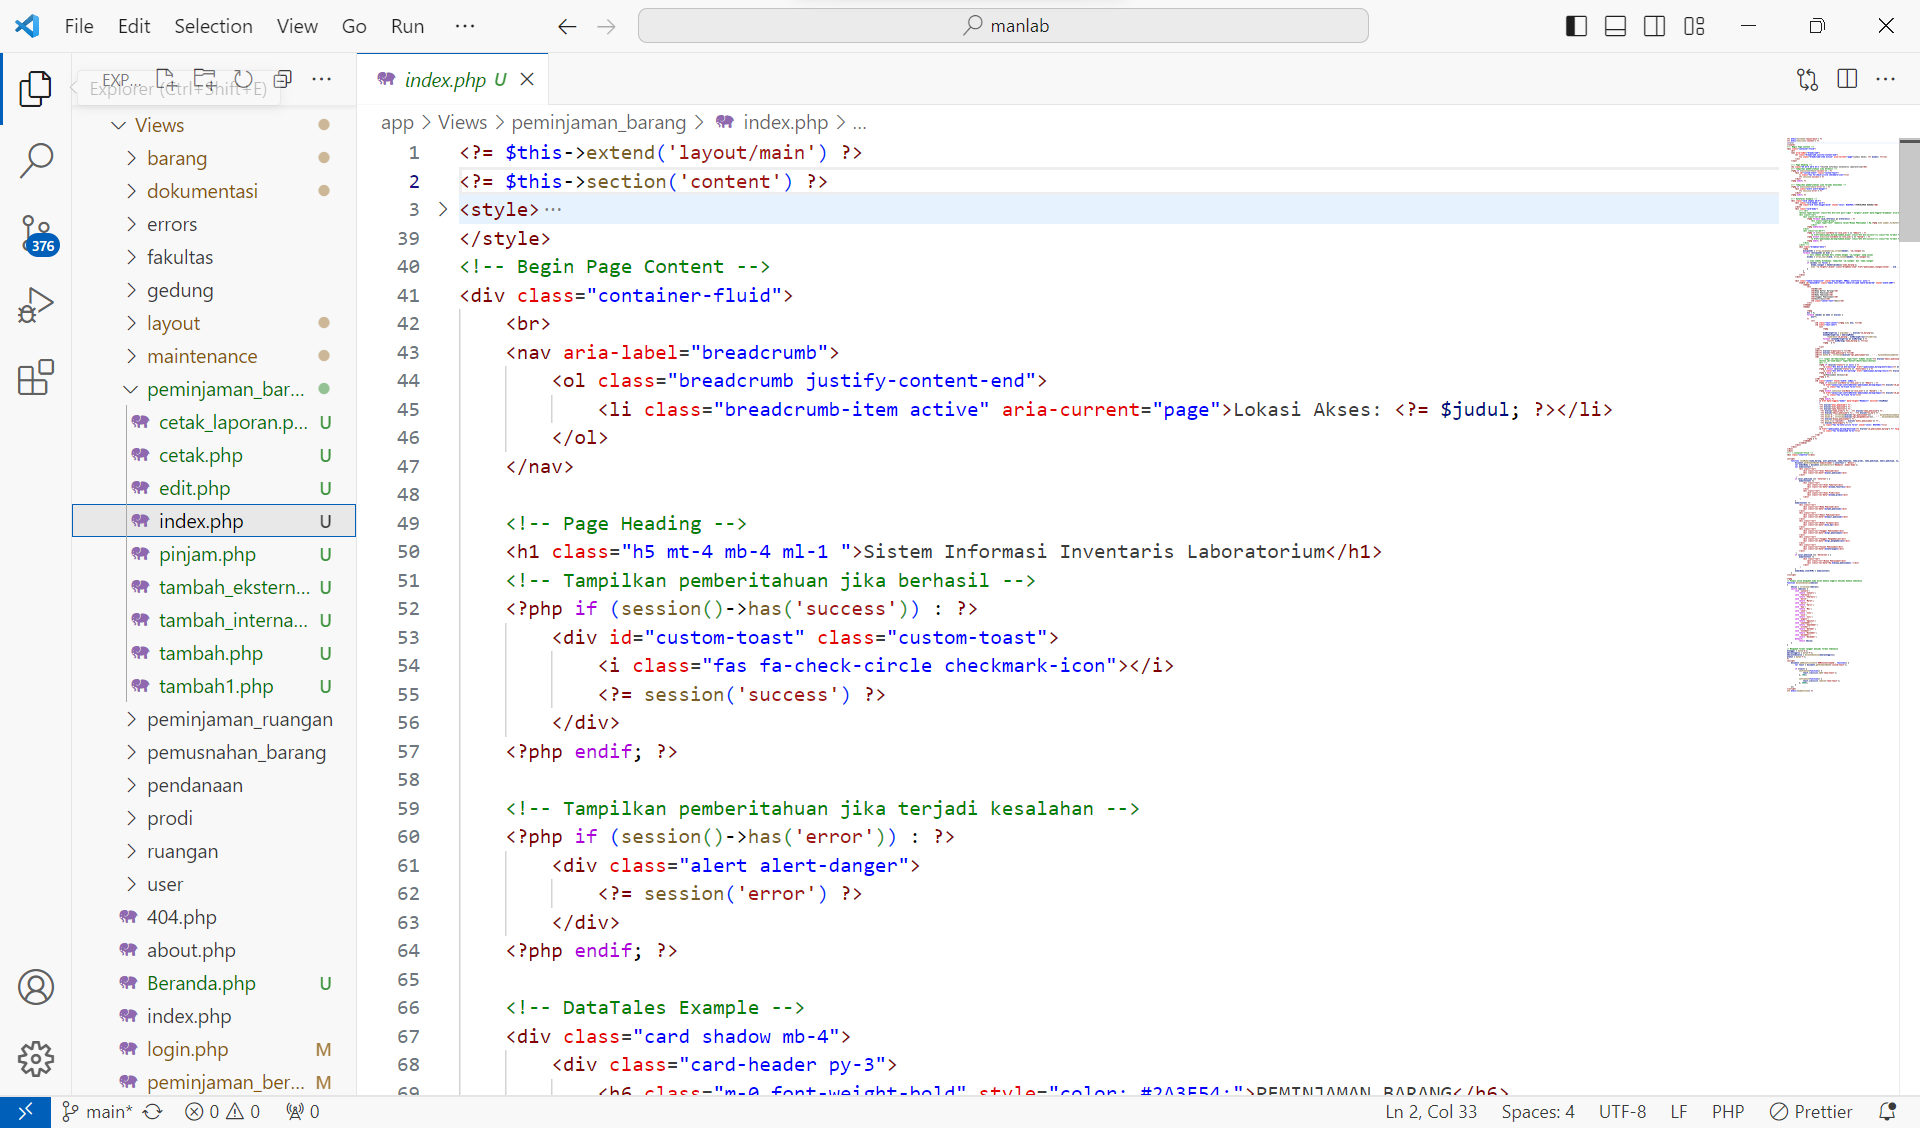
\includegraphics[width=0.82\linewidth]{konten//gambar/view peminjaman_barang.png}
          \caption{\textit{View} Peminjaman Barang}
          \label{fig:enter-label}
        \end{figure}

  \item \textit{View} dalam implementasi sistem informasi inventaris laboratorium pada data peminjaman ruangan dapat dilihat pada Gambar 4.46.
        \begin{figure}
          \centering
          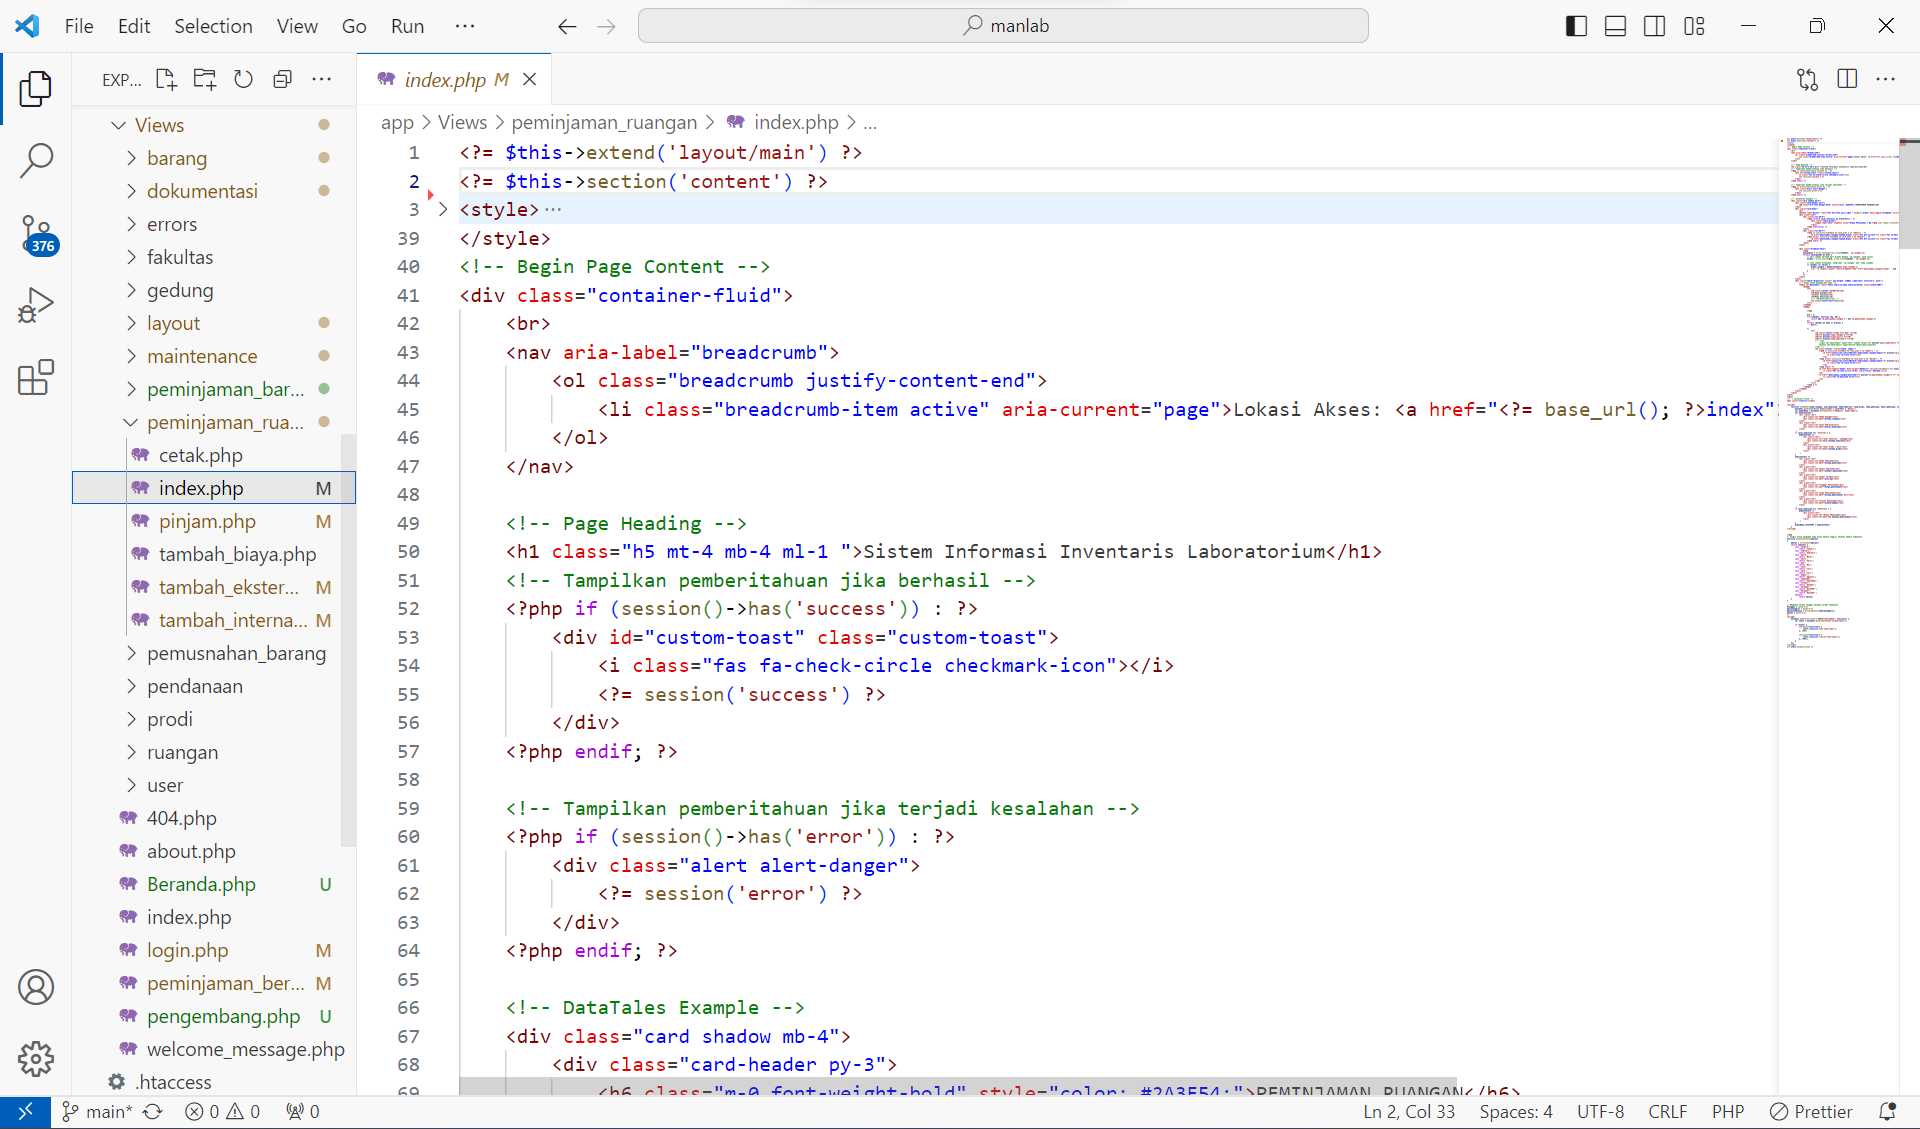
\includegraphics[width=0.82\linewidth]{konten//gambar/view peminjaman_ruangan.png}
          \caption{\textit{View} Peminjaman Ruangan}
          \label{fig:enter-label}
        \end{figure}

  \item \textit{View} dalam implementasi sistem informasi inventaris laboratorium pada data pemusnahan barang dapat dilihat pada Gambar 4.47.
        \begin{figure}
          \centering
          \includegraphics[width=0.82\linewidth]{konten//gambar/view pemusnahan_barang.png}
          \caption{\textit{View} Pemusnahan Barang}
          \label{fig:enter-label}
        \end{figure}

  \item \textit{View} dalam implementasi sistem informasi inventaris laboratorium pada data pendanaan dapat dilihat pada Gambar 4.48.
        \begin{figure}
          \centering
          \includegraphics[width=0.82\linewidth]{konten//gambar/view pendanaan.png}
          \caption{\textit{View} Pendanaan}
          \label{fig:enter-label}
        \end{figure}

  \item \textit{View} dalam implementasi sistem informasi inventaris laboratorium pada data prodi dapat dilihat pada Gambar 4.49.
        \begin{figure}
          \centering
          \includegraphics[width=0.82\linewidth]{konten//gambar/view prodi.png}
          \caption{\textit{View} Prodi}
          \label{fig:enter-label}
        \end{figure}

  \item \textit{View} dalam implementasi sistem informasi inventaris laboratorium pada data ruangan dapat dilihat pada Gambar 4.50.
        \begin{figure}
          \centering
          \includegraphics[width=0.82\linewidth]{konten//gambar/view ruangan.png}
          \caption{\textit{View} Ruangan}
          \label{fig:enter-label}
        \end{figure}

  \item \textit{View} dalam implementasi sistem informasi inventaris laboratorium pada data \textit{user} dapat dilihat pada Gambar 4.51.
        \begin{figure}
          \centering
          \includegraphics[width=0.82\linewidth]{konten//gambar/view user.png}
          \caption{\textit{View User}}
          \label{fig:enter-label}
        \end{figure}

\end{enumerate}

\subsection{\textit{Controller}}
\textit{Controller} adalah komponen yang bertanggung jawab untuk mengatur logika pengendalian atau interaksi antara Model (data), \textit{View} (tampilan), dan pengguna \cite{rahman2018perancangan}.

\begin{enumerate}
  \item \textit{Controller} dalam implementasi sistem informasi inventaris laboratorium pada data barang dapat dilihat pada Gambar 4.52.

        \begin{figure}
          \centering
          \includegraphics[width=0.82\linewidth]{konten//gambar/barang controller.png}
          \caption{\textit{Controller} Barang}
          \label{fig:enter-label}
        \end{figure}

  \item \textit{Controller} dalam implementasi sistem informasi inventaris laboratorium pada data dokumentasi dapat dilihat pada Gambar 4.53.

        \begin{figure}
          \centering
          \includegraphics[width=0.82\linewidth]{konten//gambar/dokumentasi controller.png}
          \caption{\textit{Controller} Dokumentasi}
          \label{fig:enter-label}
        \end{figure}

  \item \textit{Controller} dalam implementasi sistem informasi inventaris laboratorium pada data fakultas dapat dilihat pada Gambar 4.54.

        \begin{figure}
          \centering
          \includegraphics[width=0.82\linewidth]{konten//gambar/fakultas controller.png}
          \caption{\textit{Controller} Fakultas}
          \label{fig:enter-label}
        \end{figure}

  \item \textit{Controller} dalam implementasi sistem informasi inventaris laboratorium pada data gedung dapat dilihat pada Gambar 4.55.

        \begin{figure}
          \centering
          \includegraphics[width=0.82\linewidth]{konten//gambar/gedung controller.png}
          \caption{\textit{Controller} Gedung }
          \label{fig:enter-label}
        \end{figure}

  \item \textit{Controller} dalam implementasi sistem informasi inventaris laboratorium pada data \textit{maintenance} dapat dilihat pada Gambar 4.56.

        \begin{figure}
          \centering
          \includegraphics[width=0.82\linewidth]{konten//gambar/maintenance controller.png}
          \caption{\textit{Controller Maintenance}}
          \label{fig:enter-label}
        \end{figure}

  \item \textit{Controller} dalam implementasi sistem informasi inventaris laboratorium pada data peminjaman barang dapat dilihat pada Gambar 4.57.

        \begin{figure}
          \centering
          \includegraphics[width=0.82\linewidth]{konten//gambar/peminjaman barang controller.png}
          \caption{\textit{Controller} Peminjaman Barang}
          \label{fig:enter-label}
        \end{figure}

  \item \textit{Controller} dalam implementasi sistem informasi inventaris laboratorium pada data peminjaman ruangan dapat dilihat pada Gambar 4.58.

        \begin{figure}
          \centering
          \includegraphics[width=0.82\linewidth]{konten//gambar/peminjaman ruangan controller.png}
          \caption{\textit{Controller} Peminjaman Ruangan}
          \label{fig:enter-label}
        \end{figure}

  \item \textit{Controller} dalam implementasi sistem informasi inventaris laboratorium pada data pemusnahan barang dapat dilihat pada Gambar 4.59.

        \begin{figure}
          \centering
          \includegraphics[width=0.82\linewidth]{konten//gambar/pemusnahan barang controller.png}
          \caption{\textit{Controller} Pemusnahan Barang}
          \label{fig:enter-label}
        \end{figure}

  \item \textit{Controller} dalam implementasi sistem informasi inventaris laboratorium pada data pendanaan dapat dilihat pada Gambar 4.60.

        \begin{figure}
          \centering
          \includegraphics[width=0.82\linewidth]{konten//gambar/pendanaan controller.png}
          \caption{\textit{Controller} Pendanaan}
          \label{fig:enter-label}
        \end{figure}

  \item \textit{Controller} dalam implementasi sistem informasi inventaris laboratorium pada data prodi dapat dilihat pada Gambar 4.61.

        \begin{figure}
          \centering
          \includegraphics[width=0.82\linewidth]{konten//gambar/prodi controller.png}
          \caption{\textit{Controller} Prodi}
          \label{fig:enter-label}
        \end{figure}

  \item \textit{Controller} dalam implementasi sistem informasi inventaris laboratorium pada data referensi dapat dilihat pada Gambar 4.62.

        \begin{figure}
          \centering
          \includegraphics[width=0.82\linewidth]{konten//gambar/referensi controller.png}
          \caption{\textit{Controller} Referensi}
          \label{fig:enter-label}
        \end{figure}

  \item \textit{Controller} dalam implementasi sistem informasi inventaris laboratorium pada data ruangan dapat dilihat pada Gambar 4.63.

        \begin{figure}
          \centering
          \includegraphics[width=0.82\linewidth]{konten//gambar/ruangan controller.png}
          \caption{\textit{Controller} Ruangan}
          \label{fig:enter-label}
        \end{figure}

  \item \textit{Controller} dalam implementasi sistem informasi inventaris laboratorium pada data \textit{user} dapat dilihat pada Gambar 4.64.

        \begin{figure}
          \centering
          \includegraphics[width=0.82\linewidth]{konten//gambar/user controller.png}
          \caption{\textit{Controller User}}
          \label{fig:enter-label}
        \end{figure}

\end{enumerate}

% -----------------------------------------------------------------------------%
\section{Hasil Implementasi}

Sistem informasi inventaris yang telah selesai dikembangkan dapat membantu pengguna dalam proses pencatatan aset dan barang. Dengan fitur yang disediakan, diharapkan dapat mempermudah pengguna dalam menggunakan sistem informasi inventaris.

\begin{enumerate}
  \item Halaman \textit{login} \\ Halaman \textit{login} merupakan tampilan awal sistem ketika diakses. Terdapat formulir \textit{username} dan \textit{password} dan dilindungi oleh anti spam dari google reCAPTCHA yang digunakan untuk masuk ke dalam sistem informasi inventaris seperti pada Gambar 4.65.

        \begin{figure}
          \centering
          \includegraphics[width=0.82\linewidth]{konten//gambar/Login Page.png}
          \caption{Halaman \textit{Login}}
          \label{fig:enter-label}
        \end{figure}
        Jika \textit{login} tidak berhasil maka akan menampilkan pesan seperti pada Gambar 4.66.

        \begin{figure}
          \centering
          \includegraphics[width=0.82\linewidth]{konten//gambar/login gagal.png}
          \caption{Tampilan \textit{Login} gagal}
          \label{fig:enter-label}
        \end{figure}

  \item Halaman Beranda \\ Halaman beranda merupakan tampilan awal yang ditampilkan kepada \textit{user} jika \textit{user} berhasil \textit{login} seperti pada Gambar 4.67.

        \begin{figure}
          \centering
          \includegraphics[width=0.82\linewidth]{konten//gambar/login berhasil.png}
          \caption{Halaman Beranda}
          \label{fig:enter-label}
        \end{figure}

        Halaman beranda setiap pengguna berbeda-beda sesuai dengan hak akses yang diberikan, tampilan halaman beranda berdasarkan hak akses seperti pada Gambar 4.68. sampai Gambar 4.72.

        \begin{figure}
          \centering
          \includegraphics[width=0.82\linewidth]{konten//gambar/admin.png}
          \caption{Halaman Beranda Admin}
          \label{fig:enter-label}
        \end{figure}

        \begin{figure}
          \centering
          \includegraphics[width=0.82\linewidth]{konten//gambar/kalab.png}
          \caption{Halaman Beranda Kalab}
          \label{fig:enter-label}
        \end{figure}

        \begin{figure}
          \centering
          \includegraphics[width=0.82\linewidth]{konten//gambar/kaprodi.png}
          \caption{Halaman Beranda Kaprodi}
          \label{fig:enter-label}
        \end{figure}

        \begin{figure}
          \centering
          \includegraphics[width=0.82\linewidth]{konten//gambar/sekprodi.png}
          \caption{Halaman Beranda Sekprodi}
          \label{fig:enter-label}
        \end{figure}

        \begin{figure}
          \centering
          \includegraphics[width=0.82\linewidth]{konten//gambar/aslab.png}
          \caption{Halaman Beranda Aslab}
          \label{fig:enter-label}
        \end{figure}

  \item Halaman Pendanaan \\ Halaman pendanaan merupakan tampilan untuk melihat dan mengelola data pendanaan, tombol tambah data merupakan tombol yang dapat digunakan untuk beralih ke halaman tambah data pendanaan, dan tombol pensil digunakan untuk mengedit data pendanaan dan tombol \textit{trash} untuk menghapus data pendanaan seperti pada Gambar 4.73. sampai Gambar 4.75.

        \begin{figure}
          \centering
          \includegraphics[width=0.82\linewidth]{konten//gambar/pendanaan.png}
          \caption{Halaman Pendanaan \textit{Index}}
          \label{fig:enter-label}
        \end{figure}

        \begin{figure}
          \centering
          \includegraphics[width=0.82\linewidth]{konten//gambar/pendanaan tambah.png}
          \caption{Halaman Tambah Pendanaan}
          \label{fig:enter-label}
        \end{figure}

        \begin{figure}
          \centering
          \includegraphics[width=0.82\linewidth]{konten//gambar/pendanaan edit.png}
          \caption{Halaman Edit Pendanaan}
          \label{fig:enter-label}
        \end{figure}

  \item Halaman Barang \\ Halaman barang merupakan tampilan untuk melihat dan mengelola data barang, tombol tambah data merupakan tombol yang dapat digunakan untuk beralih ke halaman tambah data barang, dan tombol pensil digunakan untuk mengedit data barang dan tombol \textit{trash} untuk menghapus data barang, lalu terdapat juga tombol berwarna biru toska yang dibedakan menjadi beberapa tombol yang bertujuan untuk mencetak dokumen laporan berdasarkan pendanaan, ruangan, kategori, tahun, dan QR seperti pada Gambar 4.76. sampai Gambar 4.88.

        \begin{figure}
          \centering
          \includegraphics[width=0.82\linewidth]{konten//gambar/barang.png}
          \caption{Halaman Barang \textit{Index}}
          \label{fig:enter-label}
        \end{figure}

        \begin{figure}
          \centering
          \includegraphics[width=0.82\linewidth]{konten//gambar/barang tambah.png}
          \caption{Halaman Tambah Barang}
          \label{fig:enter-label}
        \end{figure}

        \begin{figure}
          \centering
          \includegraphics[width=0.82\linewidth]{konten//gambar/barang edit.png}
          \caption{Halaman Edit Barang}
          \label{fig:enter-label}
        \end{figure}

        \begin{figure}
          \centering
          \includegraphics[width=0.82\linewidth]{konten//gambar/barang detail.png}
          \caption{Tampilan Detail Barang}
          \label{fig:enter-label}
        \end{figure}

        \begin{figure}
          \centering
          \includegraphics[width=0.82\linewidth]{konten//gambar/barang cetak pendanaan.png}
          \caption{Tampilan Tombol Cetak Pendanaan}
          \label{fig:enter-label}
        \end{figure}

        \begin{figure}
          \centering
          \includegraphics[width=0.82\linewidth]{konten//gambar/barang cetak ruangan.png}
          \caption{Tampilan Tombol Cetak Ruangan}
          \label{fig:enter-label}
        \end{figure}

        \begin{figure}
          \centering
          \includegraphics[width=0.82\linewidth]{konten//gambar/barang cetak kategori.png}
          \caption{Tampilan Tombol Cetak Kategori}
          \label{fig:enter-label}
        \end{figure}

        \begin{figure}
          \centering
          \includegraphics[width=0.82\linewidth]{konten//gambar/barang cetak tahun.png}
          \caption{Tampilan Tombol Cetak Tahun}
          \label{fig:enter-label}
        \end{figure}

        \begin{figure}
          \centering
          \includegraphics[width=0.82\linewidth]{konten//gambar/barang cetak qr.png}
          \caption{Halaman Cetak QR}
          \label{fig:enter-label}
        \end{figure}

        \begin{figure}
          \centering
          \includegraphics[width=0.82\linewidth]{konten//gambar/barang cetak ruangan pdf.png}
          \caption{Halaman Cetak Ruangan}
          \label{fig:enter-label}
        \end{figure}

        \begin{figure}
          \centering
          \includegraphics[width=0.82\linewidth]{konten//gambar/barang cetak pendanaan pdf.png}
          \caption{Halaman Cetak Pendanaan}
          \label{fig:enter-label}
        \end{figure}

        \begin{figure}
          \centering
          \includegraphics[width=0.82\linewidth]{konten//gambar/barang cetak tahun pdf.png}
          \caption{Halaman Cetak Tahun}
          \label{fig:enter-label}
        \end{figure}

        \begin{figure}
          \centering
          \includegraphics[width=0.82\linewidth]{konten//gambar/barang cetak kategori pdf.png}
          \caption{Halaman Cetak Kategori}
          \label{fig:enter-label}
        \end{figure}

  \item Halaman Posisi Barang \\ Halaman posisi barang merupakan tampilan untuk melihat dan mengelola data barang berdasarkan posisi barang, terdapat tombol berwarna biru toska yang dibedakan menjadi beberapa tombol yang bertujuan untuk mencetak dokumen laporan berdasarkan data ruangan yang sedang ditampilkan, pendanaan, kategori, tahun, dan QR seperti pada Gambar 4.89. sampai Gambar 4.91.

        \begin{figure}
          \centering
          \includegraphics[width=0.82\linewidth]{konten//gambar/rsi.png}
          \caption{Halaman Posisi Barang Labor RSI}
          \label{fig:enter-label}
        \end{figure}

        \begin{figure}
          \centering
          \includegraphics[width=0.82\linewidth]{konten//gambar/se.png}
          \caption{Halaman Posisi Barang Labor SE}
          \label{fig:enter-label}
        \end{figure}

        \begin{figure}
          \centering
          \includegraphics[width=0.82\linewidth]{konten//gambar/int.png}
          \caption{Halaman Posisi Barang Labor INT}
          \label{fig:enter-label}
        \end{figure}

  \item Halaman Peminjaman Barang \\ Halaman peminjaman barang merupakan tampilan untuk melihat dan mengelola data peminjaman barang, tombol \textit{trash} untuk menghapus data peminjaman barang. Lalu ada beberapa tahap yang dilakukan oleh peminjam untuk melakukan peminjaman barang seperti mengisi data peminjaman berdasarkan asal peminjam internal atau eksternal seperti pada Gambar 4.92. sampai Gambar 4.99.

        \begin{figure}
          \centering
          \includegraphics[width=0.82\linewidth]{konten//gambar/peminjaman barang index hasil.png}
          \caption{Halaman Peminjaman Barang \textit{Index}}
          \label{fig:enter-label}
        \end{figure}

        %   \begin{figure}
        %       \centering
        %       \includegraphics[width=0.82\linewidth]{konten//gambar/tambah biaya peminjaman ruangan.png}
        %       \caption{Halaman Tambah Biaya Peminjaman Ruangan}
        %       \label{fig:enter-label}
        %   \end{figure}

        \begin{figure}
          \centering
          \includegraphics[width=0.82\linewidth]{konten//gambar/peminjaman barang pinjam hasil.png}
          \caption{Halaman Peminjaman Barang Bagi Peminjam}
          \label{fig:enter-label}
        \end{figure}

        \begin{figure}
          \centering
          \includegraphics[width=0.82\linewidth]{konten//gambar/peminjaman barang tambah internal 1 hasil.png}
          \caption{Halaman Peminjaman Barang Bagi Peminjam Internal Tahap 1}
          \label{fig:enter-label}
        \end{figure}

        \begin{figure}
          \centering
          \includegraphics[width=0.82\linewidth]{konten//gambar/peminjaman barang tambah internal 2 hasil.png}
          \caption{Halaman Peminjaman Barang Bagi Peminjam Internal Tahap 2}
          \label{fig:enter-label}
        \end{figure}

        \begin{figure}
          \centering
          \includegraphics[width=0.82\linewidth]{konten//gambar/peminjaman barang tambah internal 3 hasil.png}
          \caption{Halaman Peminjaman Barang Bagi Peminjam Internal Tahap 3}
          \label{fig:enter-label}
        \end{figure}

        \begin{figure}
          \centering
          \includegraphics[width=0.82\linewidth]{konten//gambar/peminjaman barang tambah eksternal 1 hasil.png}
          \caption{Halaman Peminjaman Barang Bagi Peminjam Eksternal Tahap 1}
          \label{fig:enter-label}
        \end{figure}

        \begin{figure}
          \centering
          \includegraphics[width=0.82\linewidth]{konten//gambar/peminjaman barang tambah eksternal 2 hasil.png}
          \caption{Halaman Peminjaman Barang Bagi Peminjam Eksternal Tahap 2}
          \label{fig:enter-label}
        \end{figure}

        \begin{figure}
          \centering
          \includegraphics[width=0.82\linewidth]{konten//gambar/peminjaman barang tambah eksternal 3 hasil.png}
          \caption{Halaman Peminjaman Barang Bagi Peminjam Eksternal Tahap 3}
          \label{fig:enter-label}
        \end{figure}

  \item Halaman Peminjaman Ruangan \\ Halaman peminjaman ruangan merupakan tampilan untuk melihat dan mengelola data peminjaman ruangan, tombol \textit{trash} untuk menghapus data peminjaman ruangan. Lalu ada beberapa tahap yang dilakukan oleh peminjam untuk melakukan peminjaman ruangan seperti mengisi data peminjaman berdasarkan asal peminjam internal atau eksternal seperti pada Gambar 4.100. sampai Gambar 4.104.

        \begin{figure}
          \centering
          \includegraphics[width=0.82\linewidth]{konten//gambar/peminjaman ruangan index.png}
          \caption{Halaman Peminjaman Ruangan \textit{Index}}
          \label{fig:enter-label}
        \end{figure}

        \begin{figure}
          \centering
          \includegraphics[width=0.82\linewidth]{konten//gambar/tambah biaya peminjaman ruangan.png}
          \caption{Halaman Tambah Biaya Peminjaman Ruangan}
          \label{fig:enter-label}
        \end{figure}

        \begin{figure}
          \centering
          \includegraphics[width=0.82\linewidth]{konten//gambar/peminjaman ruangan peminjam.png}
          \caption{Halaman Peminjaman Ruangan Bagi Peminjam}
          \label{fig:enter-label}
        \end{figure}

        \begin{figure}
          \centering
          \includegraphics[width=0.82\linewidth]{konten//gambar/peminjaman ruangan tambah internal.png}
          \caption{Halaman Peminjaman Ruangan Bagi Peminjam Internal}
          \label{fig:enter-label}
        \end{figure}

        \begin{figure}
          \centering
          \includegraphics[width=0.82\linewidth]{konten//gambar/peminjaman ruangan tambah eksternal.png}
          \caption{Halaman Peminjaman Ruangan Bagi Peminjam Eksternal}
          \label{fig:enter-label}
        \end{figure}

  \item Halaman Dokumentasi \\ Halaman dokumentasi merupakan tampilan untuk melihat dan mengelola data dokumentasi, tombol tambah data merupakan tombol yang dapat digunakan untuk beralih ke halaman tambah data dokumentasi, dan tombol pensil digunakan untuk mengedit data dokumentasi dan tombol \textit{trash} untuk menghapus data dokumentasi seperti pada Gambar 4.105. sampai Gambar 4.109.

        \begin{figure}
          \centering
          \includegraphics[width=0.82\linewidth]{konten//gambar/dokumentasi index.png}
          \caption{Halaman Dokumentasi \textit{Index}}
          \label{fig:enter-label}
        \end{figure}

        \begin{figure}
          \centering
          \includegraphics[width=0.82\linewidth]{konten//gambar/dokumentasi detail.png}
          \caption{Tampilan Detail Dokumentasi}
          \label{fig:enter-label}
        \end{figure}

        \begin{figure}
          \centering
          \includegraphics[width=0.82\linewidth]{konten//gambar/dokumentasi tambah.png}
          \caption{Halaman Tambah Dokumentasi}
          \label{fig:enter-label}
        \end{figure}

        \begin{figure}
          \centering
          \includegraphics[width=0.82\linewidth]{konten//gambar/dokumentasi edit.png}
          \caption{Halaman Edit Dokumentasi}
          \label{fig:enter-label}
        \end{figure}

        \begin{figure}
          \centering
          \includegraphics[width=0.82\linewidth]{konten//gambar/dokumentasi download.png}
          \caption{Halaman Download Dokumentasi}
          \label{fig:enter-label}
        \end{figure}

  \item Halaman \textit{Maintenance} \\ Halaman \textit{maintenance} merupakan tampilan untuk melihat dan mengelola data \textit{maintenance}, tombol tambah data merupakan tombol yang dapat digunakan untuk beralih ke halaman tambah data \textit{maintenance}, dan tombol pensil digunakan untuk mengedit data \textit{maintenance} dan tombol \textit{trash} untuk menghapus data \textit{maintenance} seperti pada Gambar 4.110. sampai Gambar 4.113.
        \begin{figure}
          \centering
          \includegraphics[width=0.82\linewidth]{konten//gambar/maintenance index.png}
          \caption{Halaman \textit{Maintenance} \textit{Index}}
          \label{fig:enter-label}
        \end{figure}

        \begin{figure}
          \centering
          \includegraphics[width=0.82\linewidth]{konten//gambar/maintenance detail.png}
          \caption{Tampilan Detail \textit{Maintenance}}
          \label{fig:enter-label}
        \end{figure}

        \begin{figure}
          \centering
          \includegraphics[width=0.82\linewidth]{konten//gambar/maintenance tambah.png}
          \caption{Halaman Tambah \textit{Maintenance}}
          \label{fig:enter-label}
        \end{figure}

        \begin{figure}
          \centering
          \includegraphics[width=0.82\linewidth]{konten//gambar/maintenance edit.png}
          \caption{Halaman Edit \textit{Maintenance}}
          \label{fig:enter-label}
        \end{figure}

  \item Halaman Pemusnahan Barang \\ Halaman pemusnahan barang merupakan tampilan untuk melihat dan mengelola data pemusnahan barang, tombol tambah data merupakan tombol yang dapat digunakan untuk beralih ke halaman tambah data pemusnahan barang, dan tombol pensil digunakan untuk mengedit data pemusnahan barang dan tombol \textit{trash} untuk menghapus data pemusnahan barang seperti pada Gambar 4.114. sampai Gambar 4.117.

        \begin{figure}
          \centering
          \includegraphics[width=0.82\linewidth]{konten//gambar/pemusnahan barang index.png}
          \caption{Halaman Pemusnahan Barang \textit{Index}}
          \label{fig:enter-label}
        \end{figure}

        \begin{figure}
          \centering
          \includegraphics[width=0.82\linewidth]{konten//gambar/pemusnahan barangdtl.png}
          \caption{Tampilan Detail Pemusnahan Barang}
          \label{fig:enter-label}
        \end{figure}

        \begin{figure}
          \centering
          \includegraphics[width=0.82\linewidth]{konten//gambar/pemusnahan barangtbh.png}
          \caption{Halaman Tambah Pemusnahan Barang}
          \label{fig:enter-label}
        \end{figure}

        \begin{figure}
          \centering
          \includegraphics[width=0.82\linewidth]{konten//gambar/pemusnahan barang edit.png}
          \caption{Halaman Edit Pemusnahan Barang}
          \label{fig:enter-label}
        \end{figure}

  \item Halaman Fakultas \\ Halaman fakultas merupakan tampilan untuk melihat dan mengelola data fakultas, tombol tambah data merupakan tombol yang dapat digunakan untuk beralih ke halaman tambah data fakultas, dan tombol pensil digunakan untuk mengedit data fakultas dan tombol \textit{trash} untuk menghapus data fakultas seperti pada Gambar 4.118. sampai Gambar 4.120.

        \begin{figure}
          \centering
          \includegraphics[width=0.82\linewidth]{konten//gambar/fakultas index.png}
          \caption{Halaman Fakultas \textit{Index}}
          \label{fig:enter-label}
        \end{figure}

        \begin{figure}
          \centering
          \includegraphics[width=0.82\linewidth]{konten//gambar/fakultas tambah.png}
          \caption{Halaman Tambah Fakultas}
          \label{fig:enter-label}
        \end{figure}

        \begin{figure}
          \centering
          \includegraphics[width=0.82\linewidth]{konten//gambar/fakultas edit.png}
          \caption{Halaman Edit Fakultas}
          \label{fig:enter-label}
        \end{figure}

  \item Halaman Prodi \\ Halaman prodi merupakan tampilan untuk melihat dan mengelola data prodi, tombol tambah data merupakan tombol yang dapat digunakan untuk beralih ke halaman tambah data prodi, dan tombol pensil digunakan untuk mengedit data prodi dan tombol \textit{trash} untuk menghapus data prodi seperti pada Gambar 4.121. sampai Gambar 4.123.

        \begin{figure}
          \centering
          \includegraphics[width=0.82\linewidth]{konten//gambar/prodi index.png}
          \caption{Halaman Prodi Index}
          \label{fig:enter-label}
        \end{figure}

        \begin{figure}
          \centering
          \includegraphics[width=0.82\linewidth]{konten//gambar/prodi tambah.png}
          \caption{Halaman Tambah Prodi}
          \label{fig:enter-label}
        \end{figure}

        \begin{figure}
          \centering
          \includegraphics[width=0.82\linewidth]{konten//gambar/prodi edit.png}
          \caption{Halaman Edit Prodi}
          \label{fig:enter-label}
        \end{figure}

  \item Halaman Gedung \\ Halaman gedung merupakan tampilan untuk melihat dan mengelola data gedung, tombol tambah data merupakan tombol yang dapat digunakan untuk beralih ke halaman tambah data gedung, dan tombol pensil digunakan untuk mengedit data gedung dan tombol \textit{trash} untuk menghapus data gedung seperti pada Gambar 4.124. sampai Gambar 4.126.
        \begin{figure}
          \centering
          \includegraphics[width=0.82\linewidth]{konten//gambar/gedung index.png}
          \caption{Halaman Gedung \textit{Index}}
          \label{fig:enter-label}
        \end{figure}

        \begin{figure}
          \centering
          \includegraphics[width=0.82\linewidth]{konten//gambar/gedung tambah.png}
          \caption{Halaman Tambah Gedung}
          \label{fig:enter-label}
        \end{figure}

        \begin{figure}
          \centering
          \includegraphics[width=0.82\linewidth]{konten//gambar/gedung edit.png}
          \caption{Halaman Edit Gedung}
          \label{fig:enter-label}
        \end{figure}

  \item Halaman Ruangan \\ Halaman ruangan merupakan tampilan untuk melihat dan mengelola data ruangan, tombol tambah data merupakan tombol yang dapat digunakan untuk beralih ke halaman tambah data ruangan, dan tombol pensil digunakan untuk mengedit data ruangan dan tombol \textit{trash} untuk menghapus data ruangan seperti pada Gambar 4.127. sampai Gambar 4.129.
        \begin{figure}
          \centering
          \includegraphics[width=0.82\linewidth]{konten//gambar/ruangan index.png}
          \caption{Halaman Ruangan \textit{Index}}
          \label{fig:enter-label}
        \end{figure}

        \begin{figure}
          \centering
          \includegraphics[width=0.82\linewidth]{konten//gambar/ruangan tambah.png}
          \caption{Halaman Tambah Ruangan}
          \label{fig:enter-label}
        \end{figure}

        \begin{figure}
          \centering
          \includegraphics[width=0.82\linewidth]{konten//gambar/ruangan edit.png}
          \caption{Halaman Edit Ruangan}
          \label{fig:enter-label}
        \end{figure}

  \item Halaman Pengguna \\ Halaman pengguna merupakan tampilan untuk melihat dan mengelola data pengguna, tombol tambah data merupakan tombol yang dapat digunakan untuk beralih ke halaman tambah data pengguna, dan tombol pensil digunakan untuk mengedit data pengguna dan tombol \textit{trash} untuk menghapus data pengguna seperti pada Gambar 4.130. sampai Gambar 4.133.

        \begin{figure}
          \centering
          \includegraphics[width=0.82\linewidth]{konten//gambar/user index.png}
          \caption{Halaman Pengguna \textit{Index}}
          \label{fig:enter-label}
        \end{figure}

        \begin{figure}
          \centering
          \includegraphics[width=0.82\linewidth]{konten//gambar/user detail.png}
          \caption{Tampilan Detail Pengguna}
          \label{fig:enter-label}
        \end{figure}

        \begin{figure}
          \centering
          \includegraphics[width=0.82\linewidth]{konten//gambar/user tambah.png}
          \caption{Halaman Tambah Pengguna}
          \label{fig:enter-label}
        \end{figure}

        \begin{figure}
          \centering
          \includegraphics[width=0.82\linewidth]{konten//gambar/user edit.png}
          \caption{Halaman Edit Pengguna}
          \label{fig:enter-label}
        \end{figure}

  \item Halaman Profil \\ Halaman profil merupakan tampilan untuk melihat dan mengelola data profil, tombol edit profil merupakan tombol yang dapat digunakan untuk beralih ke halaman tambah edit profil seperti pada Gambar 4.134. sampai Gambar 4.135.

        \begin{figure}
          \centering
          \includegraphics[width=0.82\linewidth]{konten//gambar/profil.png}
          \caption{Halaman Profil Pengguna}
          \label{fig:enter-label}
        \end{figure}

        \begin{figure}
          \centering
          \includegraphics[width=0.82\linewidth]{konten//gambar/profil edit.png}
          \caption{Halaman Edit Profil Pengguna}
          \label{fig:enter-label}
        \end{figure}

  \item Halaman Pengembang \\ Halaman pengembang merupakan tampilan untuk melihat data pengembang seperti pada Gambar 4.89.

        \begin{figure}
          \centering
          \includegraphics[width=0.82\linewidth]{konten//gambar/pengembang.png}
          \caption{Halaman Pengembang}
          \label{fig:enter-label}
        \end{figure}

\end{enumerate}
% -----------------------------------------------------------------------------%

\ifthenelse{\equal{\tipeta}{LAPORAN KERJA PRAKTEK}}{
  %-----------------------------------------------------------------------------------------------%
%
% % Oktober 2022
% Template Latex untuk Laporan Kerja Praktek Program Studi Sistem informasi ini
% Dikembangkan oleh Daffa Takratama Savra (daffatakratama13@gmail.com)

% Template ini dikembangkan dari template yang dibuat oleh Inggih Permana (inggihjava@gmail.com).

% Orang yang cerdas adalah orang yang paling banyak mengingat kematian.
%
%-----------------------------------------------------------------------------------------------%

%-----------------------------------------------------------------------------%
\chapter{\babLima}
% -----------------------------------------------------------------------------%
\section{Kesimpulan}
% -----------------------------------------------------------------------------%
Berdasarkan hasil penelitian yang yang dilakukan pada Laboratorium Program Studi Sistem Informasi UIN Suska Riau, maka dapat ditarik kesimpulan yaitu:

\begin{enumerate}
    \item Penelitian ini telah berhasil dalam mengimplementasikan SITARIS menggunakan \textit{Framework} CodeIgniter 4 yang memiliki manfaat signifikan pada Laboratorium Program Studi Sistem Informasi UIN Suska Riau.
    \item Sistem informasi inventaris ini memudahkan pihak Laboratorium dan Program Studi Sistem Informasi dalam pengelolaan barang inventaris secara efektif dan efisien.
\end{enumerate}

% -----------------------------------------------------------------------------%
\section{Saran}
% -----------------------------------------------------------------------------%
Penulis menyadari dalam pelaksanaan KP dan pembuatan laporan maupun sistem masih terdapat celah dan kekurangan. Berdasarkan hal tersebut penulis membuka diri untuk menerima saran maupun kritik yang membangun bagi penulis kedepannya. Adapun saran yang ingin penulis sampaikan diantaranya :
\begin{enumerate}
    \item Pengembangan sistem informasi inventaris laboratorium dengan penambahan fitur, menu, dan perbaikan tampilan serta efisiensi penulisan skrip.
    \item Pengembangan melalui penambahan metode atau algoritma untuk meningkatkan fungsionalitas sistem agar lebih bermanfaat.
    \item Perbaikan detail kecil dalam sistem untuk mengatasi potensi celah kesalahan dan meningkatkan keamanan.
\end{enumerate}
  \ifthenelse{\equal{\bidangta}{SATU}}{
    \include{konten/bab6}
  }{}
}{}


\bibliographystyle{apacite}
\renewcommand{\thepage}{}
\renewcommand{\bibname}{DAFTAR PUSTAKA}
\bibliography{konfigurasi/daftarpustaka}


\begin{appendix}

  \begin{appendices}
    \renewcommand{\appendixname}{LAMPIRAN}
    \renewcommand{\chaptername}{LAMPIRAN}
    \setcounter{page}{0}
%-----------------------------------------------------------------------------------------------%
%
% Oktober 2022
% Template Latex untuk Laporan Kerja Praktek Program Studi Sistem informasi ini
% Dikembangkan oleh Daffa Takratama Savra (daffatakratama13@gmail.com)

% Template ini dikembangkan dari template yang dibuat oleh Inggih Permana (inggihjava@gmail.com).

% Orang yang cerdas adalah orang yang paling banyak mengingat kematian.
%
%-----------------------------------------------------------------------------------------------%

%-----------------------------------------------------------------------------%
\prefikLampiran{A}
\renewcommand{\thepage}{A - \arabic{page}}
\chapter{Surat Izin Kerja Praktek}
\begin{figure}
    \centering
    \includegraphics[width=1\linewidth]{konten//gambar/Surat Izin Kerja Praktek.png}
    \caption{Surat Izin Kerja Praktek}
    \label{fig:enter-label}
\end{figure}
% -----------------------------------------------------------------------------%


\setcounter{page}{1}
%-----------------------------------------------------------------------------------------------%
%
% % Oktober 2022
% Template Latex untuk Laporan Kerja Praktek Program Studi Sistem informasi ini
% Dikembangkan oleh Daffa Takratama Savra (daffatakratama13@gmail.com)

% Template ini dikembangkan dari template yang dibuat oleh Inggih Permana (inggihjava@gmail.com).

% Orang yang cerdas adalah orang yang paling banyak mengingat kematian.
%
%-----------------------------------------------------------------------------------------------%

%-----------------------------------------------------------------------------%
\prefikLampiran{A}

\renewcommand{\thepage}{B - \arabic{page}}
\chapter{Transkip Wawancara atau Hasil Observasi}
%-----------------------------------------------------------------------------%
\begin{flushleft}

	\textbf{TEMA : Proses Pencatatan Barang Pada Laboratorium Sistem Informasi} \\
	\textbf{PENELITI : Hafiz Aryan Siregar} \\
	\textbf{NARASUMBER : Tengku Khairil Ahsyar, S.Kom., M.Kom} \\
	\textbf{JABATAN : Kepala Laboratorium Program Studi Sistem Informasi} \\
	\textbf{LOKASI : Ruang Pusat Penelitian Gedung Baru FST} \\
	\textbf{Hari/tanggal : 04 Agustus 2023}
\end{flushleft}


\begin{flushleft}
	\textbf{Pertanyaan:} Apa tujuan utama laboratorium dalam mengimplementasikan sistem informasi inventaris?

	\textbf{Jawaban:} Tujuan utama adalah meningkatkan efisiensi dalam manajemen inventaris laboratorium, termasuk pelacakan dan pengelolaan peralatan yang dimiliki. Kami ingin mengurangi kerumitan dalam pemantauan inventaris dan memudahkan akses data yang akurat dan real-time.

	\textbf{Pertanyaan:} Apakah laboratorium sudah memiliki sistem informasi inventaris sebelumnya, atau ini akan menjadi pengembangan baru?

	\textbf{Jawaban:} Laboratorium Program Studi Sistem Informasi belum memiliki sistem informasi inventaris sebelumnya, jadi ini akan menjadi pengembangan baru untuk laboratorium ini.

	\textbf{Pertanyaan:} Apa kendala atau masalah utama yang ingin diselesaikan dengan penggunaan sistem informasi inventaris?

	\textbf{Jawaban:} Kami menghadapi masalah seperti kesulitan dalam melacak peralatan yang dipinjam, risiko kehilangan data inventaris, dan kurangnya transparansi dalam penggunaan inventaris. Kami ingin mengatasi masalah ini dengan sistem informasi inventaris.

	\textbf{Pertanyaan:} Apakah laboratorium telah mengidentifikasi kebutuhan spesifik dalam manajemen inventaris yang ingin Anda atasi?

	\textbf{Jawaban:} Ya, kami ingin memiliki kemampuan untuk melacak peminjaman peralatan, dan pemeliharaan rutin peralatan laboratorium.

	\textbf{Pertanyaan:} Bagaimana laboratorium saat ini mengelola dan melacak inventaris laboratorium?

	\textbf{Jawaban:} Saat ini, kami menggunakan spreadsheet manual dan proses manual untuk mencatat dan melacak inventaris laboratorium. Ini kurang efisien dan tidak selalu akurat.

	\textbf{Pertanyaan:} Apakah Anda telah mengidentifikasi tim atau individu yang akan terlibat dalam proyek ini, dan apa peran mereka?

	\textbf{Jawaban:} Ya, kami telah menunjuk tim proyek yang terdiri dari kelompok SIMLAB yaitu tim yang bergerak dalam pengembangan Sistem Informasi Manajemen Laboratorium termasuk Sistem Informasi Inventaris. Masing-masing memiliki peran yang jelas dalam pengembangan dan pelaksanaan proyek.

	\textbf{Pertanyaan:} Apakah Anda telah mempertimbangkan masalah keamanan data dan privasi terkait dengan sistem informasi inventaris?

	\textbf{Jawaban:} Ya, keamanan data adalah prioritas kami. Kami akan menerapkan langkah-langkah keamanan yang diperlukan, termasuk otorisasi akses dan enkripsi data sensitif.

	\textbf{Pertanyaan:} Bagaimana Anda merencanakan pemeliharaan dan dukungan teknis setelah implementasi sistem ini?

	\textbf{Jawaban:} Kami sedang merencanakan dukungan teknis jangka panjang dan pemeliharaan rutin untuk memastikan sistem tetap berjalan dengan baik setelah implementasi.

	\textbf{Pertanyaan:} Bagaimana Anda melihat sistem informasi inventaris laboratorium ini meningkatkan efisiensi operasional dan manajemen inventaris?

	\textbf{Jawaban:} Kami berharap sistem ini akan memungkinkan kami menghemat waktu, mengurangi kesalahan manusia, dan meningkatkan visibilitas atas inventaris kami, yang akan berkontribusi pada efisiensi operasional.

	\textbf{Pertanyaan:} Apakah ada masalah khusus yang perlu Anda selesaikan atau tantangan yang Anda antisipasi dalam proyek ini?

	\textbf{Jawaban:} Kami akan mengukur kesuksesan berdasarkan efisiensi operasional yang meningkat, akurasi data inventaris, dan tingkat kepuasan staf dan pengguna akhir.

\end{flushleft}


\setcounter{page}{1}
%-----------------------------------------------------------------------------------------------%
%
% % Oktober 2022
% Template Latex untuk Laporan Kerja Praktek Program Studi Sistem informasi ini
% Dikembangkan oleh Daffa Takratama Savra (daffatakratama13@gmail.com)

% Template ini dikembangkan dari template yang dibuat oleh Inggih Permana (inggihjava@gmail.com).

% Orang yang cerdas adalah orang yang paling banyak mengingat kematian.
%
%-----------------------------------------------------------------------------------------------%

%-----------------------------------------------------------------------------%
\prefikLampiran{A}

\renewcommand{\thepage}{C - \arabic{page}}
\chapter{Dokumentasi}
\begin{figure}
    \centering
    \includegraphics[width=1\linewidth]{konten//gambar/Dokumentasi KP 1.jpg}
    \caption{Dokumentasi Kerja Praktek}
    \label{fig:enter-label}
\end{figure}
\begin{figure}
    \centering
    \includegraphics[width=1\linewidth]{konten//gambar/Dokumentasi KP 2.jpg}
    \caption{Dokumentasi Kerja Praktek}
    \label{fig:enter-label}
\end{figure}
\begin{figure}
    \centering
    \includegraphics[width=1\linewidth]{konten//gambar/Dokumentasi KP 3.jpg}
    \caption{Dokumentasi Kerja Praktek}
    \label{fig:enter-label}
\end{figure}
\begin{figure}
    \centering
    \includegraphics[width=1\linewidth]{konten//gambar/Dokumentasi KP 4.jpg}
    \caption{Dokumentasi Kerja Praktek}
    \label{fig:enter-label}
\end{figure}
%-----------------------------------------------------------------------------%

\setcounter{page}{1}
%-----------------------------------------------------------------------------------------------%
%
% % Oktober 2022
% Template Latex untuk Laporan Kerja Praktek Program Studi Sistem informasi ini
% Dikembangkan oleh Daffa Takratama Savra (daffatakratama13@gmail.com)

% Template ini dikembangkan dari template yang dibuat oleh Inggih Permana (inggihjava@gmail.com).

% Orang yang cerdas adalah orang yang paling banyak mengingat kematian.
%
%-----------------------------------------------------------------------------------------------%

%-----------------------------------------------------------------------------%
\prefikLampiran{A}

\renewcommand{\thepage}{D - \arabic{page}}
\chapter{Source Code/Interface/Materi Pengmas/Tutorial/Dll}

\begin{figure}
    \centering
    \includegraphics[width=1\linewidth]{konten//gambar/Source Code.png}
    \caption{\textit{Source Code}}
    \label{fig:enter-label}
\end{figure}
%-----------------------------------------------------------------------------%
  \end{appendices}
\end{appendix}

\include{halamanbelakang/daftarRiwayatHidup}

\end{document}